%%%%%%%%%%%%%%%%%%%%%%%%%%% asme2ej.tex %%%%%%%%%%%%%%%%%%%%%%%%%%%%%%%
% Template for producing ASME-format journal articles using LaTeX    %
% Written by   Harry H. Cheng, Professor and Director                %
%              Integration Engineering Laboratory                    %
%              Department of Mechanical and Aeronautical Engineering %
%              University of California                              %
%              Davis, CA 95616                                       %
%              Tel: (530) 752-5020 (office)                          %
%                   (530) 752-1028 (lab)                             %
%              Fax: (530) 752-4158                                   %
%              Email: hhcheng@ucdavis.edu                            %
%              WWW:   http://iel.ucdavis.edu/people/cheng.html       %
%              May 7, 1994                                           %
% Modified: February 16, 2001 by Harry H. Cheng                      %
% Modified: January  01, 2003 by Geoffrey R. Shiflett                %
% Use at your own risk, send complaints to /dev/null                 %
%%%%%%%%%%%%%%%%%%%%%%%%%%%%%%%%%%%%%%%%%%%%%%%%%%%%%%%%%%%%%%%%%%%%%%

%%% use twocolumn and 10pt options with the asme2ej format
\documentclass[twocolumn,10pt]{asme2ej}

\usepackage{epsfig} %% for loading postscript figures

%%%
\usepackage{amsmath}
\usepackage{gensymb}
\usepackage{graphicx}
\usepackage{enumitem}
\usepackage{placeins}
\usepackage{subfigure}
\usepackage{color}
\usepackage{tikz}
\usetikzlibrary{shapes}
\usepackage[hidelinks]{hyperref}
\usepackage{morefloats}
%%%


\title{An Extended Eddy-Preserving Scheme for Draft Tube Flows}

%%% first author
\author{Liu Yang\thanks{Address all correspondence related to ASME style format and figures to this author.}
    \affiliation{
	Department of Mechanical Engineering\\
        McGill University\\
        Montreal, Quebec, H3A 0C3, Canada\\
        Email address: \\
        liu.yang4@mail.mcgill.ca
    }	
}

%%% second author
%%% remove the following entry for single author papers
%%% add more entries for additional authors
\author{Yao Jiang
    \affiliation{ 
	Department of Mechanical Engineering\\
        McGill University\\
        Montreal, Quebec, H3A 0C3, Canada\\
        Email address: \\
        yao.jiang@mail.mcgill.ca
    }
}

%%% third author
%%% remove the following entry for single author papers
%%% add more entries for additional authors
\author{Siva Nadarajah\thanks{Address all correspondence for other issues to this author.} 
    \affiliation{Associate Professor\\
        Department of Mechanical Engineering\\
        McGill University\\
        Montreal, Quebec, H3A 0C3, Canada\\
        Email address: siva.nadarajah@mcgill.ca
    }
}

%%%%%
%\renewenvironment{nomenclature}[1][1cm]{%
%    \newcommand\entry[2]{\item[##1]##2\par}
%    \section*{NOMENCLATURE}
%    \list{}{\leftmargin #1}%
%  }%
%  {\endlist\par\addvspace{12pt}}
%%%%%
\begin{document}

\maketitle    

\DeclareRobustCommand{\mline}{\raisebox{0pt}{\tikz{\draw[black,solid,line width = 1.0pt](2.mm,0)--(4.0mm,0.0mm)--(3.0mm,2.0mm)--(2.mm,0);\draw[-,black,solid,line width = 1.0pt](0.,0.866mm) -- (6.0mm,0.866mm)}}}

\DeclareRobustCommand{\eline}{\raisebox{0pt}{\tikz{\draw[black,solid,line width = 1.0pt](2.0mm,0.0mm) rectangle (4.0mm,2.0mm);\draw[-,black,dotted,line width = 1.0pt](0.,1.0mm) -- (6.0mm,1.0mm)}}}

\DeclareRobustCommand{\epline}{\raisebox{0pt}{\tikz{\draw[black,solid,line width = 1.0pt] (3.mm,0) circle (1.mm);\draw[-,black,dashed,line width = 1.0pt](0.,0.0mm) -- (6.0mm,0.0mm)}}}

\DeclareRobustCommand{\exact}{\raisebox{0pt}{\tikz{\draw[red,solid,line width = 1.0pt](2.mm,0.0mm)--(3.0mm,-1.0mm)--(4.0mm,0.0mm)--(3.mm,1.0mm)--(2.mm,-0.0mm);\draw[-,red,solid,line width = 1.0pt](0.,0.0mm) -- (6.0mm,0.0mm)}}}

\DeclareRobustCommand{\redline}{\raisebox{2.5pt}{\tikz{\draw[-,red,dash dot dot,line width = 1.0pt](0.,0.0mm) -- (5.0mm,0.0mm)}}}

\DeclareRobustCommand{\greenline}{\raisebox{2.5pt}{\tikz{\draw[-,green,solid,line width = 1.0pt](0.,0.0mm) -- (5.0mm,0.0mm)}}}

\DeclareRobustCommand{\blueline}{\raisebox{2.5pt}{\tikz{\draw[-,blue,dashed,line width = 1.0pt](0.,0.0mm) -- (5.0mm,0.0mm)}}}

\DeclareRobustCommand{\reddiam}{\raisebox{0pt}{\tikz{\draw[red,solid,line width = 1.0pt](2.mm,0.0mm)--(3.0mm,-1.0mm)--(4.0mm,0.0mm)--(3.mm,1.0mm)--(2.mm,-0.0mm);\draw[-,red,solid,line width = 1.0pt](0.,0.0mm) -- (6.0mm,0.0mm)}}}

\DeclareRobustCommand{\bluediam}{\raisebox{0pt}{\tikz{\draw[blue,solid,line width = 1.0pt](2.mm,0.0mm)--(3.0mm,-1.0mm)--(4.0mm,0.0mm)--(3.mm,1.0mm)--(2.mm,-0.0mm);\draw[-,blue,solid,line width = 1.0pt](0.,0.0mm) -- (6.0mm,0.0mm)}}}

\DeclareRobustCommand{\redcrx}{\raisebox{0pt}{\tikz{\draw[red,solid,line width = 1.0pt](2.mm,-1.0mm)--(4.0mm,1.0mm) (2.0mm,1.0mm)--(4.mm,-1.0mm);\draw[-,red,solid,line width = 1.0pt](0.,0.0mm) -- (6.0mm,0.0mm)}}}

\DeclareRobustCommand{\bluecrx}{\raisebox{0pt}{\tikz{\draw[blue,solid,line width = 1.0pt](2.mm,-1.0mm)--(4.0mm,1.0mm) (2.0mm,1.0mm)--(4.mm,-1.0mm);\draw[-,blue,solid,line width = 1.0pt](0.,0.0mm) -- (6.0mm,0.0mm)}}}







\DeclareRobustCommand{\mliner}{\raisebox{0pt}{\tikz{\draw[red,solid,line width = 1.0pt](2.mm,0)--(4.0mm,0.0mm)--(3.0mm,2.0mm)--(2.mm,0);\draw[-,red,solid,line width = 1.0pt](0.,0.866mm) -- (6.0mm,0.866mm)}}}

\DeclareRobustCommand{\eliner}{\raisebox{0pt}{\tikz{\draw[red,solid,line width = 1.0pt](2.0mm,0.0mm) rectangle (4.0mm,2.0mm);\draw[-,red,dotted,line width = 1.0pt](0.,1.0mm) -- (6.0mm,1.0mm)}}}

\DeclareRobustCommand{\epliner}{\raisebox{0pt}{\tikz{\draw[red,solid,line width = 1.0pt] (3.mm,0) circle (1.mm);\draw[-,red,dashed,line width = 1.0pt](0.,0.0mm) -- (6.0mm,0.0mm)}}}


\DeclareRobustCommand{\mlineg}{\raisebox{0pt}{\tikz{\draw[green,solid,line width = 1.0pt](2.mm,0)--(4.0mm,0.0mm)--(3.0mm,2.0mm)--(2.mm,0);\draw[-,green,solid,line width = 1.0pt](0.,0.866mm) -- (6.0mm,0.866mm)}}}

\DeclareRobustCommand{\elineg}{\raisebox{0pt}{\tikz{\draw[green,solid,line width = 1.0pt](2.0mm,0.0mm) rectangle (4.0mm,2.0mm);\draw[-,green,dotted,line width = 1.0pt](0.,1.0mm) -- (6.0mm,1.0mm)}}}

\DeclareRobustCommand{\eplineg}{\raisebox{0pt}{\tikz{\draw[green,solid,line width = 1.0pt] (3.mm,0) circle (1.mm);\draw[-,green,dashed,line width = 1.0pt](0.,0.0mm) -- (6.0mm,0.0mm)}}}


\DeclareRobustCommand{\mlineb}{\raisebox{0pt}{\tikz{\draw[blue,solid,line width = 1.0pt](2.mm,0)--(4.0mm,0.0mm)--(3.0mm,2.0mm)--(2.mm,0);\draw[-,blue,solid,line width = 1.0pt](0.,0.866mm) -- (6.0mm,0.866mm)}}}

\DeclareRobustCommand{\elineb}{\raisebox{0pt}{\tikz{\draw[blue,solid,line width = 1.0pt](2.0mm,0.0mm) rectangle (4.0mm,2.0mm);\draw[-,blue,dotted,line width = 1.0pt](0.,1.0mm) -- (6.0mm,1.0mm)}}}

\DeclareRobustCommand{\eplineb}{\raisebox{0pt}{\tikz{\draw[blue,solid,line width = 1.0pt] (3.mm,0) circle (1.mm);\draw[-,blue,dashed,line width = 1.0pt](0.,0.0mm) -- (6.0mm,0.0mm)}}}
%%%%%%%%%%%%%%%%%%%%%%%%%%%%%%%%%%%%%%%%%%%%%%%%%%%%%%%%%%%%%%%%%%%%%%
\begin{abstract}
{\it  
The eddy-preserving limiter has been demonstrated to outperform the conventional van Albada limiter for Monotone Upstream-centered Schemes for Conservation Laws (MUSCL) for vortical flows. It reduces the dissipation by inactivating the conventional van Albada limiter in the interpolation of velocity components on the swirl plane of the vortex. In this work, we extend the limiter for the interpolation of pressure, since a minimum pressure often exists along the axis of a free vortex. Three-dimensional vortex advection cases are employed to demonstrate the effects of the novel scheme. An extended eddy-preserving limiter scheme has been demonstrated to further improve the preservation of the pressure extrema. Finally, the scheme is applied to flow through a draft tube (BulbT test case) and the numerical results are compared against experimental data.
}
\end{abstract}

%%%%%%%%%%%%%%%%%%%%%%%%%%%%%%%%%%%%%%%%%%%%%%%%%%%%%%%%%%%%%%%%%%%%%%
\begin{nomenclature}
\entry{$c$}{speed of sound}
\entry{$p$}{pressure}
\entry{$y^{+}$}{dimensionless wall distance}
\entry{$M$}{local Mach number}
\entry{$M_{ref}$}{reference Mach number}
\entry{$\mathbf{P}$}{preconditioning matrix}
\entry{$\mathbf{R}$}{vector of residuals}
\entry{$\mathbf{S}_{0}$}{Cartesian coordinate system}
\entry{$\mathbf{S}_{\omega}$}{vortex coordinate system}
\entry{$\mathbf{V}$}{vector of primitive variables}
\entry{$\mathbf{v}$}{vector of velocity}
\entry{$\mathbf{W}$}{vector of conservative variables}
\entry{$\mathbf{W}_{0}$}{vector of entropy variables}
\entry{$\alpha$}{dissipation scaledown factor}
\entry{$\sigma$}{eigenvalues of the velocity gradient tensor}
\entry{$\rho$}{density}
\entry{$\Phi$}{slope limiter}
\entry{$\chi$}{recovery coefficient}
\end{nomenclature}

%The primary text heading is  boldface and flushed left with the left margin.  The spacing between the  text and the heading is two line spaces.

%%%%%%%%%%%%%%%%%%%%%%%%%%%%%%%%%%%%%%%%%%%%%%%%%%%%%%%%%%%%%%%%%%%%%%
\section{Introduction}
Hydroelectricity is a source of renewable energy with numerous favourable features: safe, clean, highly efficient, low-cost, and flexible. However, the deregulation of electricity markets and the integration of wind power brought important changes to the operating patterns of hydro units. Hydro turbines have to operate at off-design conditions to adapt to the demands of the grid. At off-design operating conditions, the reliability and safety of the hydro turbines are challenged by the unsteady complex flow. Accurate numerical simulations with validation against experiments must be conducted to better understand the flow phenomenon and thus prevent the potential risks.
%%%%%%%%%%%%%%%%%%%%%%%%%%%%%%%%%%%%%%%%%%%%%%%%%%%%

%%%%%%%%%%%%%%%%%%%%%%%%%%%%%%%%%%%%%%%%%%%%%%%%%%%%
The draft tube is an important component of a hydro turbine. The role of the draft tube is to decelerate the flow from the turbine runner and convert its dynamic pressure into a rise of static pressure \cite{sick2002cfd}. At part load conditions, the energy is not fully utilized by the runner-shaft-rotor, resulting in high residual swirl when the flow exits the runner. The swirling flow with high angular momentum enters the draft tube and encounters the lower momentum fluid in the inlet conical zone. The shear layer between them gives rise to a large helical precessing vortex, commonly referred to as a vortex rope. Due to the adverse pressure gradient and hydraulic instabilities present in the draft tube, the vortex breaks down and a reverse flow occurs, further complicating the flow phenomena. As a consequence, at part load conditions, the turbine experiences severe low frequency and large amplitude pressure fluctuations induced by the vortex rope in the draft tube. The pressure fluctuations will not only cause variations in the power output, but also endangers other hydro turbine components, especially when its frequency approaches the natural frequency of the turbine \cite{dorfler2012flow}. Thus, knowledge of the dynamic load on the turbine is a major concern of the hydraulic community, and the simulation of flows in draft tubes has attracted attention during the past two decades.
%%%%%%%%%%%%%%%%%%%%%%%%%%%%%%%%%%%%%%%%%%%%%%%%%%%%%

%%%%%%%%%%%%%%%%%%%%%%%%%%%%%%%%%%%%%%%%%%%%%%%%%%%%%
In order to accurately capture the flow features, efforts have been made by employing more advanced turbulence models, improving the grid quality and extending the computational domain to the complete hydro turbine. Guidelines to choose an appropriate turbulence model often begins from past numerical simulations and {\it a priori} knowledge of inherent flow features present in the flow. Presently, access to large computational resources have enabled the research community to employ increasingly resource-demanding models; from one-equation Reynolds-averaged Navier-Stokes (RANS) closure models to detached eddy simulation (DES) and large eddy simulation (LES).
%%%%%%%%%%%%%%%%%%%%%%%%%%%%%%%%%%%%%%%%%%%%%%%%%%%%%
%%%%%%%%%%%%%%%%%%%%%%%%%%%%%%%%%%%%%%%%%%%%%%%%%%%%%
Early efforts to solve the RANS equations with the standard k-$\epsilon$ turbulence model \cite{sick2002cfd, ruprecht2002simulation} were found to be over diffusive for the simulation of draft tube flows. 
%However, the inclusion of the runner \cite{ciocan2007experimental} provided the means to resolve the vortex rope frequency but at a less desirable radius and the impact on the general performance of the draft tube such as head losses and dynamic loads were not investigated.  
Various alternative turbulence models for RANS have been applied, including the Reynolds Stress Model (RSM) \cite{sick2002cfd, stein2006numerical, jovst2009numerical, jovst2011numerical} and the k-$\omega$ SST turbulence model \cite{foroutan2012simulation, foroutan2014flow, krappel2014investigation}; however, there is no established consensus on which turbulence closure model is suitable for the capture of the vortex rope. Unlike RANS, in which all turbulence scales are modelled, LES resolves the large eddies and models the effect of small-scale turbulence through the use of subgrid-scale (SGS) models. Early LES attempts \cite{chen1995multi,skotak2000helical,guo2006large} employed coarse computational grids in the order of one to three million points that today would be classified as severely under resolved LES. Since the Reynolds number in the draft tube is on the level of $10^{6}$, and the estimated grid-point requirement for wall-resolved LES is proportional to $Re_{L_{x}}^{13/7}$, then the computational domain should contain approximately $1.39\times 10^{11}$ grid points. As expected early results \cite{chen1995multi,skotak2000helical} did not improve upon prevailing RANS simulations but Guo et al. \cite{guo2006large} captured the draft tube vortex rope frequency, resolved the axial and tangential velocity profiles downstream of the inlet, and acquired a reasonable agreement on the pressure pulsation against experimental data. The results may have been due to the use of accurate boundary conditions through the inclusion of the runner, then the accurate modelling of the turbulent flow field through the use of LES. This observation was further collaborated through an examination \cite{jovst2011numerical} of both a 23.5 million grid point LES and a 5.3 million grid point Unsteady RANS (URANS) simulation, where only the URANS simulation included a runner which, surprisingly yielded a more resolved vortex rope and frequency. Except neither produced an accurate measure of the pressure pulsation in the draft tube. Since the inclusion of the runner for wall-resolved draft tube LES simulations would be presently intractable, an hybrid RANS/LES or DES approach that employs a turbulence closure model for the RANS region and a SGS model for the LES region provides a promising avenue. DES simulations \cite{jovst2011numerical, krappel2014investigation} have been able to present the vortex rope on a wide range of test cases with various grid configurations and sizes, and flow solvers, with greater visual evidence of finer turbulent structures and well defined vortex ropes. Even so, the improved flow features have not translated to an improvement against experimental measurement of global quantities \cite{jovst2011numerical}.
%%%%%%%%%%%%%%%%%%%%%%%%%%%%%%%%%%%%%%%%%%%%%%%%%%%%%
%%%%%%%%%%%%%%%%%%%%%%%%%%%%%%%%%%%%%%%%%%%%%%%%%%%%%
Since turbulence models are not the only determinant factor of numerical simulations, a thorough investigation should include the quality of the numerical grids and the role of numerical schemes.
%%%%%%%%%%%%%%%%%%%%%%%%%%%%%%%%%%%%%%%%%%%%%%%%%%%%%

%%%%%%%%%%%%%%%%%%%%%%%%%%%%%%%%%%%%%%%%%%%%%%%%%%%%%
Initial grid studies \cite{stein2006numerical, krappel2014investigation} demonstrated an enhanced amount of turbulent structures on finer grids and in \cite{krappel2014investigation} the turbulent kinetic energy spectra showed a well represented inertial range of turbulence at both the draft tube cone and diffuser. Despite this, the investigations lacked a systematic approach typically expected for a grid convergence study and the impact on global parameters such as head losses and dynamic loads remains unresolved. Magnan et al. \cite{magnan2014challenges} conducted the most extensive grid convergence study to date and assessed the impact on several global parameters and concluded that poor grid quality severely impacts the accuracy of turbulence models, where disparate averaged axial velocities and turbulent kinetic energy contours were observed. This warrants a comprehensive investigation on the sensitivity of the resolution of the vortex rope, accurate turbulent statistics, and most importantly global parameters on the grid density and distribution within the draft tube. 
%%%%%%%%%%%%%%%%%%%%%%%%%%%%%%%%%%%%%%%%%%%%%%%%%%%%%


%%%%%%%%%%%%%%%%%%%%%%%%%%%%%%%%%%%%%%%%%%%%%%%%%%%%%
Apart from turbulence models and grid effects, discretization schemes have a tremendous impact but their role has not been carefully examined in the context of draft tube flows. The proper resolution of fine turbulent structures not only require an appropriate time-step and grid spacing but a low dissipative scheme. This can be achieved through the use of high-order methods. Higher than second-order methods are currently intractable for draft tube flows due to the large Reynolds number and computational grid, but there is room for improvement in the development of novel low dissipative second-order schemes for vortex dominated or shear flow driven flows. It is known that the dissipation error is characterized by a loss of wave amplitude, while the dispersion error is characterized by a phase difference between the numerical and analytical solution. Since the frequency of the vortex rope was well predicted while the pressure pulsation amplitudes were underestimated in most previous studies \cite{sick2002cfd, ruprecht2002simulation, stein2006numerical, jovst2009numerical}, the inherent dissipation of the numerical schemes requires a careful reexamination.


%%%%%%%%%%%%%%%%%%%%%%%%%%%%%%%%%%%%%%%%%%%%%%%%%%%%%
The eddy-preserving limiter scheme \cite{mohamed2012eddy} was designed to improve the ability of capturing vortical flow features based on the Monotonic Upstream-centered Scheme for Conservation Laws (MUSCL) scheme. The eddy-preserving limiter scheme has been implemented for turbulent flows in hydraulic turbines and some preliminary results have been presented \cite{yang2016low}. As suggested in \cite{mohamed2012eddy}, the application of a similar limiter for the interpolation of other flow variables might further enhance the vortex resolution. In this paper, we extend the eddy-preserving limiter scheme by modifying the limiting algorithm for the interpolation of pressure, since a minimum pressure often exists along the axis of a free vortex. At smooth extrema of the pressure, the limiting is unnecessary and thus the conventional van Albada limiter is inactivated to reduce the dissipation. The smooth region of pressure is detected by comparing the neighbouring second difference of pressure, a criterion proposed by Huynh \cite{huynh1995accurate}. The effects of the original and extended eddy-preserving limiter scheme are initially demonstrated for a three-dimensional inviscid vortex advection and the three-dimensional convection of a vortex whose axis is parallel to the flow. We then apply the developed scheme for the simulation of the BulbT test case.


%%%%%%%%%%%%%%%%%%%%%%%%%%%%%%%%%%%%%%%%%%%%%%%%%%%%%%%%%%%%%%%%%%%%%%
\section{Methodology}

\subsection{Governing Equations}
%%%%%%%%%%%%%%%%%%%%%%%%%%%%%%%%%%%%%%%%
%%%%%%%%%%%%%%%%%%%%%%%%%%%%%%%%%%%%%%%%%
Consider the three-dimensional compressible Navier-Stokes equations using Einstein notation,
\begin{align} 
   \frac{\partial \mathbf{W}}{\partial t}+\frac{\partial \mathbf{F}_{i}}{\partial x_{i}} -\frac{\partial \mathbf{F_{v}}_{i}}{\partial x_{i}}=0,
\end{align}
where the state vector $\mathbf{W}$, the inviscid fluxes $\mathbf{F}_{i}$, and the viscous fluxes $\mathbf{F_{v}}_{i}$ are given by,
\begin{align} 
\mathbf{W} = \begin{pmatrix}
\rho\\ 
\rho u_{1}\\ 
\rho u_{2}\\ 
\rho u_{3}\\ 
\rho E
\end{pmatrix}, 
\mathbf{F}_{i} = \begin{pmatrix}
\rho u_{i}\\ 
\rho u_{1}u_{i}+p\delta_{i1}\\ 
\rho u_{2}u_{i}+p\delta_{i2}\\ 
\rho u_{3}u_{i}+p\delta_{i3}\\ 
\rho Eu_{i} + pu_{i}
\end{pmatrix}, 
\mathbf{F_{v}}_{i}=\begin{pmatrix}
0\\ 
\tau_{ij}\delta_{i1}\\ 
\tau_{ij}\delta_{i2}\\ 
\tau_{ij}\delta_{i3}\\ 
u_{j}\tau_{ij}+\kappa \frac{\partial T}{\partial x_{i}}
\end{pmatrix}.
\end{align}
%%%%%%%%%%%%%%%%%%%%%%%%%%%%%%%%%%%%%%%%%
In the above equations, $\rho, p$ and $T$ are the density, pressure, and temperature respectively. The specific total energy is denoted by $E$ and $\mathbf{u}=[u_{1}, u_{2}, u_{3}]^{T}$ is the velocity vector. $\tau_{ij}$ is the viscous stress and $\delta_{ij}$ is the Kronecker delta function. The governing equations are solved with an in-house second-order finite-volume approach and the k-$\omega$ SST turbulence model. Three schemes, i. e. MUSCL, original eddy-preserving limiter, and extended eddy-preserving limiter schemes, are employed for the spatial discretization, and will be described in later subsections. For unsteady simulations, dual time stepping and a second-order backward difference formula (BDF) are employed. The solution is advanced with Jameson's five-stage modified Runge-Kutta method. Local time-stepping and multigrid techniques, as well as implicit residual smoothing, are utilized to speed up the convergence. 





\subsection{Equation of State}
To simulate incompressible hydro-turbine flows, the stiffened gas law is employed as the equation of state, which is given by,
\begin{align} 
p = (\gamma - 1)\rho e-\gamma p_{\infty},
\end{align}
and the speed of sound is computed by,
\begin{align} 
c=\sqrt{\gamma \frac{p+p_{\infty}}{\rho}}.
\end{align}
The specific heat ratio, $\gamma$ and $p_{\infty}$ are two parameters used to define liquids with different properties. The stiffened gas equation of state can provide a reasonable approximation for liquids under high pressure conditions. For water, values for $\gamma$ and $p_{\infty}$ used by various authors are listed in Table 1. In this paper, to respect the physical speed of sound in water at $20^{\degree}$C, $\gamma$ and $p_{\infty}$ are chosen to be 7.15 and $3.1\times10^{8}$ Pa respectively. 

\begin{table}[t]
\caption{Parameters for stiffened gas law used by various authors.}
\begin{center}
\label{table_ASME} 
\begin{tabular}{c l l l}
\hline
Authors&$\gamma$&$p_{\infty}$ ($\times10^{8}$ Pa)&c (m/s)\\
\hline
Goncalves \& Patella \cite{goncalves2009numerical} &1.01&0.1211&110.7 \\
Chang \& Liou \cite{chang2007robust} &1.932&11.645&1482\\
Le M{\'e}tayer et al. \cite{le2004elaboration}&2.35&10.0&1533\\
Paillere et al. \cite{paillere2003extension}&2.8&8.5&1543\\
Barberon \& Helluy \cite{barberon2005finite}&3.0&8.533&1600\\
Saurel \& Abgrall \cite{saurel1999simple}&4.4&6.0&1626\\
Shyue \cite{shyue1999fluid}&7.0&3.0&1449\\
Luo et al. \cite{luo2004computation}&7.0&3.03975&1459\\
Gallou{\"e}t et al. \cite{gallouet2002some}&7.15&3.0&1465\\
Present paper&7.15&3.1&1489\\
\hline
\end{tabular}
\end{center}
\end{table} 

\subsection{Low-Speed Preconditioning}
As a consequence of the large speed of sound, the Mach number is typically very low which makes the system difficult to converge. To alleviate this problem, a low-speed preconditioner \cite{turkel1987preconditioned} is implemented in this work.
\begin{align}
\mathbf{P}^{-1} \frac{\partial \mathbf{W}}{\partial t}+\mathbf{R}(\mathbf{W})=0.
\end{align}
The preconditioner for the entropy variables $\mathbf{W}_{0}=[p,u,v,w,S]^{T}$ is
\begin{align} 
\mathbf{P}_{0}=\begin{pmatrix}
\beta^{2}&  0&  0&  0& 0\\ 
 0& 1&  0& 0& 0\\ 
 0&  0&  1&  0& 0\\ 
 0&  0&  0&  1& 0\\ 
 0&  0&  0&  0& 1
\end{pmatrix}.
\end{align}
Since the conservative variables are used in the present work, the preconditioner $\mathbf{P}$ for the conservative variables $\mathbf{W}=[\rho, \rho u, \rho v, \rho w, \rho E]^{T}$ can be computed by,
\begin{align}
\mathbf{P}=\frac{\partial \mathbf{W}}{\partial \mathbf{W}_{0}} \mathbf{P}_{0} \frac{\partial \mathbf{W}_{0}}{\partial \mathbf{W}}.
\end{align}
For optimal preconditioning, $\beta^{2}$ should be proportional to the square of the local Mach number $M$, a reference Mach number $M_{ref}$ is used to avoid singularities at stagnation points. Then the value of $\beta^{2}$ is modified to account for the viscous effects,
\begin{align} 
\beta^{2}_{inv} &= K_{1}M^{2}+K_{2}M^{2}_{ref},  \\
\beta^{2}_{vis} &= (1+2Re^{1/3}_{\Delta x})\beta^{2}_{inv}, 
\end{align}
where $Re_{\Delta x}$ is the cell Reynolds number, $K_{1}$ and $K_{2}$ are constants and set to be $1.0$ in this paper. The final value for $\beta^{2}$ must be less or equal to unity,
\begin{align} 
\beta^{2}=\min(\beta^{2}_{vis},1.0).
\end{align}
When $\beta^{2}$ equals unity, $\mathbf{P}$ is an identity matrix and the preconditioner is switched off.



\subsection{Monotonic Upstream-centered Scheme for Conservation Laws (MUSCL)}
In the MUSCL scheme, the primitive variables $\mathbf{V}=[\rho, u_{1}, u_{2}, u_{3}, p]^{T}$ are interpolated at the interfaces of cell $i$ and cell $i+1$ using,
\begin{align} 
\mathbf{V}_{i+\frac{1}{2}}^{L}&=\mathbf{V}_{i}+\frac{\Phi_{i} }{4}[(1-\kappa )\Delta _{i-\frac{1}{2}}^{u} \mathbf{V}+(1+\kappa)\Delta_{i+\frac{1}{2}}^{c} \mathbf{V}], \\
\mathbf{V}_{i+\frac{1}{2}}^{R}&=\mathbf{V}_{i+1}-\frac{\Phi_{i+1} }{4}[(1-\kappa )\Delta _{i+\frac{3}{2}}^{u} \mathbf{V}+(1+\kappa)\Delta_{i+\frac{1}{2}}^{c} \mathbf{V}],
\end{align}
where $\Phi_{i}$ and $\Phi_{i+1}$ are slope limiters, and $-1\leq \kappa \leq 1$. The upwind and central increments are computed by,
\begin{align} 
\Delta_{i-\frac{1}{2}}^{u} \mathbf{V}=\mathbf{V}_{i}-\mathbf{V}_{i-1} \quad \text{and} \quad
\Delta_{i+\frac{3}{2}}^{u} \mathbf{V}= \mathbf{V}_{i+2}-\mathbf{V}_{i+1},
\end{align}
\begin{align} 
  \Delta_{i+\frac{1}{2}}^{c} \mathbf{V}= \mathbf{V}_{i+1}-\mathbf{V}_{i},
\end{align}
where the superscripts $u$ and $c$ denotes either upwind or central increments. In our baseline MUSCL scheme, $\kappa=\frac{1}{3}$ and the van Albada limiter is employed,
\begin{align} 
\Phi(R)&=\left\{\begin{matrix}
 \frac{2R}{R^{2}+1}, &\text{if } R>0 \\ 
0, &\text{if } R \leq 0
\end{matrix}\right. {\text {, where }} R_{i}=\frac{\mathbf{V}_{i+1}-\mathbf{V}_{i}}{\mathbf{V}_{i}-\mathbf{V}_{i-1}}.
\label{valimiter}
\end{align}
When $\kappa$ is further increased, the artificial dissipation decreases. In the limit, where $\kappa=1$, a purely central but unstable convective flux calculation scheme is obtained.








\subsection{Eddy-Preserving Limiter Scheme}
%%%%%%%%%%%%%%%%%%%%%%%%%%%%%%%%%%%
\begin{figure}[t]
\centering
   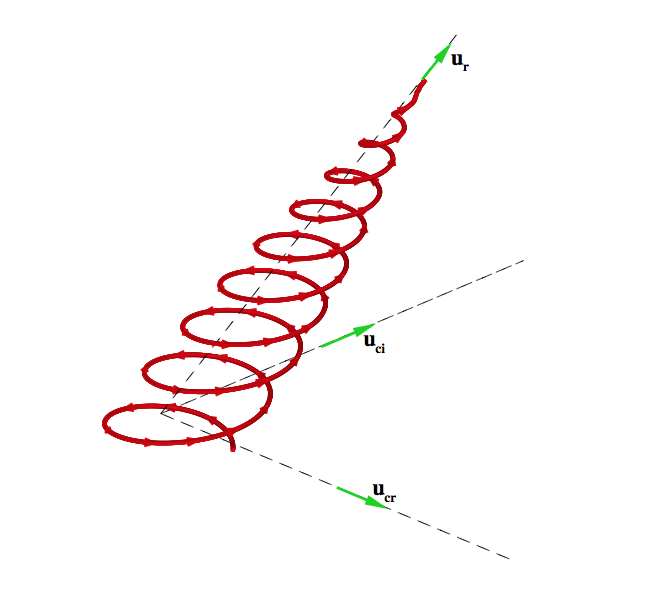
\includegraphics[clip=true, trim= 0.0cm 0.0cm 0.0cm 0.0cm,width=0.99\linewidth]{./figures/vorcord} 
\caption{Illustration of the vortex system \cite{mohamed2012eddy}.}
\end{figure}
%%%%%%%%%%%%%%%%%%%%%%%%%%%%%%%%%%%
The concept of the eddy-preserving limiter is to prevent the slope limiter to be activated (or to use a less dissipative limiter) during the reconstruction of the velocity component along the tangential direction of a vortex. To identify vortical flow regions, the enhanced swirling strength criterion of Chakraborty et al. \cite{chakraborty2005relationships} is employed, whereby in a vortical region, the velocity gradient tensor $\pmb\bigtriangledown\mathbf{v}$ possesses a conjugate pair of complex eigenvalues,
\begin{align} 
\sigma ( \pmb \bigtriangledown \mathbf{v})=  \left \{\lambda_{r}, \lambda_{cr}+i\lambda_{ci}, \lambda_{cr}-i\lambda_{ci} \right \}, \left |\lambda_{ci}\right | > \epsilon, \end{align}
where $\epsilon$ is a small positive real number. A local measure for the compactness of the vortical motion is added to further limit the vortical regions to areas where the following condition is satisfied,
\begin{align} 
-\zeta \leq \frac{\lambda_{cr}}{\lambda_{ci}}\leq \delta, \label{eq:1}
\end{align}
where $\zeta$ and $\delta$ are positive thresholds for verifying the compactness of the vortex. The velocity gradient tensor can be decomposed into the following form,
\begin{align} 
\pmb\bigtriangledown\mathbf{v}=\begin{bmatrix}
\hat{\mathbf{u}}_{r} & \hat{\mathbf{u}}_{cr} & \hat{\mathbf{u}}_{ci} 
\end{bmatrix}
\begin{bmatrix}
 \lambda_{r}&0&0 \\ 
 0&\lambda_{cr}&\lambda_{ci}\frac{\left |\mathbf{u}_{cr}\right |}{\left |\mathbf{u}_{ci}\right |}\\ 
 0&-\lambda_{ci}\frac{\left |\mathbf{u}_{ci}\right |}{\left |\mathbf{u}_{cr}\right |}&\lambda_{cr} 
\end{bmatrix}
\begin{bmatrix}
\hat{\mathbf{u}}_{r} & \hat{\mathbf{u}}_{cr} & \hat{\mathbf{u}}_{ci} 
\end{bmatrix}^{-1},
\end{align}
where $\hat{\mathbf{u}}_{r}$, $\hat{\mathbf{u}}_{cr}$, and $\hat{\mathbf{u}}_{ci}$ are normalized eigenvectors of the velocity gradient tensor.
%%%%%%%%%%%%%%%%%%%%%%%%%%%%%%%%%%%
The mapping and transformation matrix from the original Cartesian system $\mathbf{S}_{0}$ to the local vortex system $\mathbf{S}_{\omega}$ spanned by $\hat{\mathbf{u}}_{r}$, $\hat{\mathbf{u}}_{cr}$, and $\hat{\mathbf{u}}_{ci}$, are given by,
\begin{align} 
\begin{bmatrix}
\hat{\mathbf{M}}
\end{bmatrix}:\mathbf{S}_{0} \mapsto \mathbf{S}_{\omega}\; \; \; \; \; \begin{bmatrix}
\hat{\mathbf{M}}
\end{bmatrix}=\begin{bmatrix}
\hat{\mathbf{u}}_{r} & \hat{\mathbf{u}}_{cr} & \hat{\mathbf{u}}_{ci} 
\end{bmatrix}^{-1}.
\end{align}
The algorithm for the eddy-preserving limiting procedure is described below:
\renewcommand{\labelenumi}{\arabic{enumi}.}
\begin{enumerate}[nolistsep]

\item Calculate eigenvalues of the velocity gradient tensor $\pmb\bigtriangledown\mathbf{v}$. If the velocity gradient tensor has only real eigenvalues, then exit and employ the conventional van Albada limiter.

\item Verify the compactness of the vortical motion using Eqn.~\ref{eq:1}. If the flow lacks vortical compactness, then exit and employ the conventional van Albada limiter.

\item Calculate eigenvectors of the velocity gradient tensor $\pmb\bigtriangledown\mathbf{v}$, and define the transformation matrix $\begin{bmatrix}
\hat{\mathbf{M}}
\end{bmatrix}$. 

\item Transform velocity components into the vortex system $\mathbf{S}_{\omega}$.

\item In the axial direction, reconstruct variables using the conventional van Albada limiter with $\kappa=\frac{1}{3}$.

\item In the swirl plane, reconstruct variables using a higher $\kappa$ which leads to less artificial dissipation and inactivate the van Albada limiter by setting $\Phi_{i} = \Phi_{i+1} = 1$. 

\item Transform interpolated velocity components back to the original system $\mathbf{S}_{0}$ and evaluate the fluxes.
% These variables are ready for computing fluxes.
\end{enumerate}

%\begin{align} % requires amsmath; align* for no eq. number
%\mathbf{V}_{i+\frac{1}{2}}^{L}=\mathbf{V}_{i}+\frac{\Phi_{i} }{4}[(1-\kappa )(\mathbf{V}_{i}-\mathbf{V}_{i-1})+(1+\kappa)(\mathbf{V}_{i+1}-\mathbf{V}_{i})],
%\end{align}
%\begin{align} % requires amsmath; align* for no eq. number
%\mathbf{V}_{i+\frac{1}{2}}^{R}=\mathbf{V}_{i+1}-\frac{\Phi_{i+1} }{4}[(1-\kappa )(\mathbf{V}_{i+1}-\mathbf{V}_{i})+(1+\kappa)(\mathbf{V}_{i+2}-\mathbf{V}_{i+1})],
%\end{align}




\subsection{Extended Eddy-Preserving Limiter Scheme}
To extend the eddy-preserving limiter, the van Albada limiter for the interpolation of pressure is switched off at smooth extrema. By setting $\Phi_{i}=\Phi_{i+1}=1$, the interpolation for pressure at smooth extrema is given by,
\begin{align} 
p_{i+\frac{1}{2}}^{L}&=p_{i}+\frac{1}{4}[(1-\kappa )\Delta _{i-\frac{1}{2}}^{u} p+(1+\kappa)\Delta _{i+\frac{1}{2}}^{c} p], \\
p_{i+\frac{1}{2}}^{R}&=p_{i+1}-\frac{1}{4}[(1-\kappa )\Delta _{i+\frac{3}{2}}^{u} p+(1+\kappa)\Delta _{i+\frac{1}{2}}^{c} p].
\end{align}
The smooth extrema is detected based on a criterion proposed by Huynh \cite{huynh1995accurate}. If the solution is smooth at the extremum, then the second-difference in neighbouring cells are comparable. Define the second-difference of $p$ as,
\begin{align} 
\Delta _{i}^{2} p = p_{i-1}-2p_{i}+p_{i+1}.
\end{align}
If the following conditions are satisfied,
\begin{align} 
\frac{4}{5}\le \frac{{\Delta} _{i-1}^{2} p}{{\Delta} _{i}^{2} p}\le \frac{5}{4}, \\
\frac{4}{5}\le \frac{{\Delta} _{i+1}^{2} p}{{\Delta} _{i}^{2} p}\le \frac{5}{4}, 
\end{align}
then the extremum is considered to be smooth, and the limiting is unnecessary. As remarked by Huynh \cite{huynh1995accurate}, the factors $\frac{4}{5}$ and $\frac{5}{4}$ can be relaxed to $\frac{2}{3}$ and $\frac{3}{2}$ for the case of linear convection.
%%%%%%%%%%%%%%%%%%%%%%%%%%%%%%%%%%%%%%%%%%%%%%%%%%%%%%%%%%%%%%%%%%%%%%%
\section{Numerical Results} 

\subsection{Three Dimensional Inviscid Vortex Advection}
An inviscid vortex advection case is designed to demonstrate the effects of the eddy-preserving limiter schemes. The direction of advection is perpendicular to the vortex surface, as illustrated in Fig.~\ref{vortex3d}.
The flow field is initialized as an isentropic vortex superimposed by a uniform flow, where $u_{\infty}=0$, $v_{\infty}=0$ and $w_{\infty}=1$. The flow variables are computed by:
\begin{align}
\begin{split} 
\rho&=[1-\frac{(\gamma-1)\beta^{2}}{8\gamma\pi^{2}}e^{1-r^{2}}]^{1/(\gamma-1)}, \\
u&=u_{\infty}+\delta u=- \frac{\beta y}{2\pi}e^{(1-r^{2})/2}, \\
v&=v_{\infty}+\delta v= \frac{\beta x}{2\pi}e^{(1-r^{2})/2}, \\
w&=w_{\infty}, \\
p&=\rho ^{\gamma},
\end{split}
\label{vor-equ}
\end{align}
where the centre of the vortex is located at $(x,y)=(0,0)$, $r=\sqrt{x^2+y^2}$ represents the distance to the centre of the vortex, and $\beta$ is the vortex strength and is set to a value of 5.
%%%%%%%%%%%%%%%%%%%%%%%%%%%%%%%%%%%
\begin{figure}[t]  
\centering
     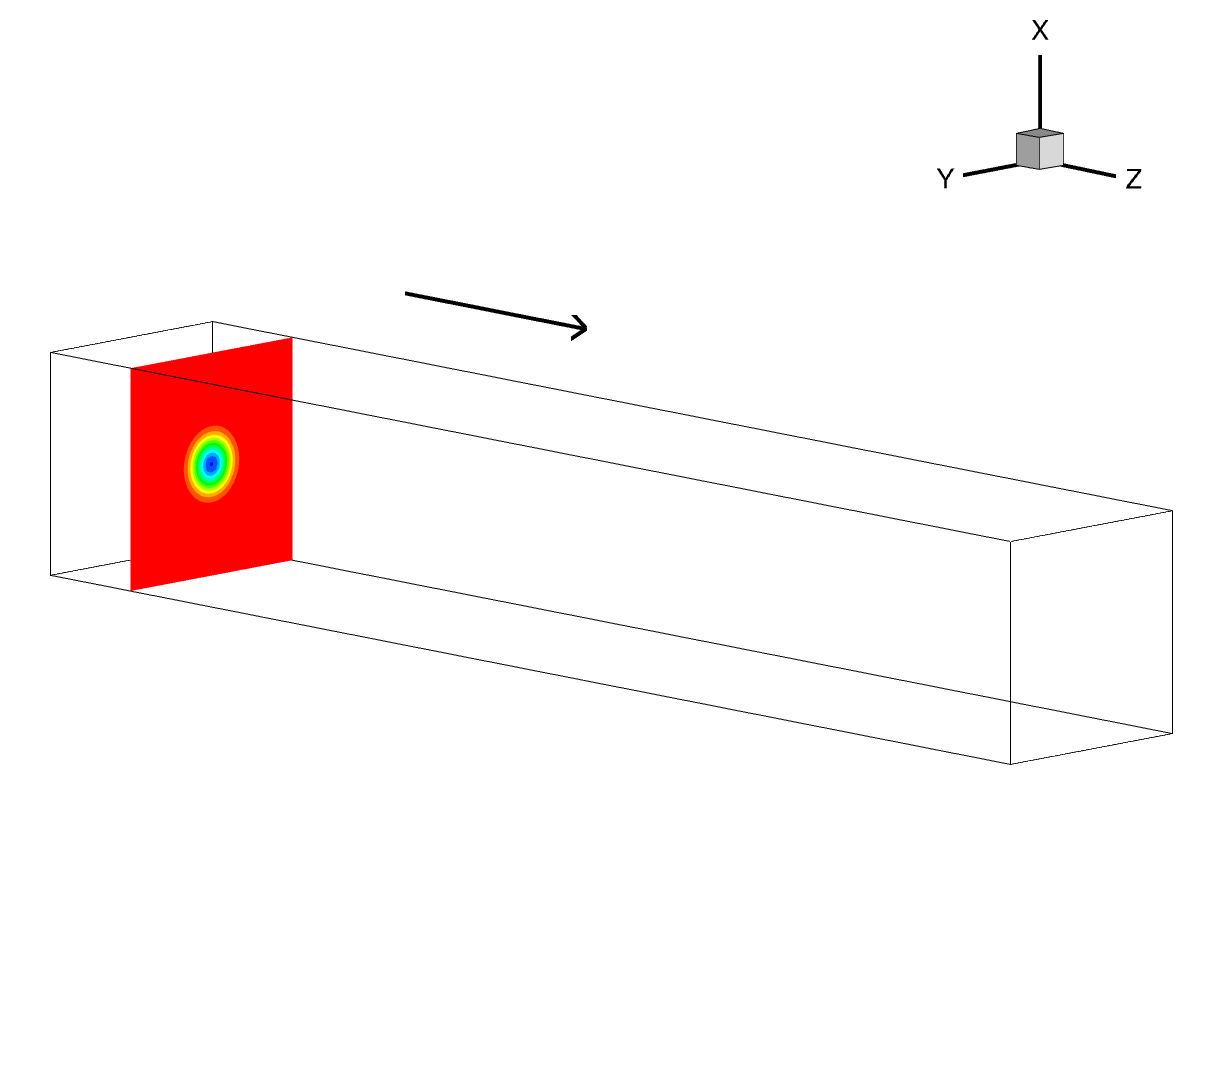
\includegraphics[clip=true, trim= 1.75cm 11.0cm 1.75cm 0.5cm,width=0.99\linewidth]{./figures/vortex3d/vortex3d}                  
     \caption{Illustration of the vortex advection.}
     \label{vortex3d}
\end{figure}
%%%%%%%%%%%%%%%%%%%%%%%%%%%%%%%%%%%
The geometry of the computational domain is a rectangular box, where $-5\le x \le5$, $-5\le y \le 5$, and $0\le z \le 12$. We demonstrate the ability of the schemes to preserve the vortex through a grid refinement study, where the coarse grid has dimensions $\Delta x=\Delta y=\Delta z=0.5$, the medium grid with $\Delta x=\Delta y=\Delta z=0.25$, and the fine grid with $\Delta x=\Delta y=\Delta z=0.125$. The time step is set to be $\Delta t=0.04$ and the final time is $t=10$. The test cases are simulated with the baseline MUSCL scheme, the original and the extended eddy-preserving limiter schemes. The computed results are denoted by ``MUSCL'', ``EDDY'', and ``EDDY-P'' respectively.
%%%%%%%%%%%%%%%%%%%%%%%%%%%%%%%%%%%%%%%%%%%%%%%%%%%%%%%%%%%%%%%%
\begin{figure*}[t]
\centering
     \subfigure[$t=2$ on coarse grid]{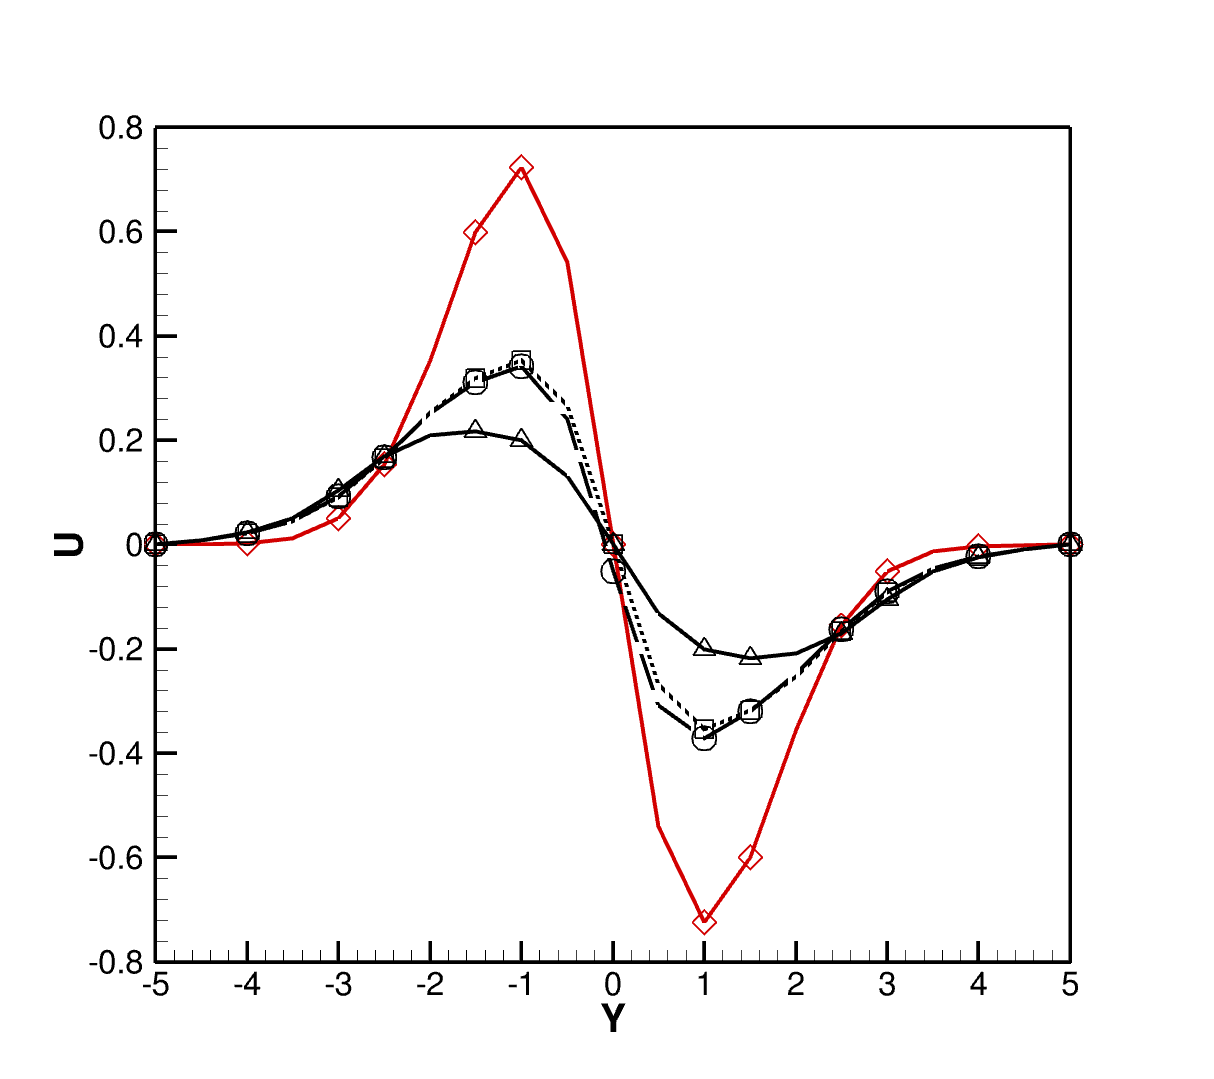
\includegraphics[clip=true, trim= 1.5cm 1.25cm 0.5cm 0.5cm,width=0.325\linewidth]{./figures/vortex3d/04up/04u1}}              
     \subfigure[$t=2$ on medium grid]{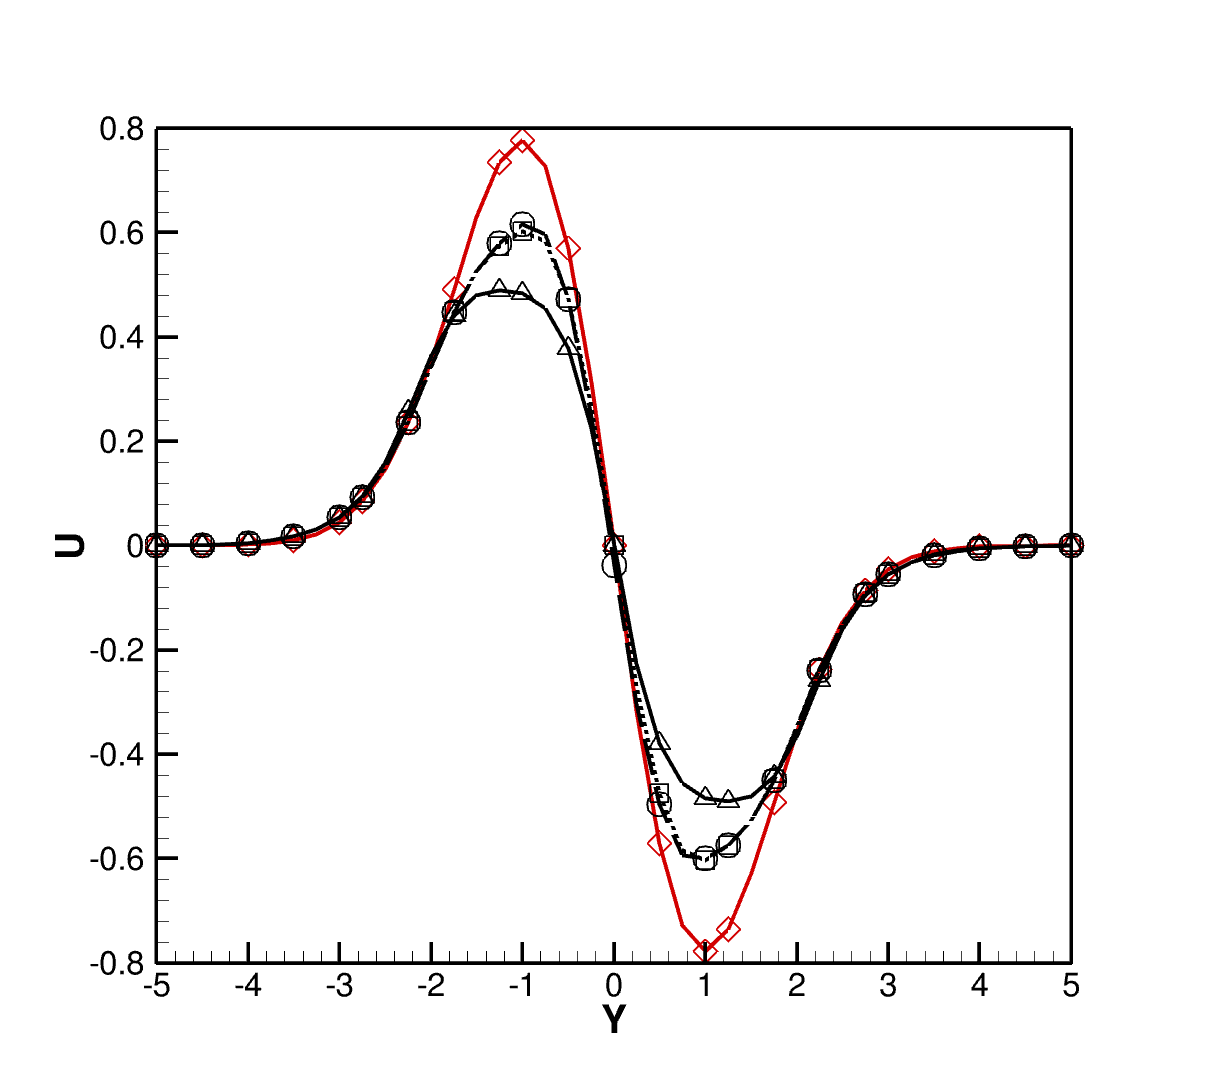
\includegraphics[clip=true, trim= 1.5cm 1.25cm 0.5cm 0.5cm,width=0.325\linewidth]{./figures/vortex3d/03up/03u1}}
     \subfigure[$t=2$ on fine grid]{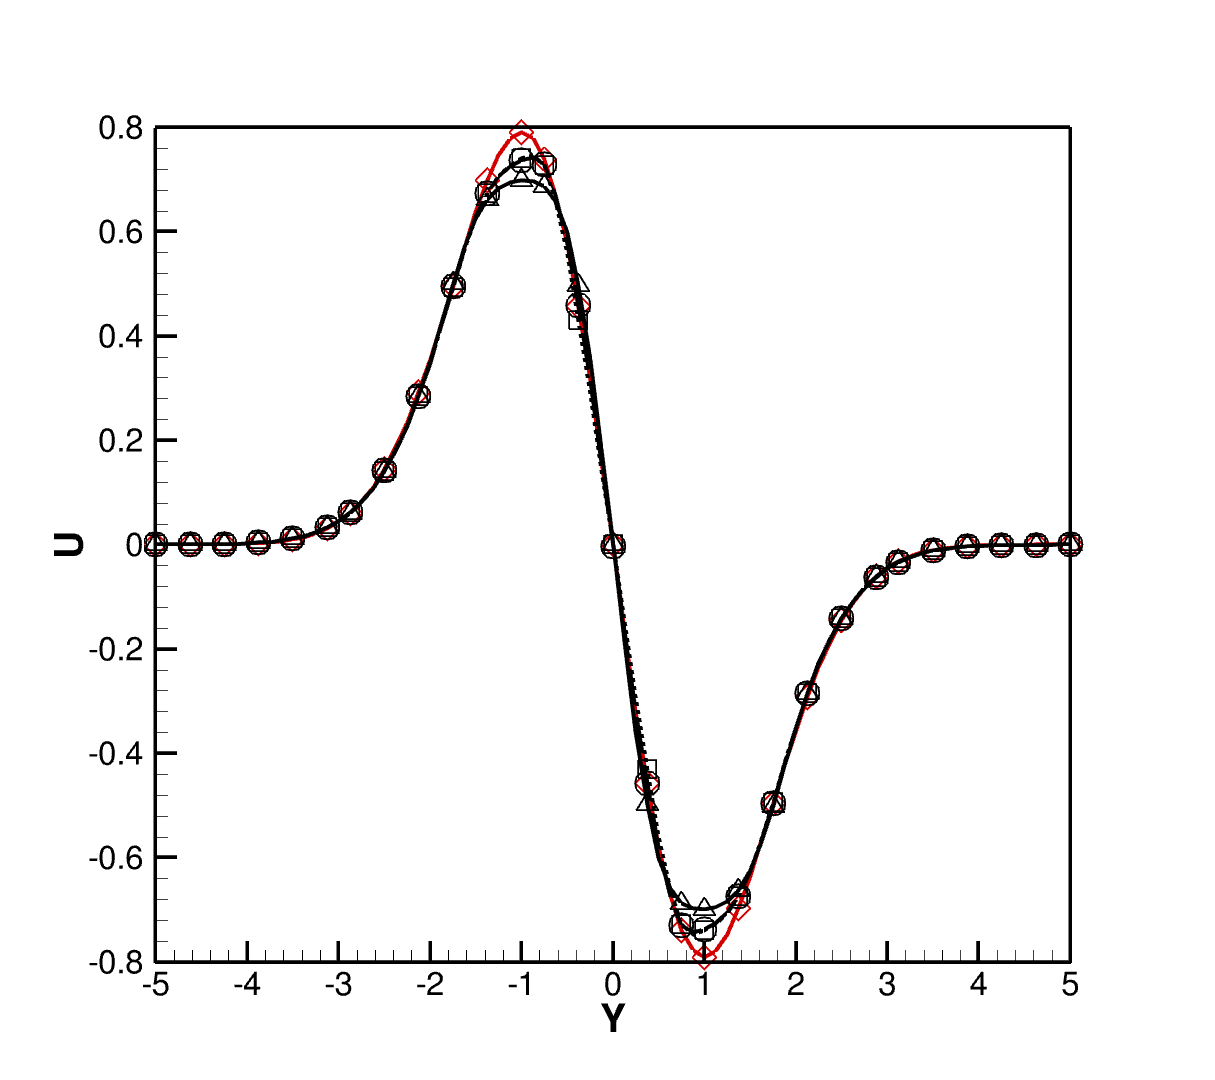
\includegraphics[clip=true, trim= 1.5cm 1.25cm 0.5cm 0.5cm,width=0.325\linewidth]{./figures/vortex3d/05up/05u1}}
     \subfigure[$t=6$ on coarse grid]{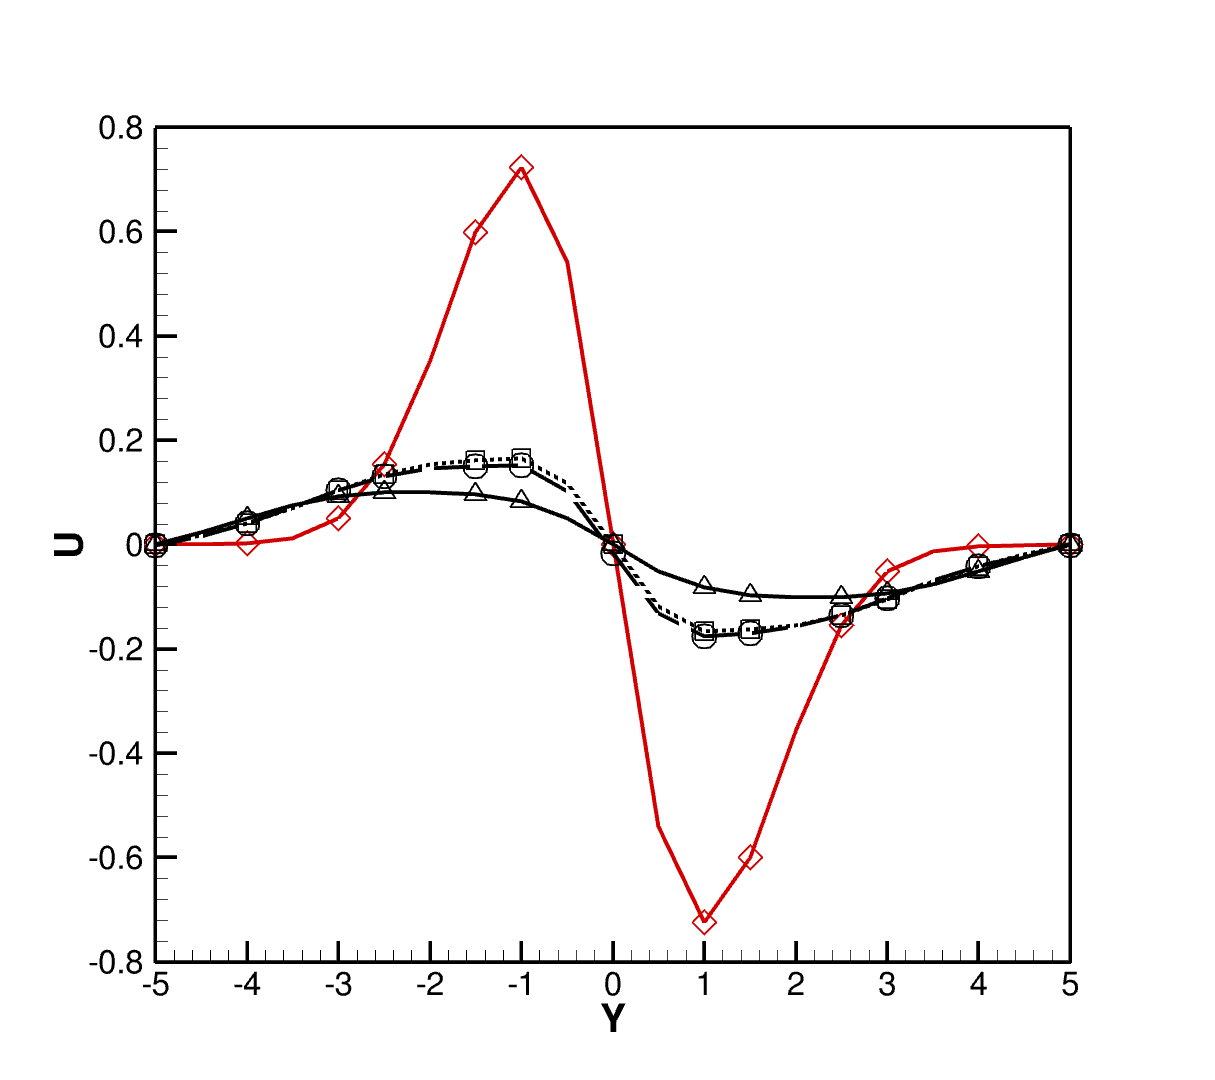
\includegraphics[clip=true, trim= 1.5cm 1.25cm 0.5cm 0.5cm,width=0.325\linewidth]{./figures/vortex3d/04up/04u3}}              
     \subfigure[$t=6$ on medium grid]{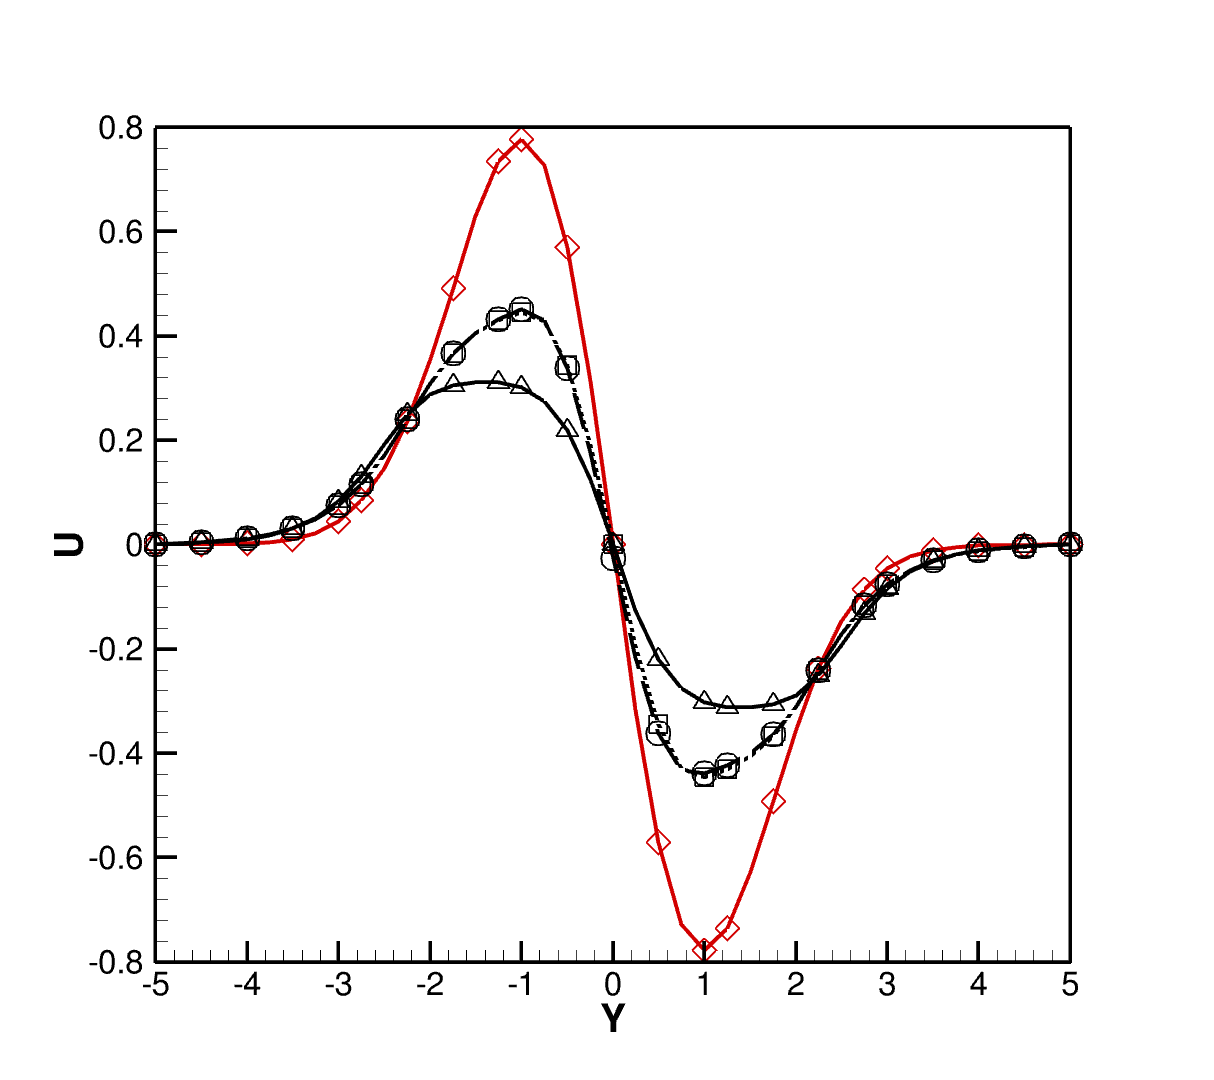
\includegraphics[clip=true, trim= 1.5cm 1.25cm 0.5cm 0.5cm,width=0.325\linewidth]{./figures/vortex3d/03up/03u3}}
     \subfigure[$t=6$ on fine grid]{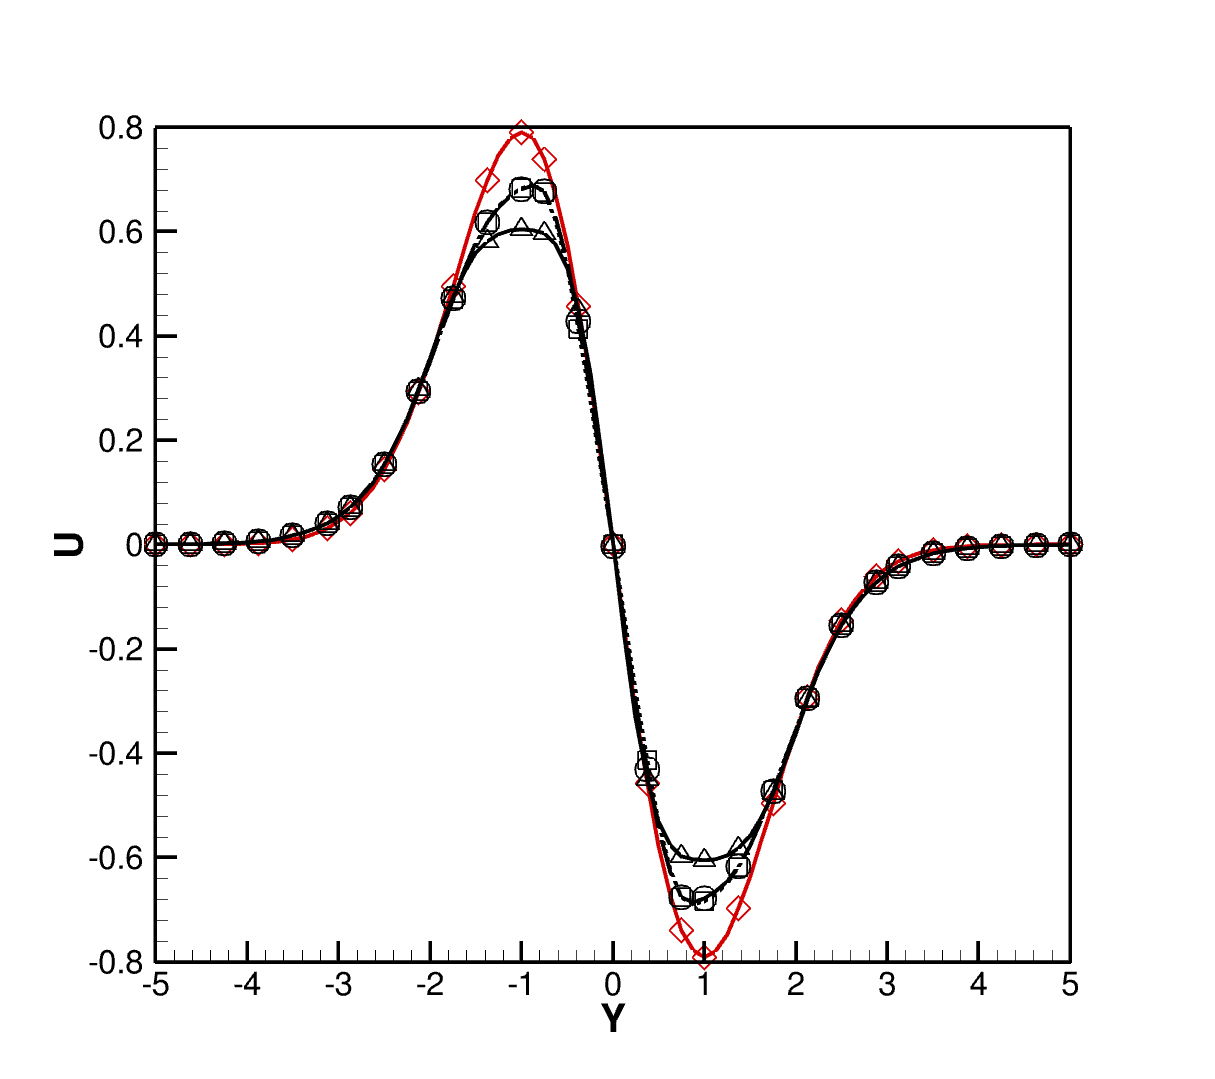
\includegraphics[clip=true, trim= 1.5cm 1.25cm 0.5cm 0.5cm,width=0.325\linewidth]{./figures/vortex3d/05up/05u3}}
     \subfigure[$t=10$ on coarse grid]{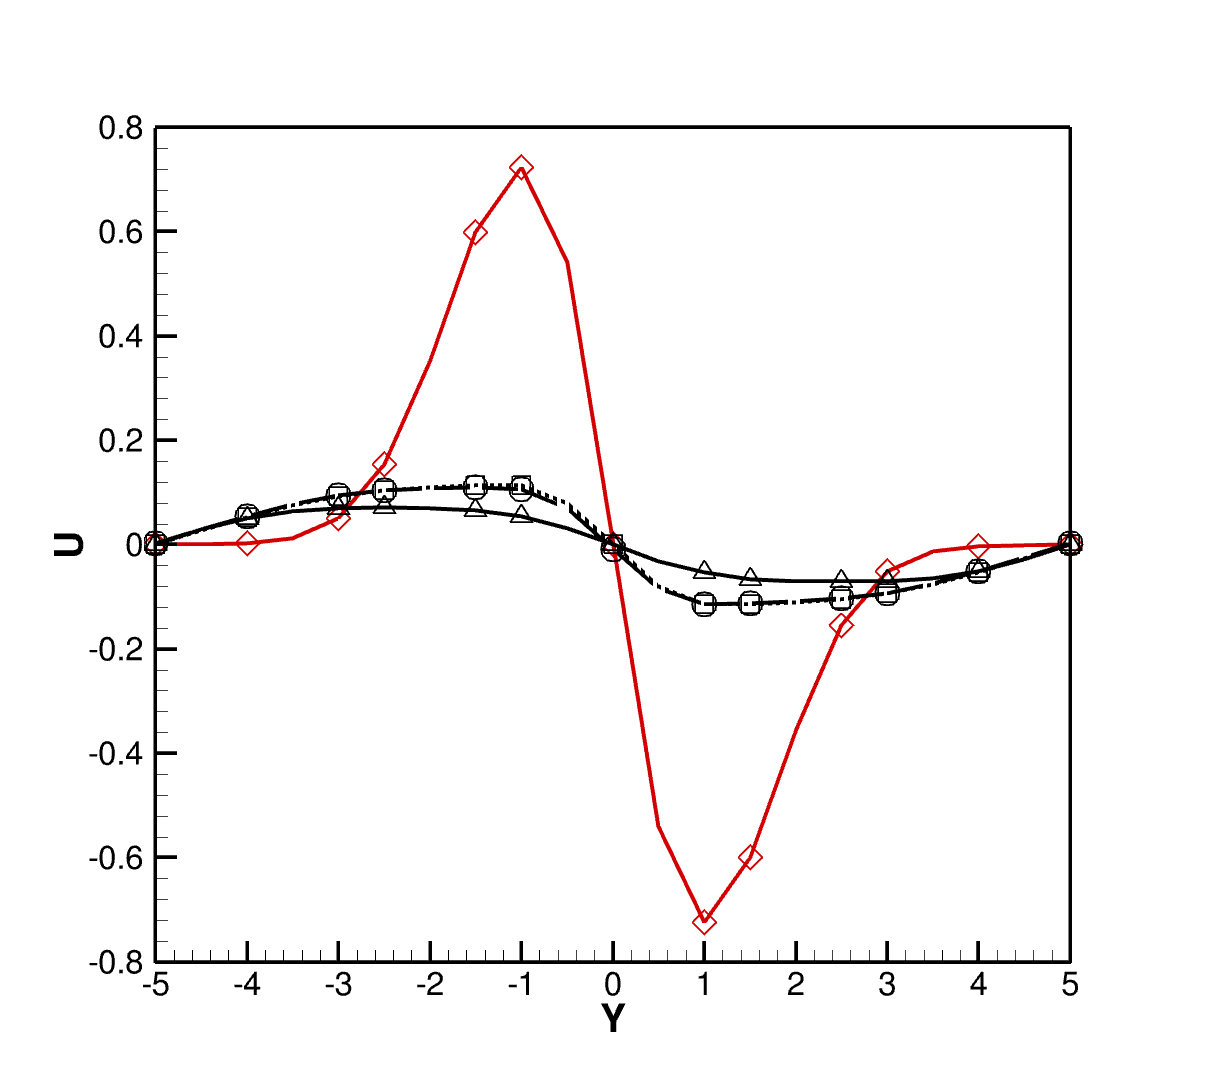
\includegraphics[clip=true, trim= 1.5cm 1.25cm 0.5cm 0.5cm,width=0.325\linewidth]{./figures/vortex3d/04up/04u5}}              
     \subfigure[$t=10$ on medium grid]{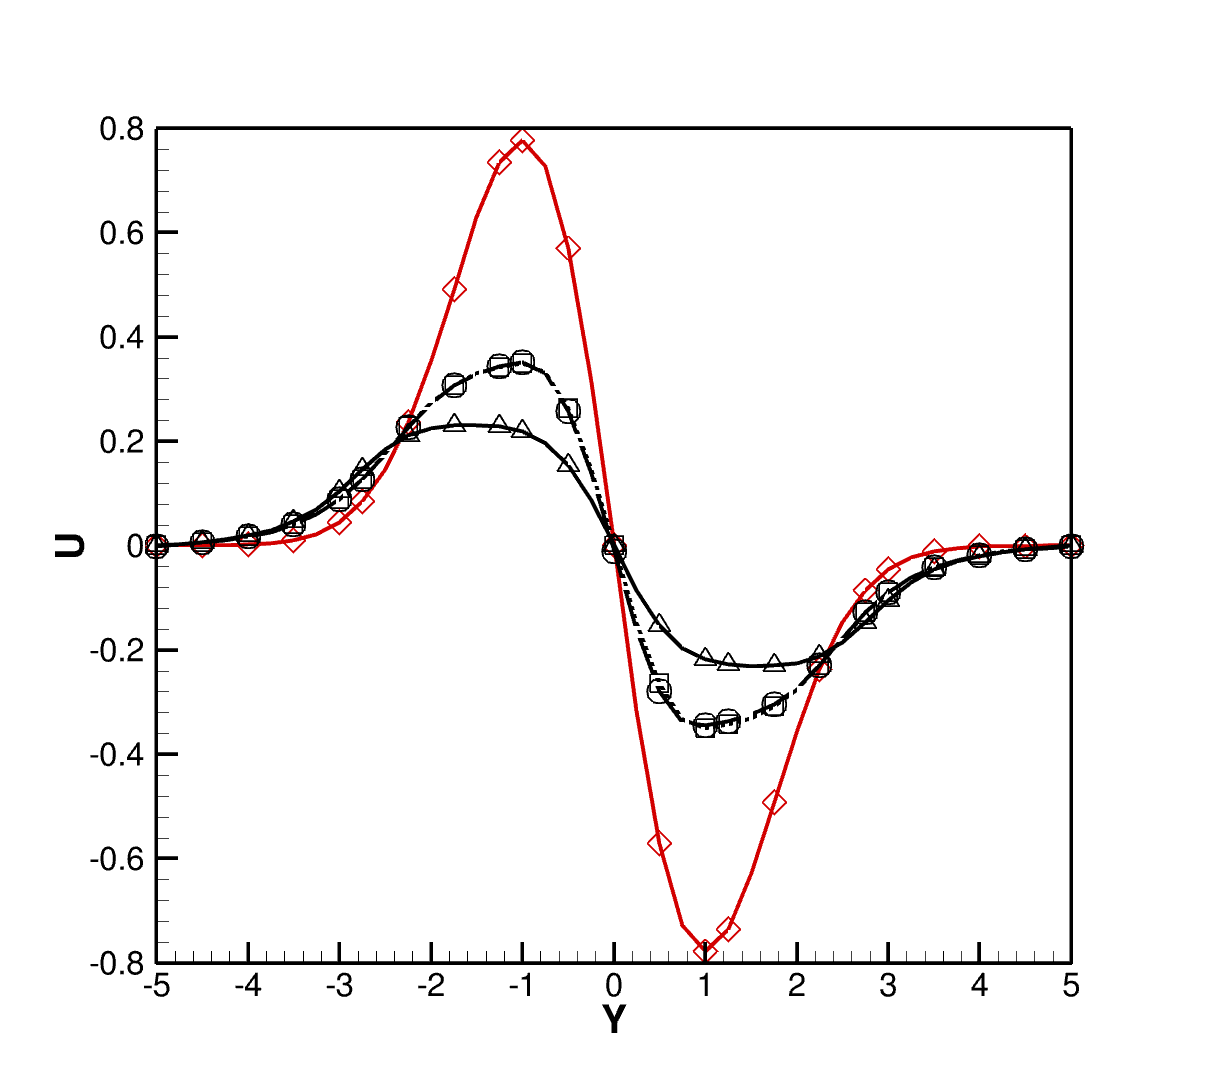
\includegraphics[clip=true, trim= 1.5cm 1.25cm 0.5cm 0.5cm,width=0.325\linewidth]{./figures/vortex3d/03up/03u5}}
     \subfigure[$t=10$ on fine grid]{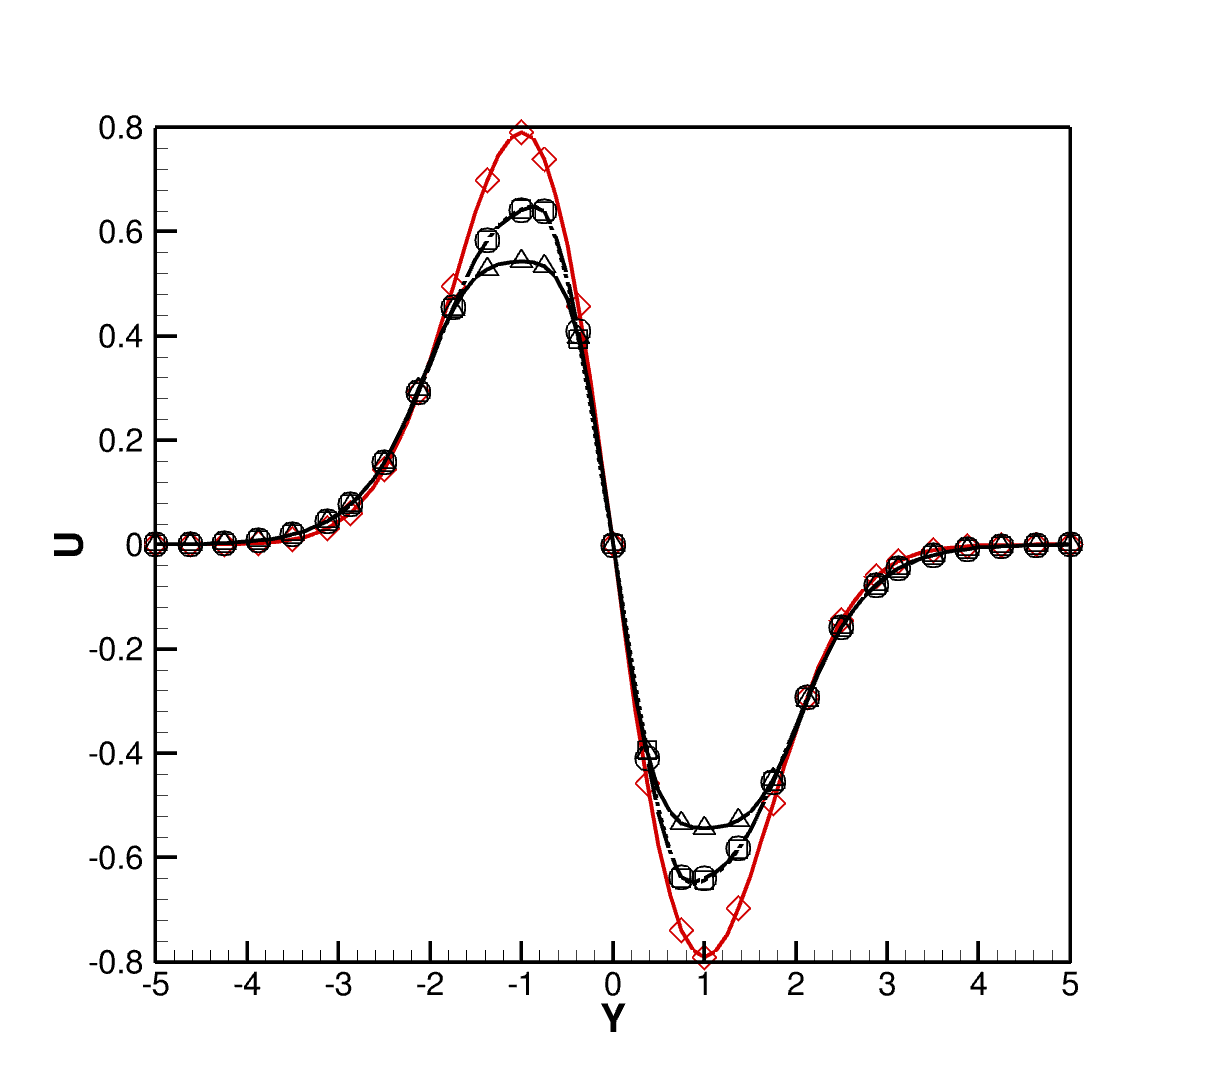
\includegraphics[clip=true, trim= 1.5cm 1.25cm 0.5cm 0.5cm,width=0.325\linewidth]{./figures/vortex3d/05up/05u5}}                   
     \caption{Velocity profiles at $x=0$. (MUSCL: \mline; EDDY: \eline; EDDY-P: \epline; Exact: \exact.)}     
     \label{u135}
\end{figure*}
%%%%%%%%%%%%%%%%%%%%%%%%%%%%%%%%%%%%%%%%%%%%%%%%%%%%%%%%%%%%%%%%
The profiles of the $x$ component of velocity at $x=0$ and several time instances $t=2$, $t=6$, and $t=10$ are shown in Fig.~\ref{u135}. The relative $L^{2}$ norms of the error are plotted in Fig.~\ref{l2} (a). The profiles computed by the EDDY and EDDY-P schemes are similar, and hence the modification for the interpolation of pressure has little impact on the velocity profiles. The predictions of both the EDDY and EDDY-P schemes agree better against the exact solutions when compared to the MUSCL scheme, due to their lower numerical dissipations.
%%%%%%%%%%%%%%%%%%%%%%%%%%%%%%%%%%%%%%%%%%%%%%%%%%%%%%%%%%%%%%%%
\begin{figure*}[t]  
\centering
     \subfigure[$t=2$ on coarse grid]{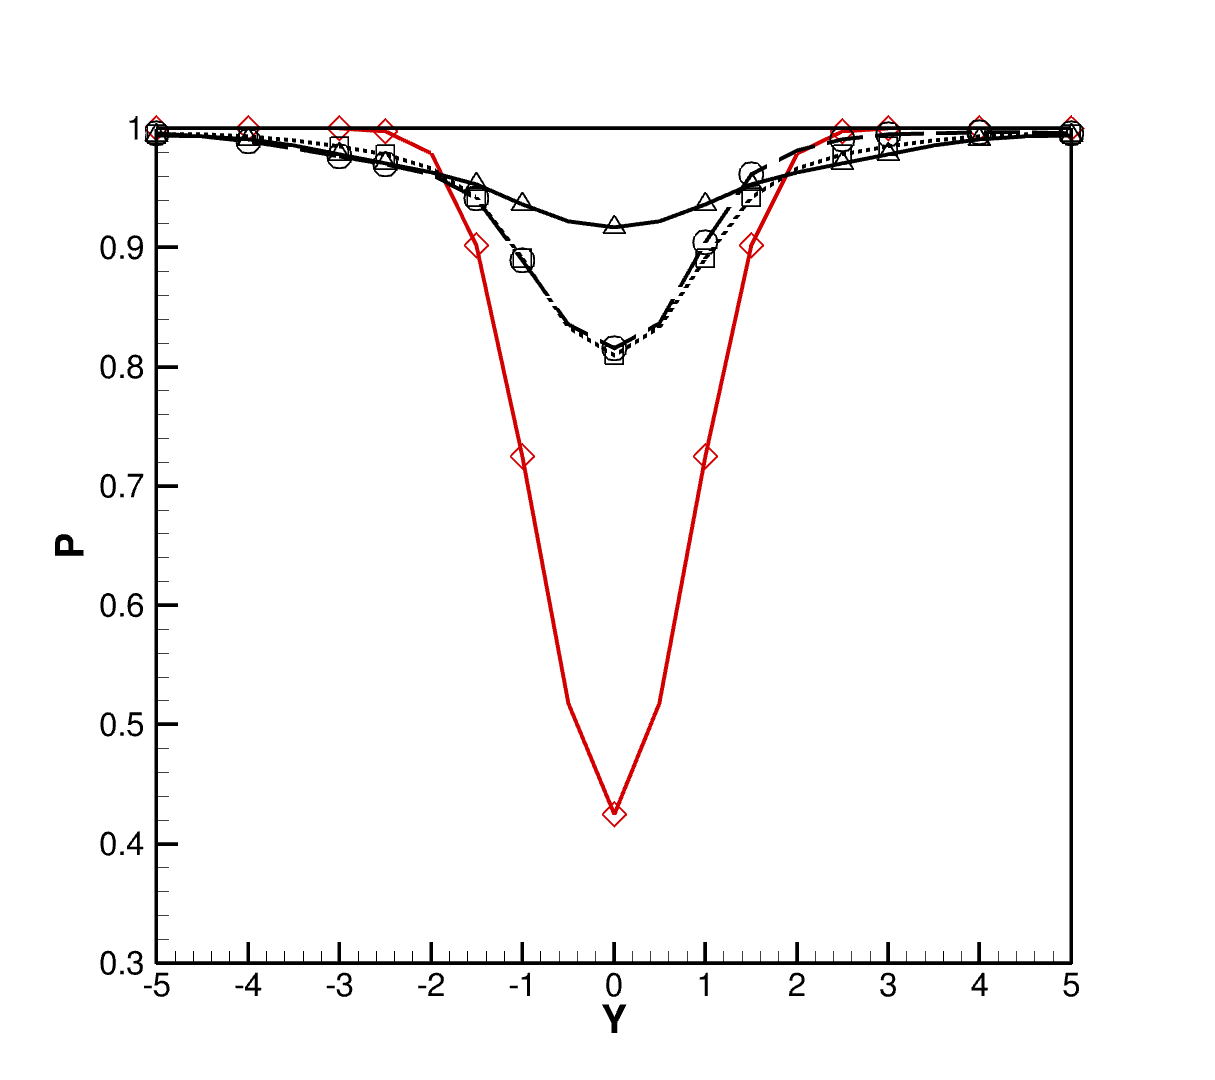
\includegraphics[clip=true, trim= 1.5cm 1.25cm 0.5cm 0.5cm,width=0.325\linewidth]{./figures/vortex3d/04up/04p1}}              
     \subfigure[$t=2$ on medium grid]{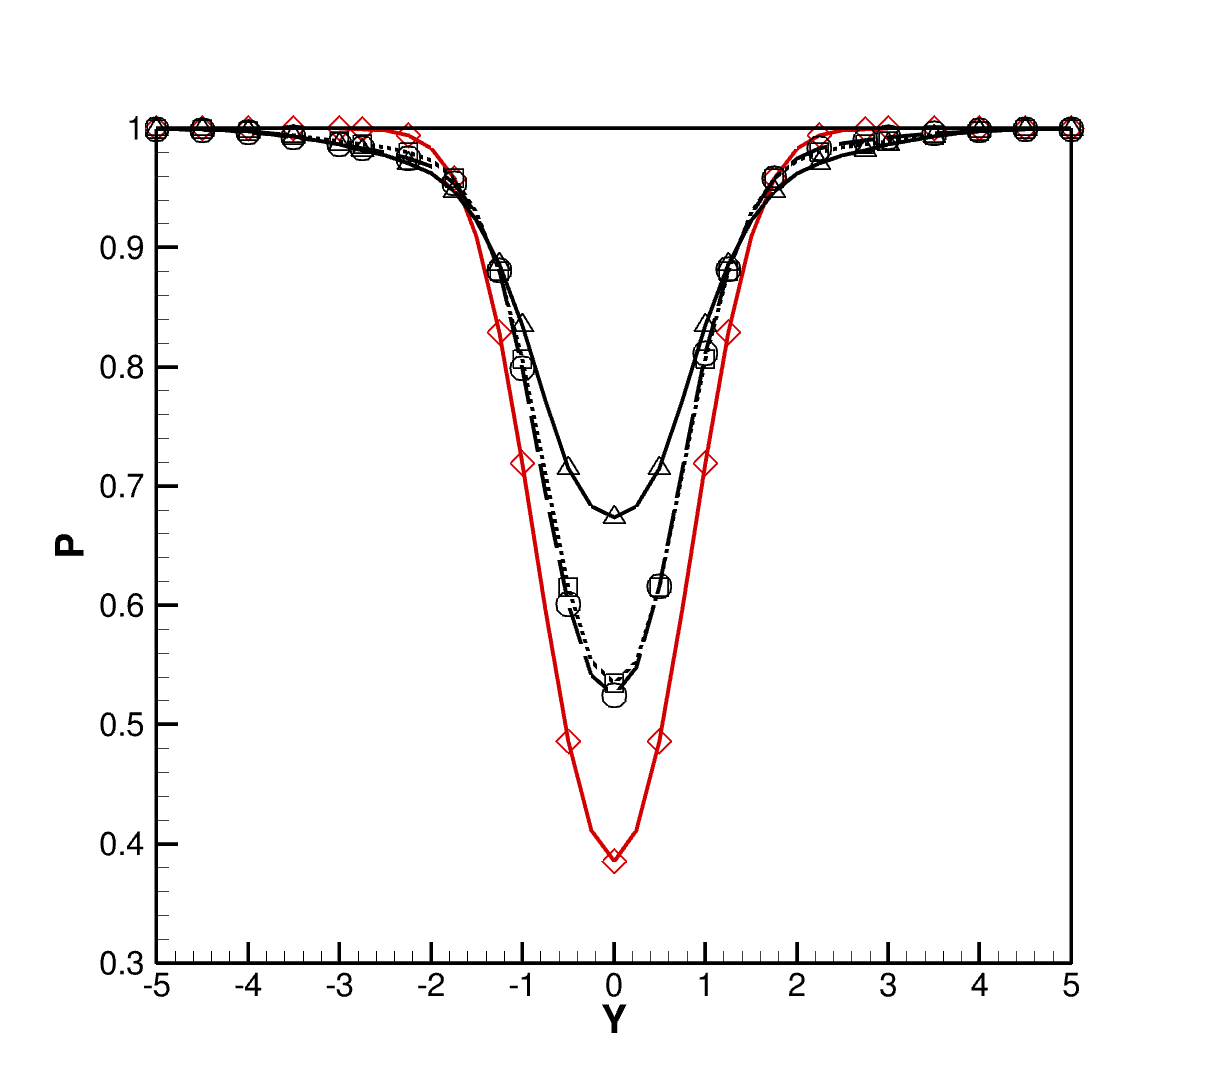
\includegraphics[clip=true, trim= 1.5cm 1.25cm 0.5cm 0.5cm,width=0.325\linewidth]{./figures/vortex3d/03up/03p1}}
     \subfigure[$t=2$ on fine grid]{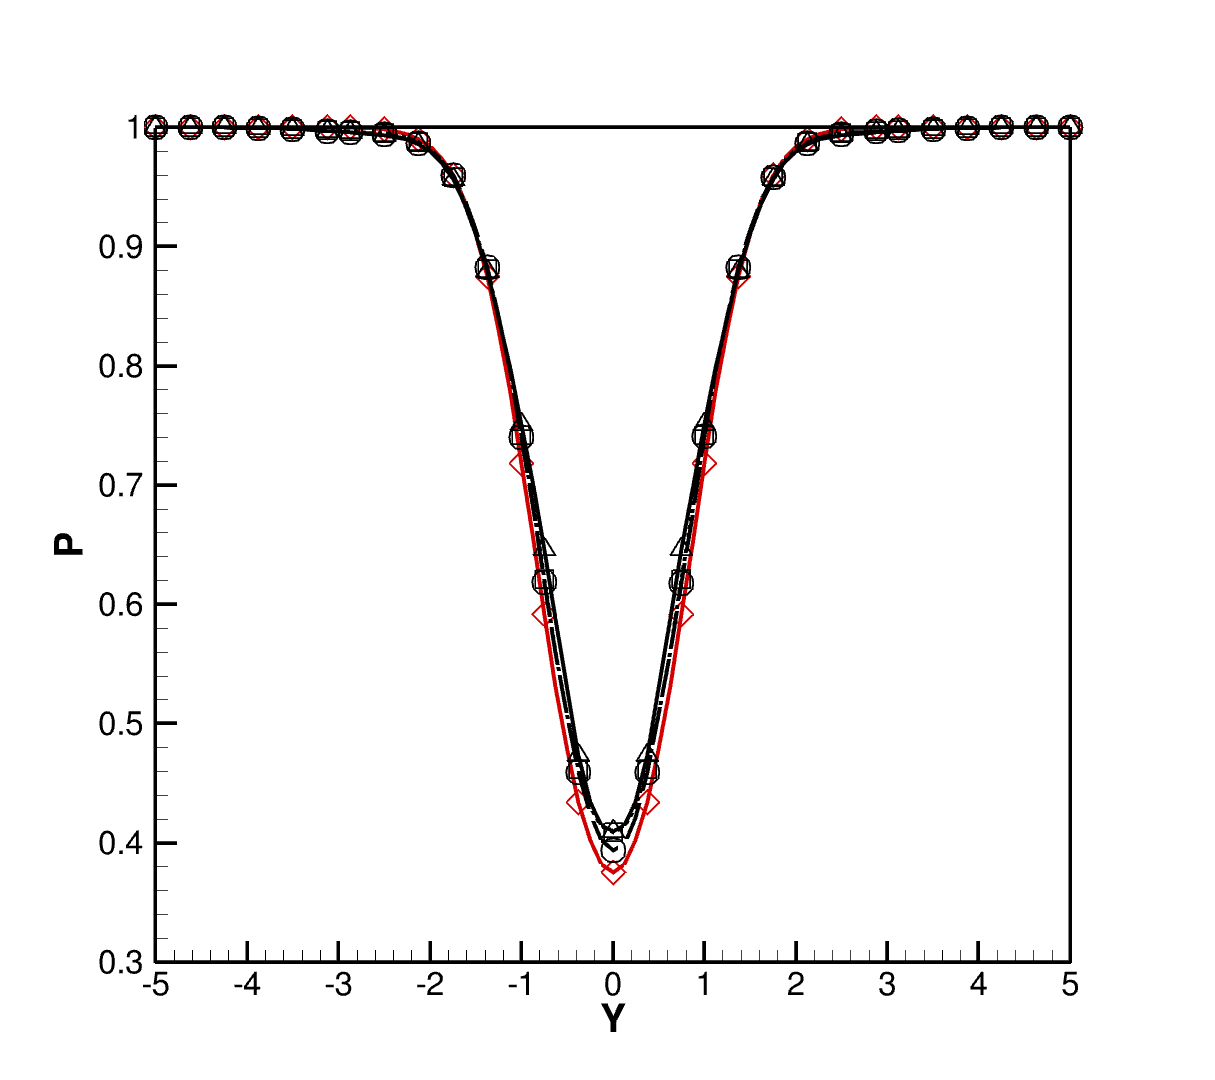
\includegraphics[clip=true, trim= 1.5cm 1.25cm 0.5cm 0.5cm,width=0.325\linewidth]{./figures/vortex3d/05up/05p1}}
     \subfigure[$t=6$ on coarse grid]{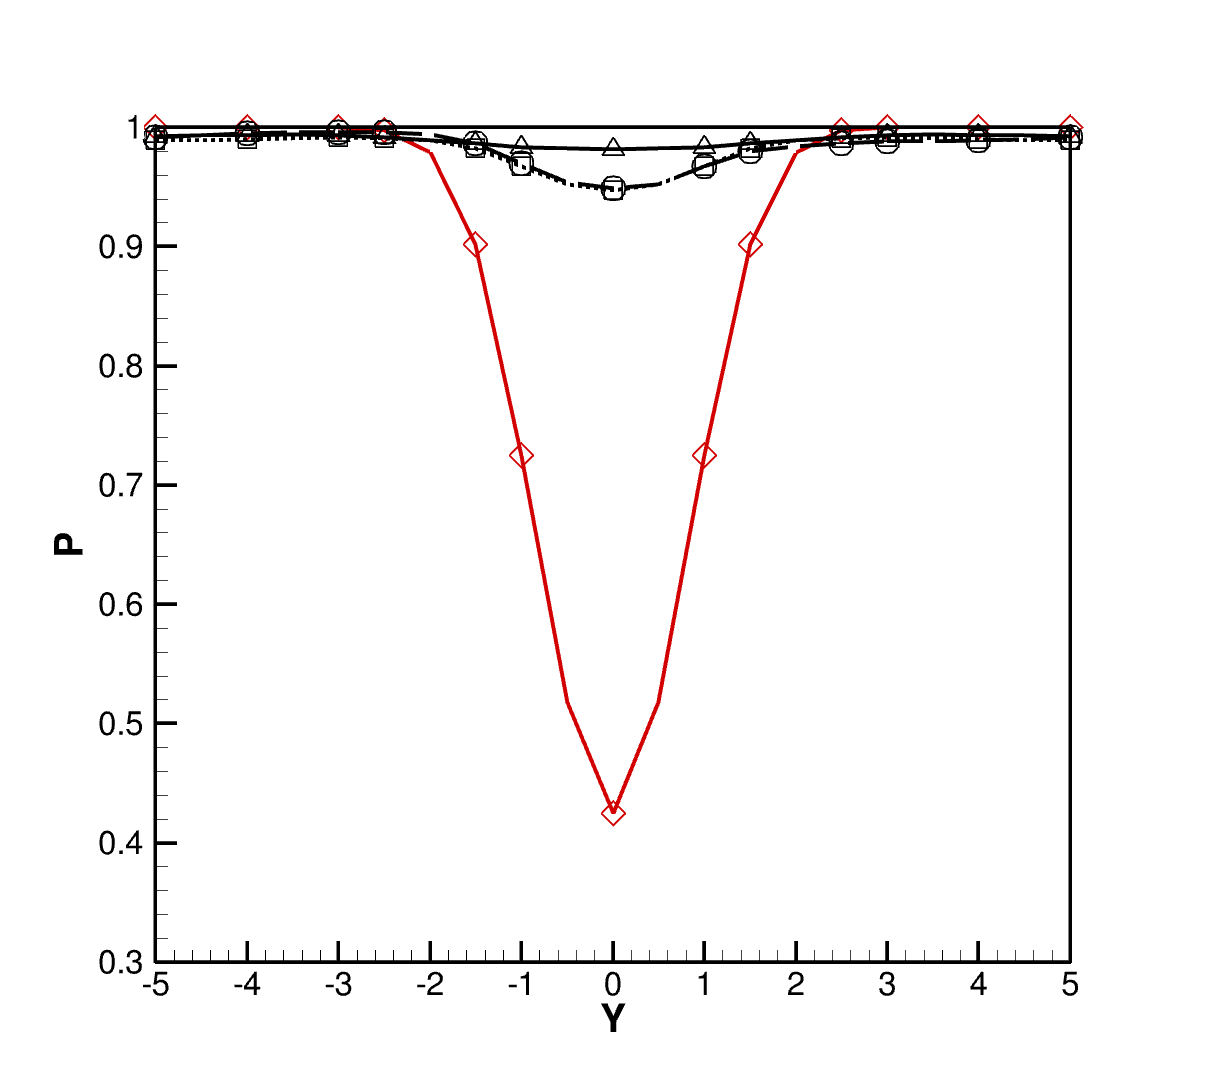
\includegraphics[clip=true, trim= 1.5cm 1.25cm 0.5cm 0.5cm,width=0.325\linewidth]{./figures/vortex3d/04up/04p3}}              
     \subfigure[$t=6$ on medium grid]{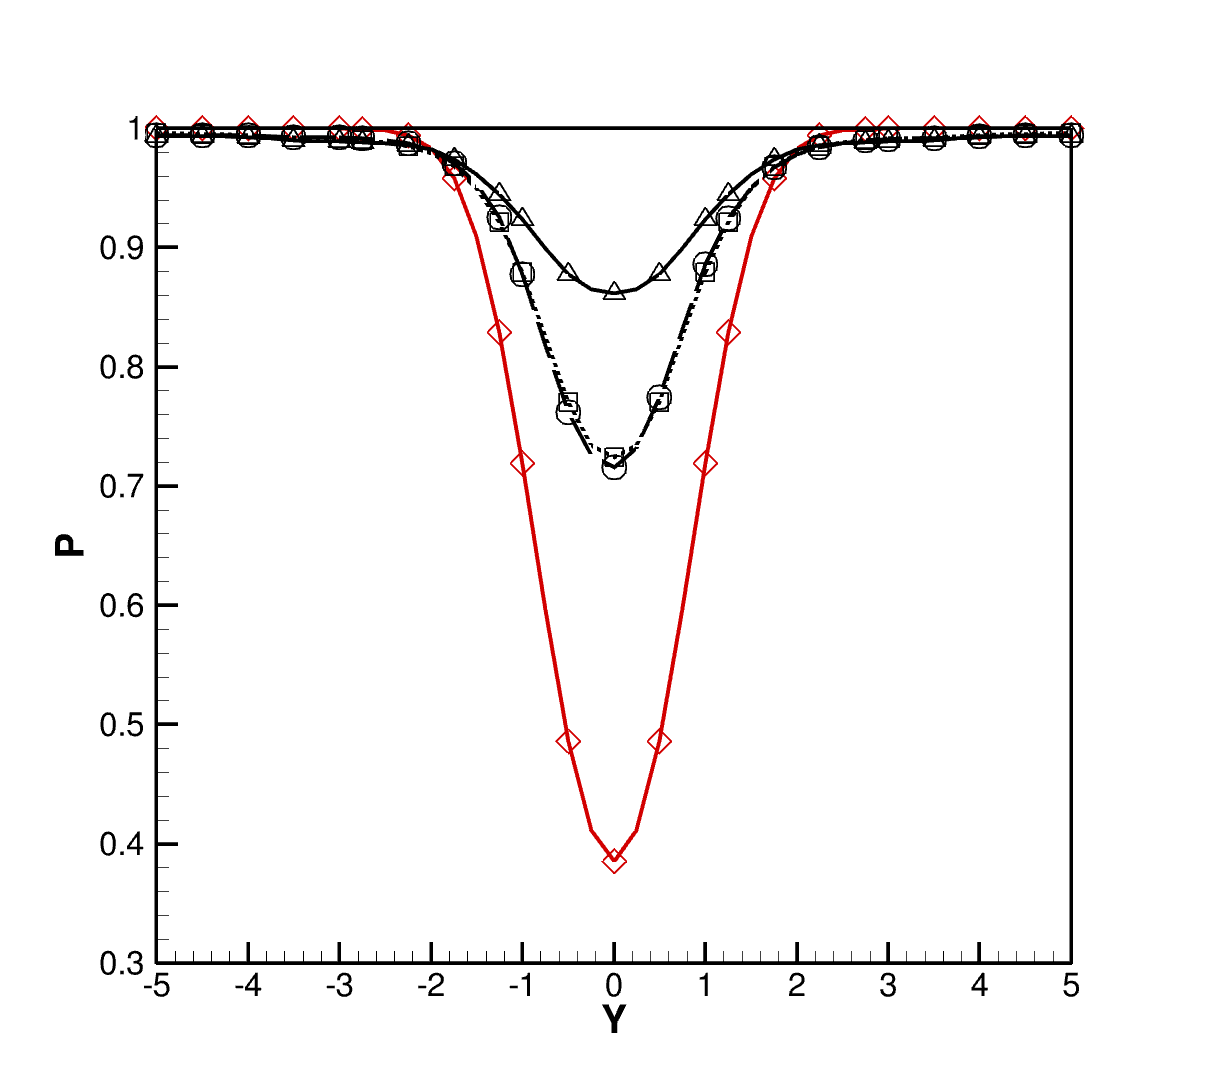
\includegraphics[clip=true, trim= 1.5cm 1.25cm 0.5cm 0.5cm,width=0.325\linewidth]{./figures/vortex3d/03up/03p3}}
     \subfigure[$t=6$ on fine grid]{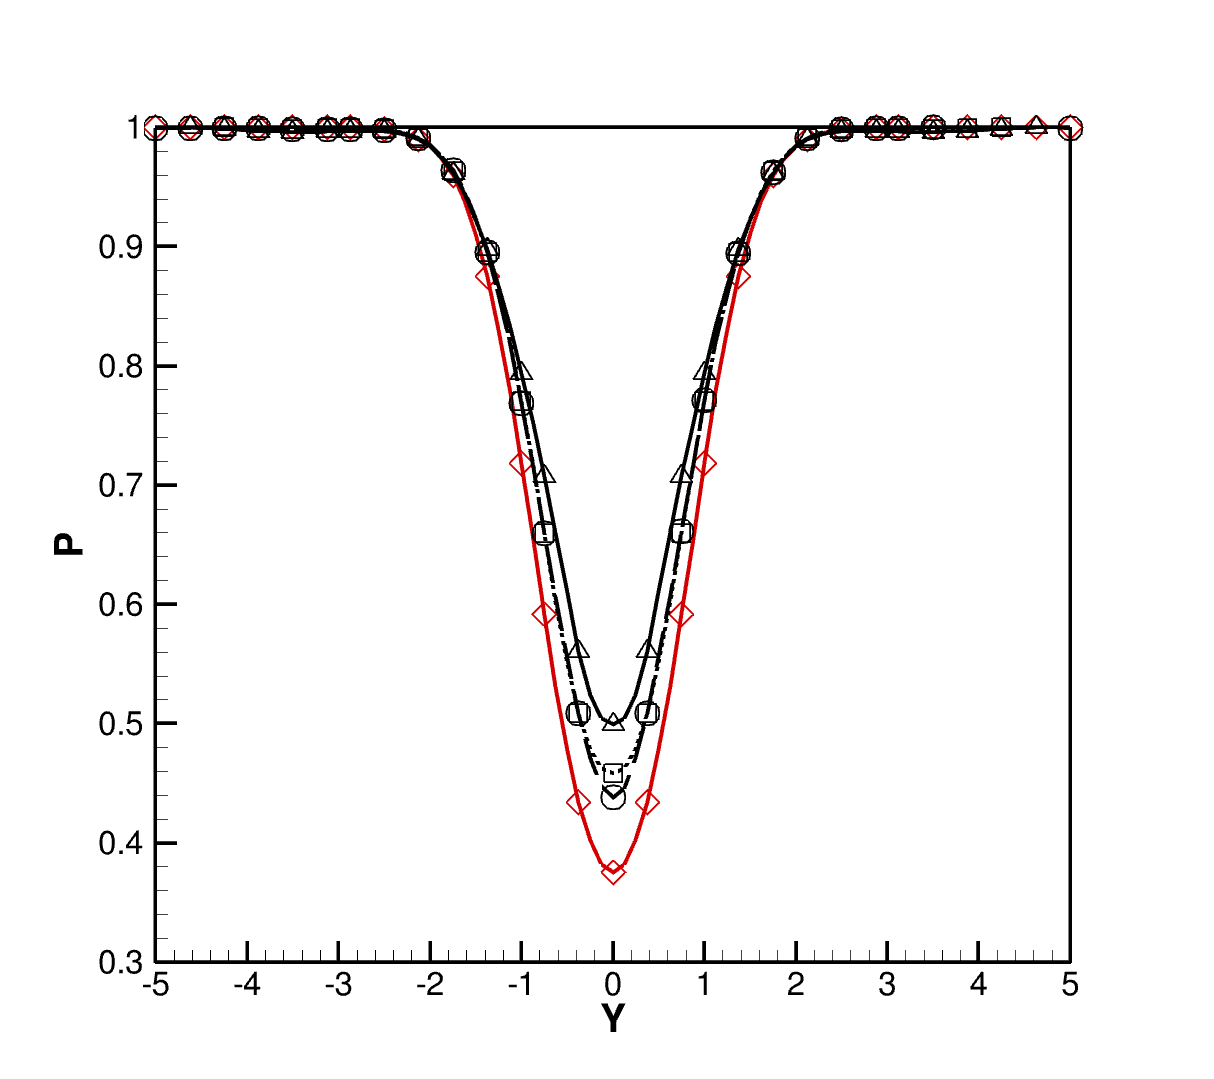
\includegraphics[clip=true, trim= 1.5cm 1.25cm 0.5cm 0.5cm,width=0.325\linewidth]{./figures/vortex3d/05up/05p3}}
     \subfigure[$t=10$ on coarse grid]{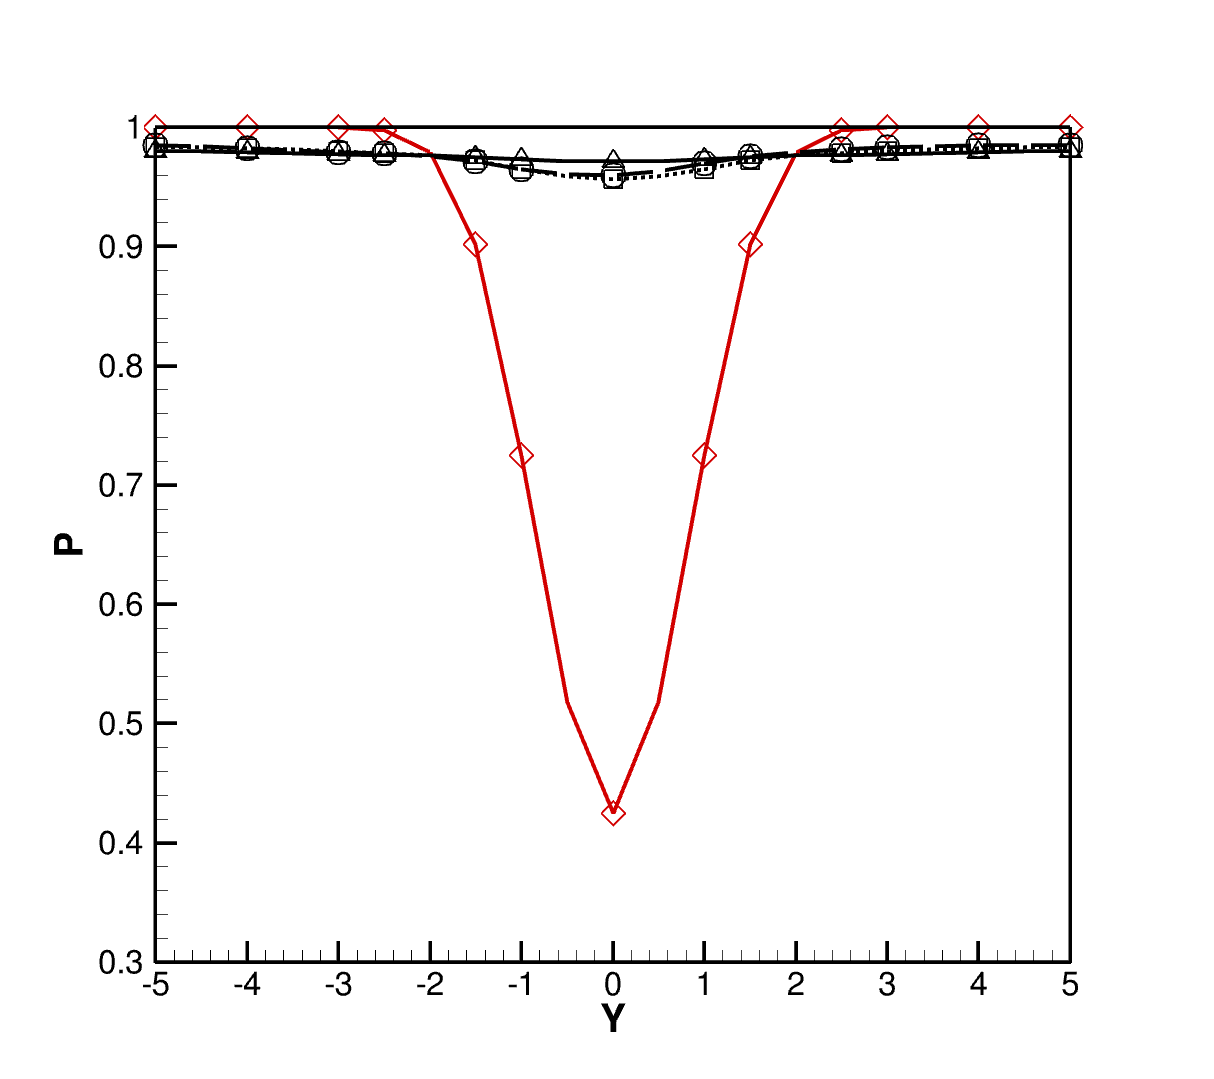
\includegraphics[clip=true, trim= 1.5cm 1.25cm 0.5cm 0.5cm,width=0.325\linewidth]{./figures/vortex3d/04up/04p5}}              
     \subfigure[$t=10$ on medium grid]{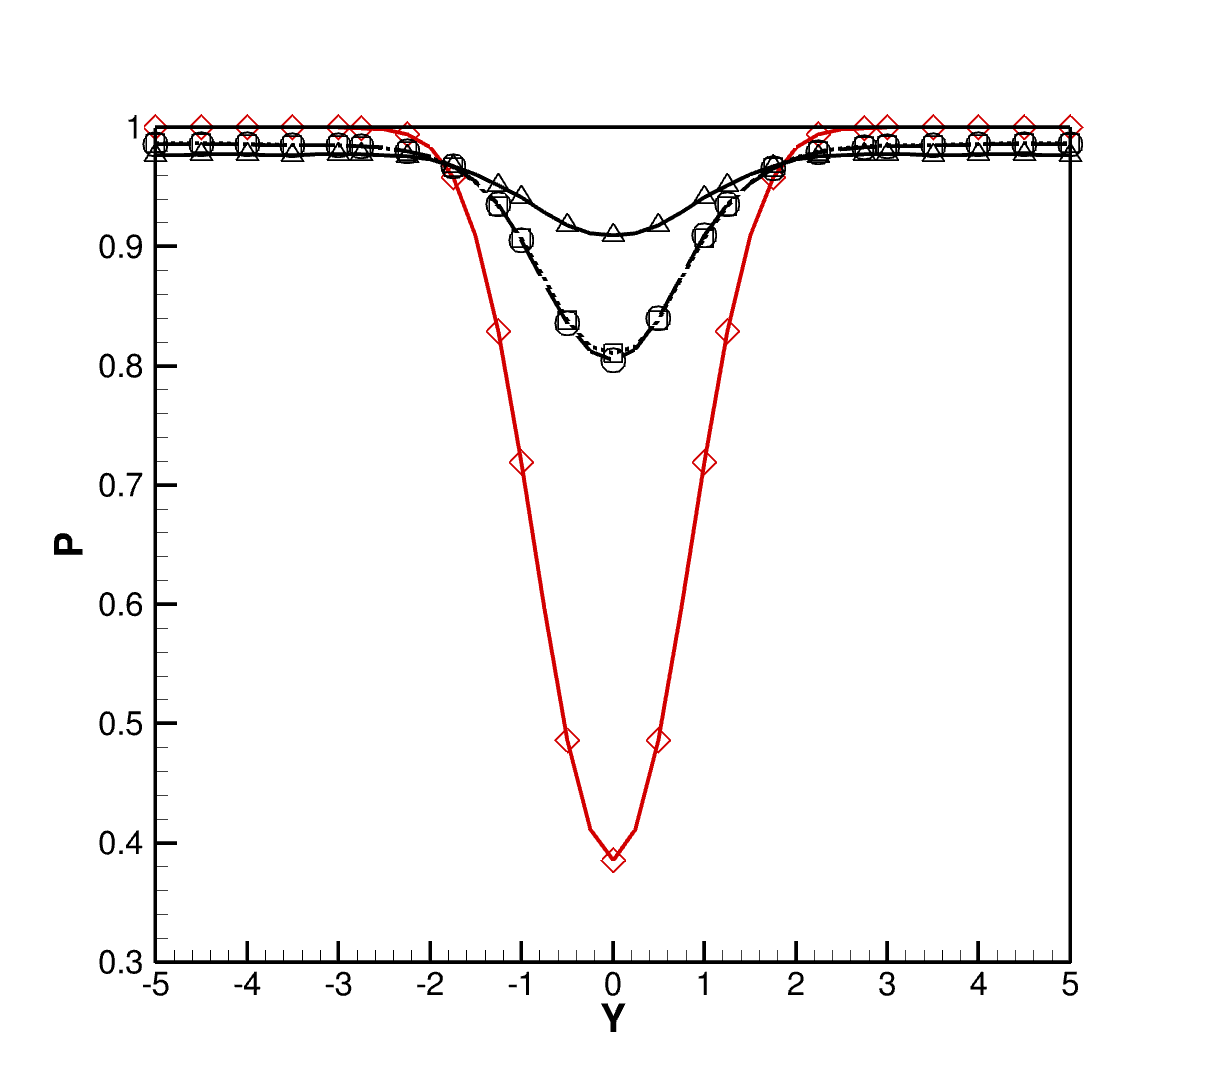
\includegraphics[clip=true, trim= 1.5cm 1.25cm 0.5cm 0.5cm,width=0.325\linewidth]{./figures/vortex3d/03up/03p5}}
     \subfigure[$t=10$ on fine grid]{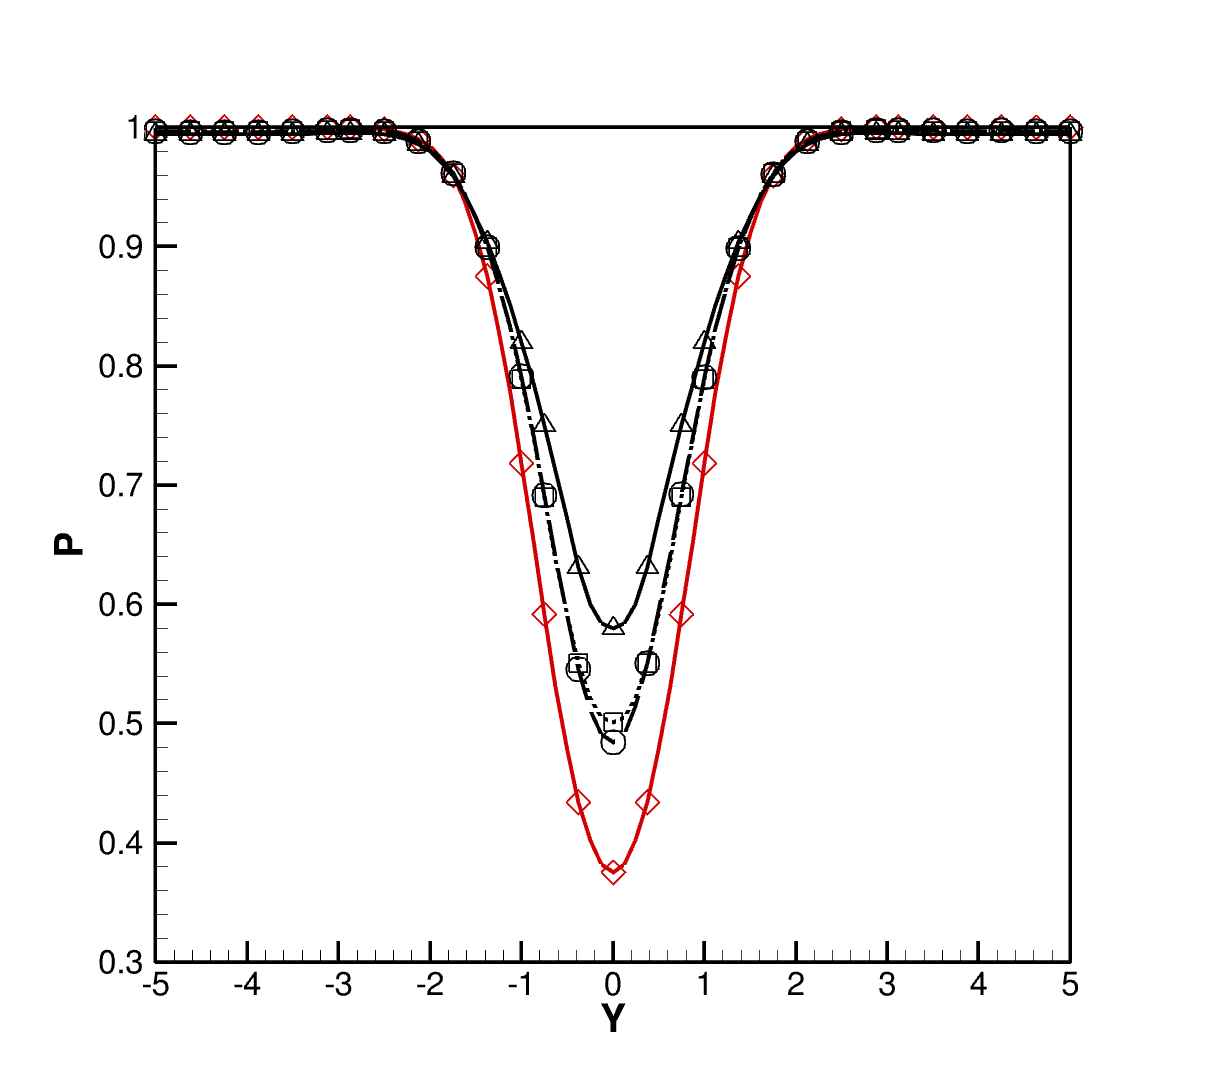
\includegraphics[clip=true, trim= 1.5cm 1.25cm 0.5cm 0.5cm,width=0.325\linewidth]{./figures/vortex3d/05up/05p5}}                   
     \caption{Pressure profiles at $x=0$. (MUSCL: \mline; EDDY: \eline; EDDY-P: \epline; Exact: \exact.)}     
     \label{p135}
\end{figure*}
%%%%%%%%%%%%%%%%%%%%%%%%%%%%%%%%%%%%%%%%%%%%%%%%%%%%%%%%%%%%%%%%
The pressure profiles at $x=0$ and several time instances $t=2$, $t=6$, and $t=10$ are shown in Fig.~\ref{p135}, while the relative $L^{2}$ norms of the error are plotted in Fig.~\ref{l2} (b). The EDDY scheme outperforms the MUSCL scheme, while the EDDY-P scheme demonstrates a slight further improvement, which shows that the modification for the interpolation of pressure is able to further reduce the dissipation. 


The vortex core regions on the medium grid for all schemes are represented by the contour lines of $Q=0$, as shown in Fig.~\ref{q}. As time advances, the vortex core of the MUSCL scheme grows, while that of the EDDY and EDDY-P are maintained, which demonstrates the schemes ability to preserve the vortex due to their lower dissipation.


A study of accuracy was performed for all three schemes on four consecutively refined grids. The $L^{2}$ error of pressure at $t=2$ with respect to the grid spacing is plotted in Fig.~\ref{order}. The slopes of all three schemes are able to match the slope of the referenced 2nd-order line as the grid is refined.
%%%%%%%%%%%%%%%%%%%%%%%%%%%%%%%%%%%%%%%%%%%%%%%%%%%%%%%%%%%%%%%%
\begin{figure}[t]  
\centering
     \subfigure[]{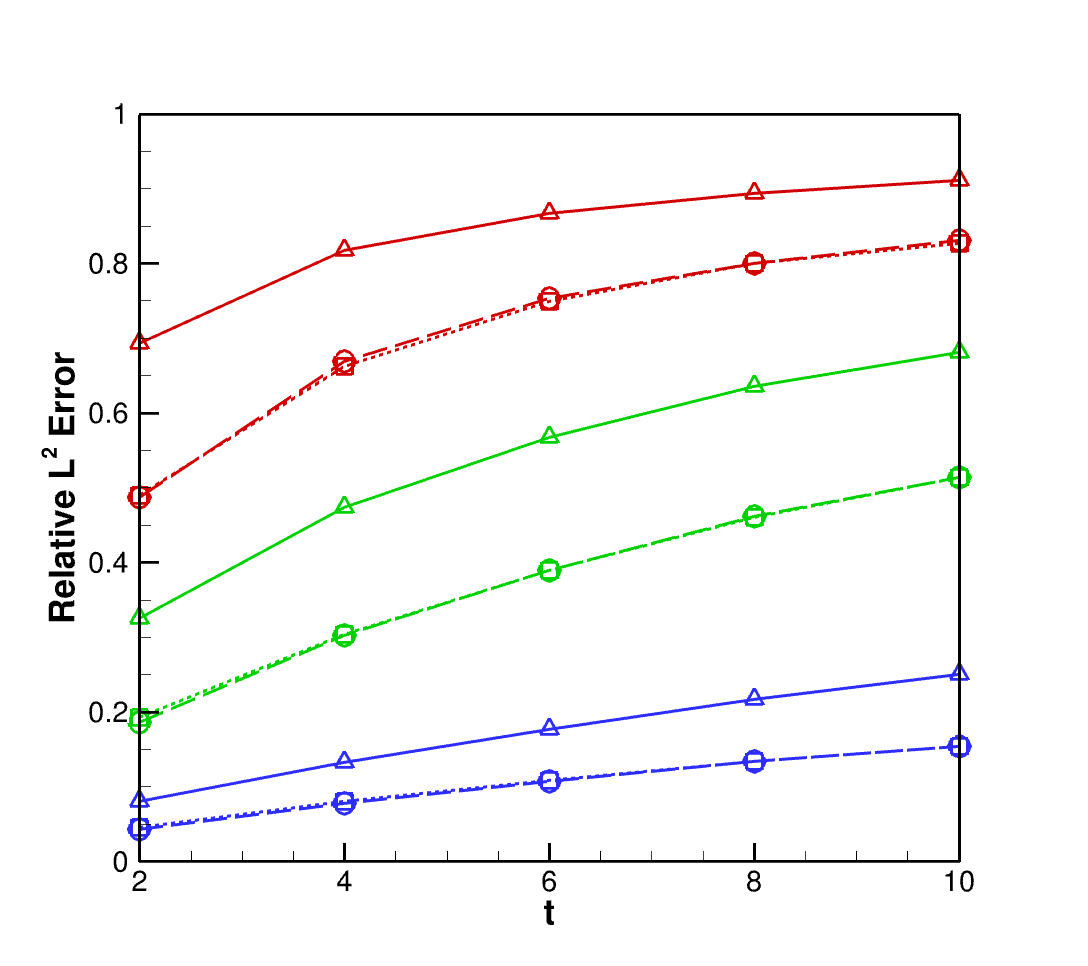
\includegraphics[clip=true, trim= 1.25cm 1.25cm 0.5cm 0.5cm,width=0.49\linewidth]{./figures/vortex3d/l2/u}}              
     \subfigure[]{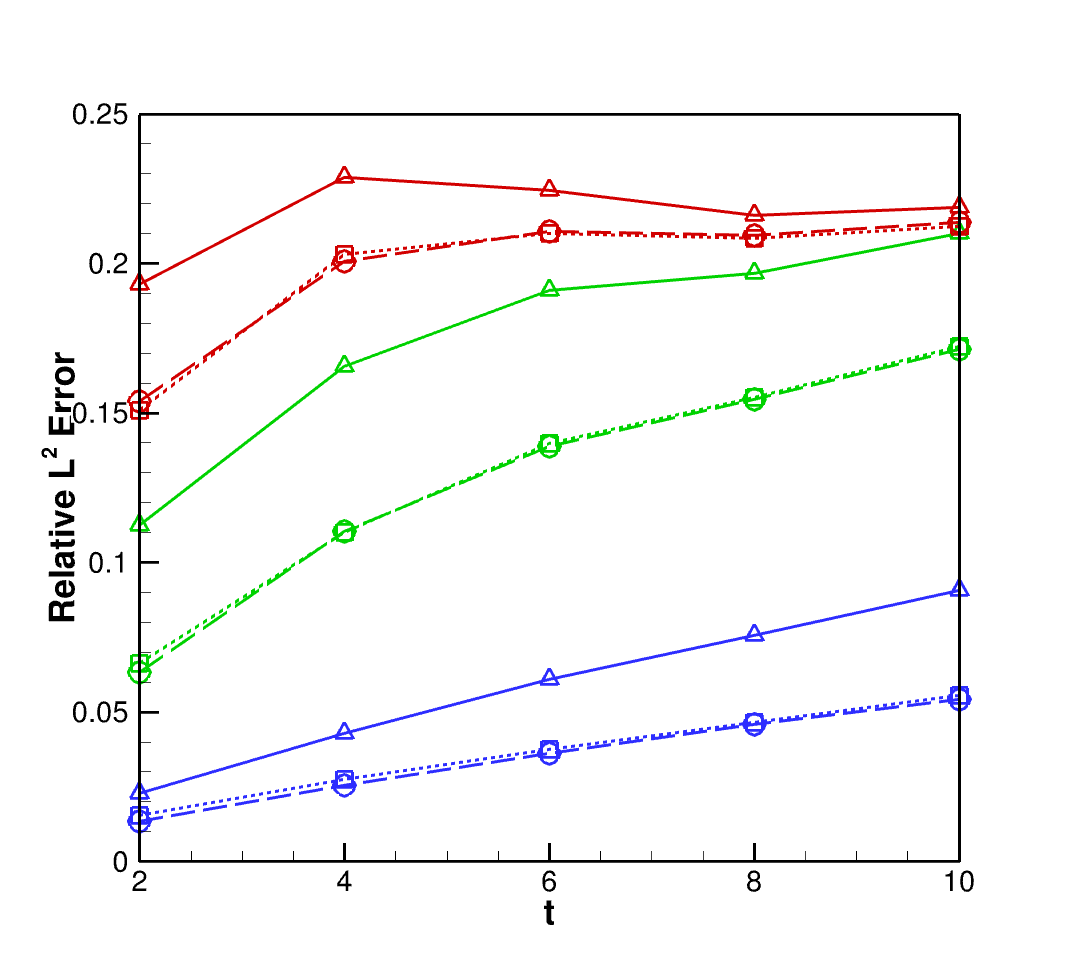
\includegraphics[clip=true, trim= 1.25cm 1.25cm 0.5cm 0.5cm,width=0.49\linewidth]{./figures/vortex3d/l2/p}}                 
     \caption{Relative $L^{2}$ error of (a)velocity (b)pressure. (Coarse grid: MUSCL: \mliner; EDDY: \eliner; EDDY-P: \epliner. Medium grid: MUSCL: \mlineg; EDDY: \elineg; EDDY-P: \eplineg. Fine grid: MUSCL: \mlineb; EDDY: \elineb; EDDY-P: \eplineb.)}
     \label{l2}   
\end{figure}
%%%%%%%%%%%%%%%%%%%%%%%%%%%%%%%%%%%%%%%%%%%%%%%%%%%%%%%%%%%%%%%%
%%%%%%%%%%%%%%%%%%%%%%%%%%%%%%%%%%%%%%%%%%%%%%%%%%%%%%%%%%%%%%%%
%%%%%%%%%%%%%%%%%%%%%%%%%%%%%%%%%%%%%%%%%%%%%%%%%%%%%%%%%%%%%%%%
%%%%%%%%%%%%%%%%%%%%%%%%%%%%%%%%%%%%%%%%%%%%%%%%%%%%%%%%%%%%%%%%
%%%%%%%%%%%%%%%%%%%%%%%%%%%%%%%%%%%%%%%%%%%%%%%%%%%%%%%%%%%%%%%%
%%%%%%%%%%%%%%%%%%%%%%%%%%%%%%%%%%%%%%%%%%%%%%%%%%%%%%%%%%%%%%%%
\begin{figure}[t]  
\centering
     \subfigure[]{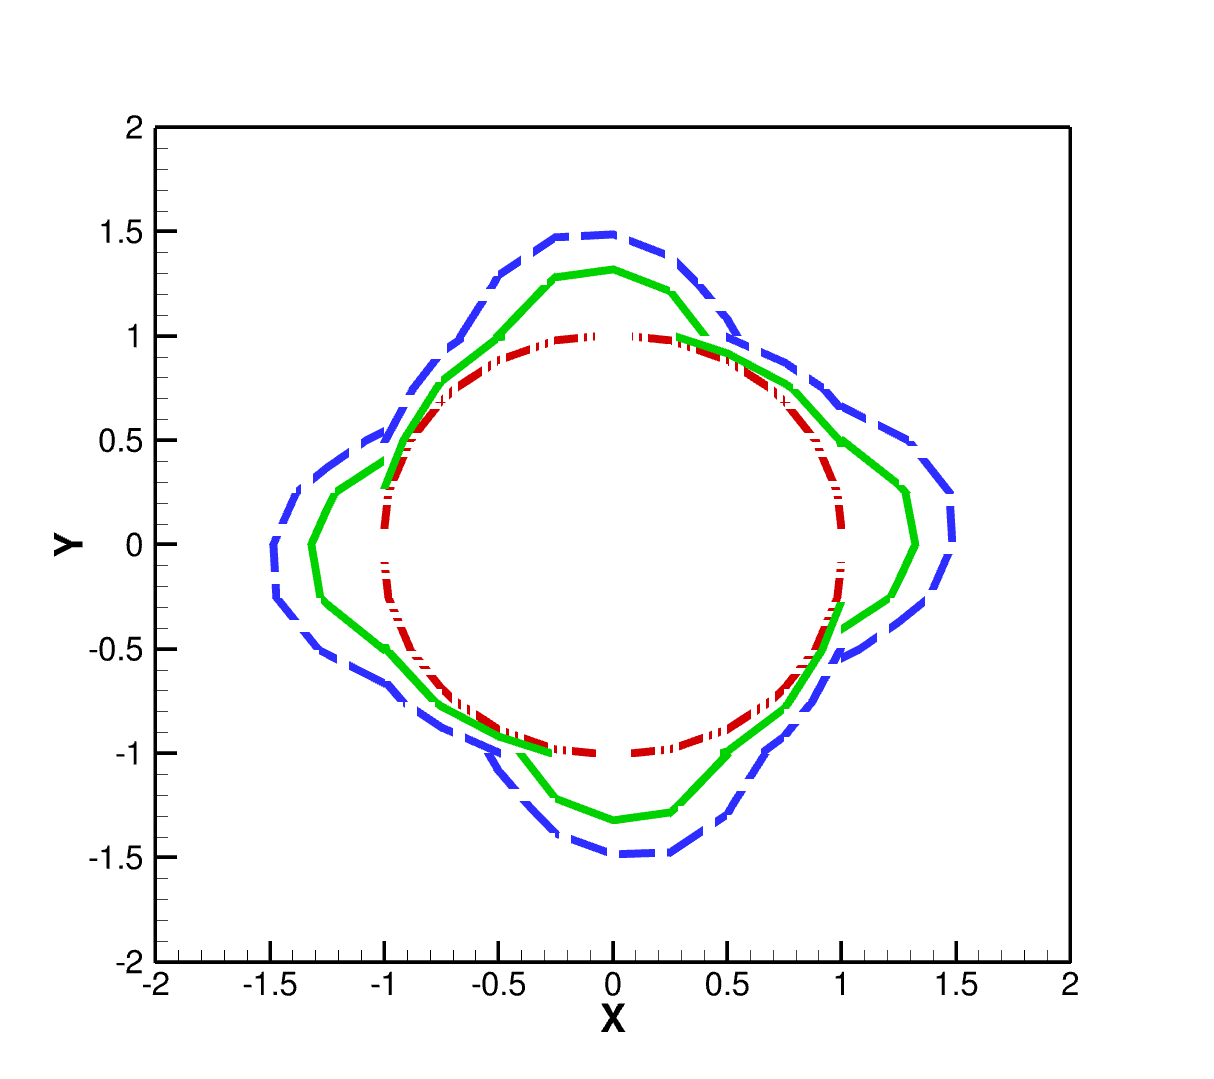
\includegraphics[clip=true, trim= 1.5cm 1.25cm 0.5cm 0.5cm,width=0.325\linewidth]{./figures/vortex3d/lines/m}}              
     \subfigure[]{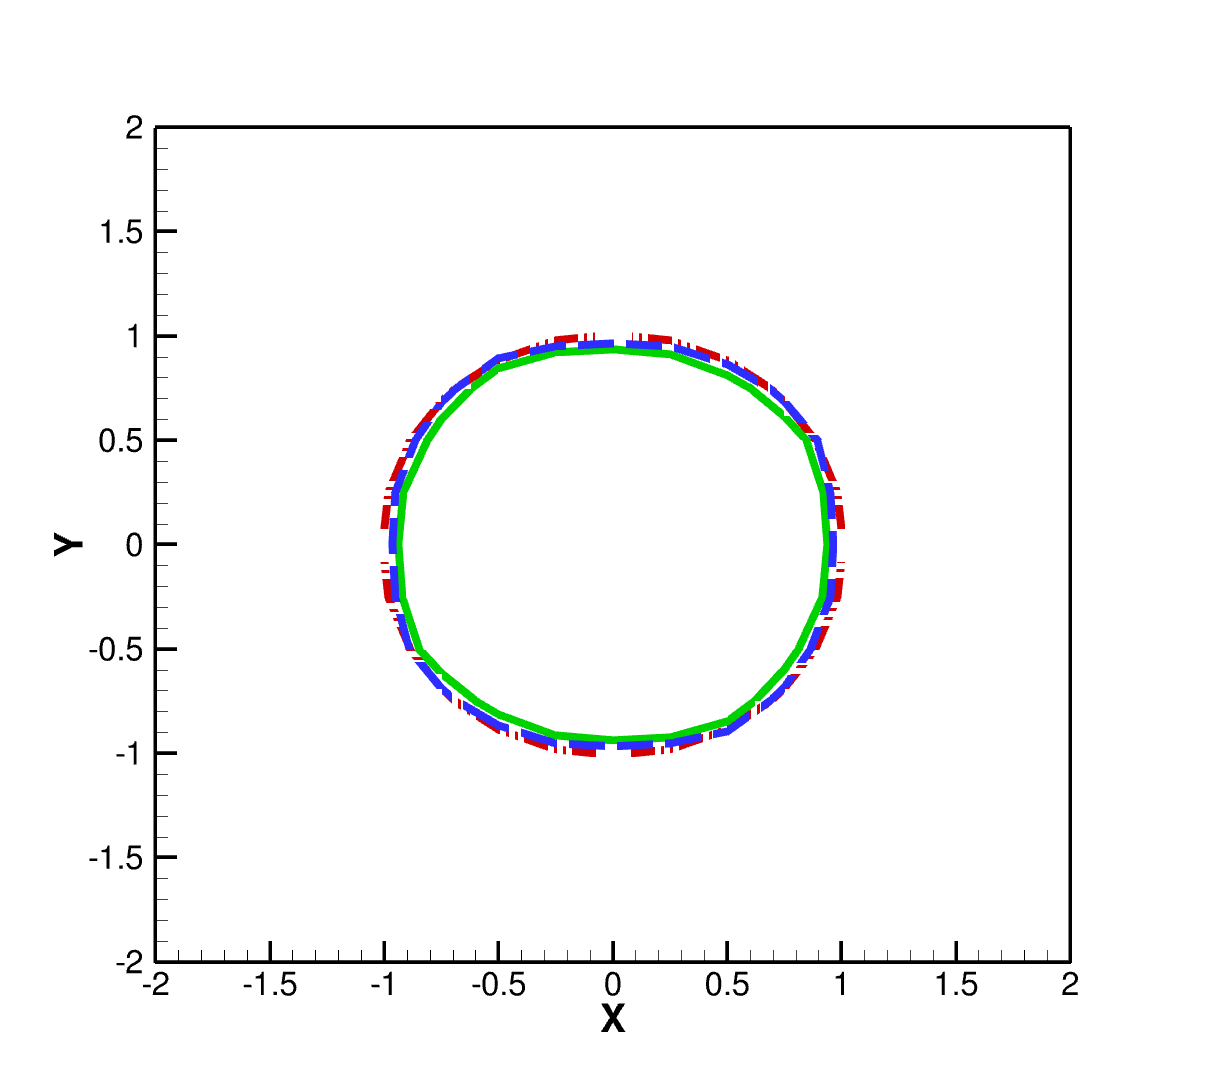
\includegraphics[clip=true, trim= 1.5cm 1.25cm 0.5cm 0.5cm,width=0.325\linewidth]{./figures/vortex3d/lines/e}}
     \subfigure[]{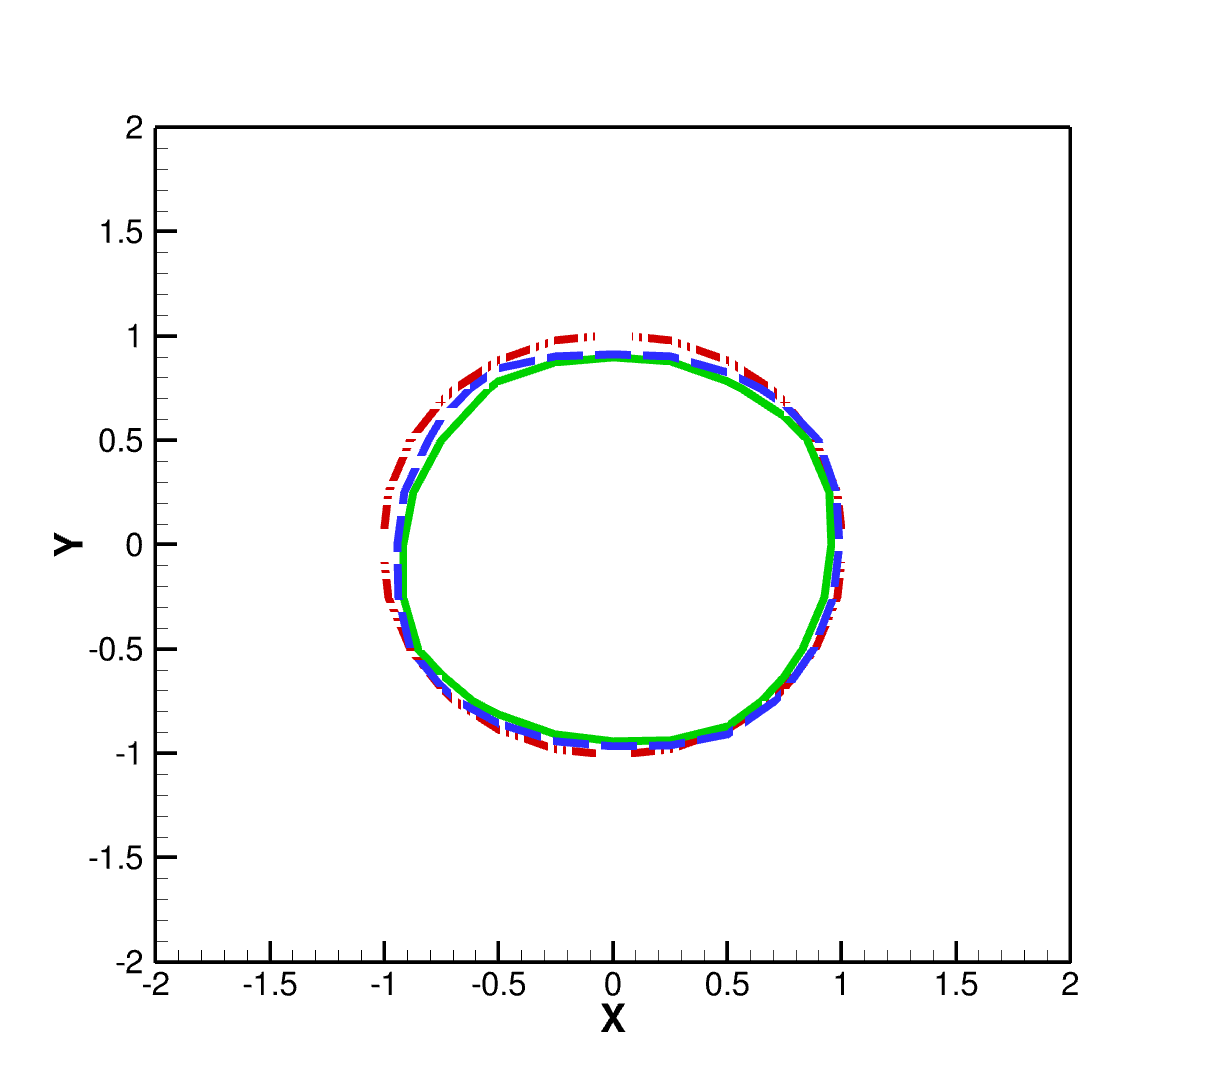
\includegraphics[clip=true, trim= 1.5cm 1.25cm 0.5cm 0.5cm,width=0.325\linewidth]{./figures/vortex3d/lines/ep}}                    
     \caption{$Q=0$ contour lines on medium grid for (a)MUSCL (b)EDDY (c)EDDY-P schemes. ($t=0$: \redline; $t=4$: \greenline; $t=8$: \blueline.)}
     \label{q}   
\end{figure}
%%%%%%%%%%%%%%%%%%%%%%%%%%%%%%%%%%%%%%%%%%%%%%%%%%%%%%%%%%%%%%%%
%%%%%%%%%%%%%%%%%%%%%%%%%%%%%%%%%%%%%%%%%%%%%%%%%%%%%%%%%%%%%%%%
%%%%%%%%%%%%%%%%%%%%%%%%%%%%%%%%%%%%%%%%%%%%%%%%%%%%%%%%%%%%%%%%
\begin{figure}[t]  
\centering
     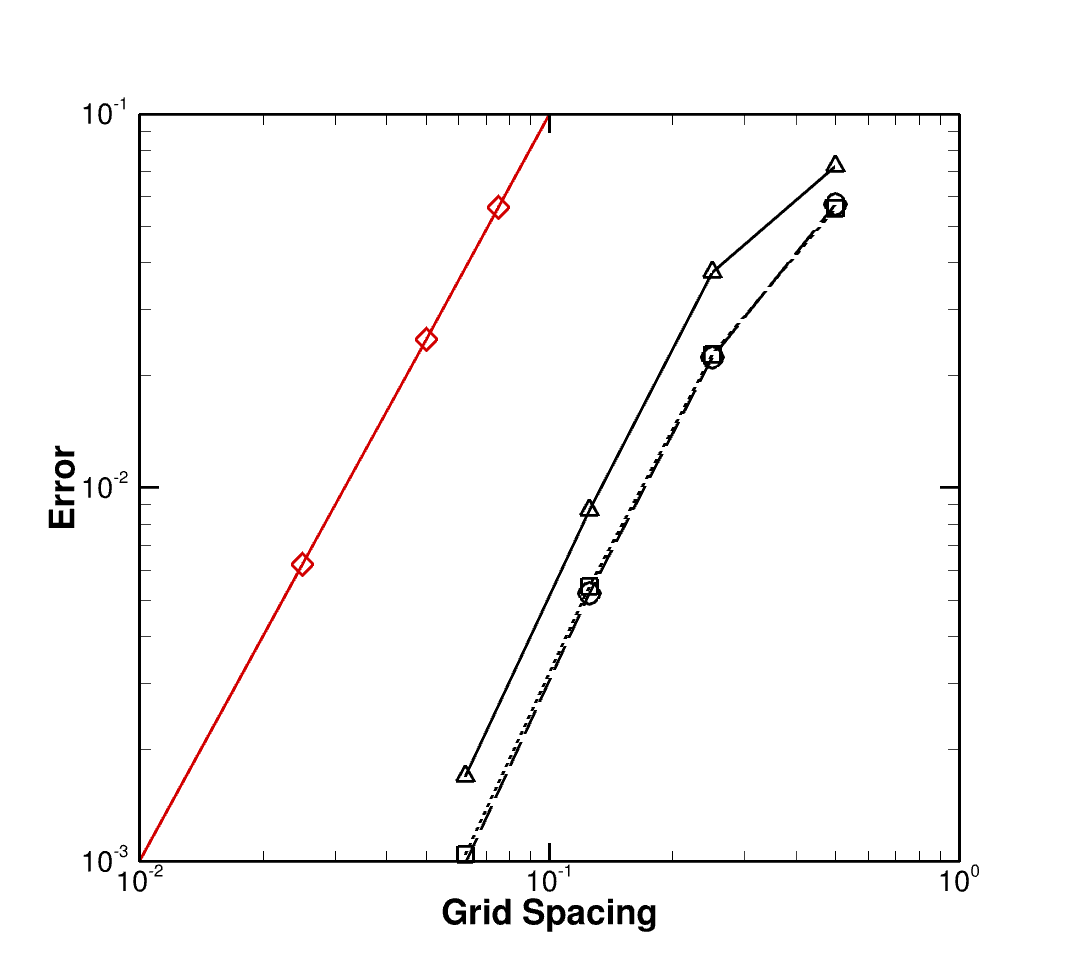
\includegraphics[clip=true, trim= 1.5cm 1.25cm 0.5cm 0.5cm,width=0.99\linewidth]{./figures/vortex3d/order}                            
     \caption{Accuracy study of different schemes. (MUSCL: \mline; EDDY: \eline; EDDY-P: \epline; 2nd-order: \exact.)}
     \label{order}   
\end{figure}















\subsection{Three Dimensional Viscous Vortex Advection}
A viscous vortex advection case is performed on a grid, where $\Delta x=\Delta y=\Delta z=0.25$ and $-5\le x \le5$, $-5\le y \le 5$, and $0\le z \le 24$. A vortex profile is fixed at the inlet, where the density and velocity profiles are prescribed according to Eqn.~\ref{vor-equ}, and the pressure is set to be constant at the outlet. Periodic boundary conditions are imposed for the remaining boundaries. The Reynolds number is set to $1.56\times10^6$. The vortex is expected to be dissipated in the stream-wise more severely than the inviscid cases, and the isosurface of vorticity magnitude would resemble a cone.

The test cases are simulated with the baseline MUSCL scheme, the original and the extended eddy-preserving limiter schemes. The unsteady simulations for all schemes start from a converged steady solution computed from the MUSCL scheme. The time step is set to be constant $\Delta t=0.04$, and at final time $t=20$, all simulations have reached quasi-steady states.

The vorticity contours at several stream-wise locations are plotted in Fig. \ref{vortv}. At each location, the EDDY and EDDY-P schemes produce higher vorticity magnitude in the central region than the MUSCL scheme. The isosurface of vorticity with magnitude unity is plotted in Fig. \ref{iso} to illustrate the vortex. The EDDY and EDDY-P schemes are able to preserve the vortex considerably longer than the MUSCL scheme. The comparisons demonstrate that the EDDY and EDDY-P schemes also outperform the MUSCL scheme for the benchmark turbulent flow simulation.
%%%%%%%%%%%%%%%%%%%%%%%%%%%%%%%%%%%%%%%%%%%%%%%%%%%%%%%%%%%%%%%%
%%%%%%%%%%%%%%%%%%%%%%%%%%%%%%%%%%%%%%%%%%%%%%%%%%%%%%%%%%%%%%%%
\begin{figure}[t]  
\centering
     \subfigure[MUSCL at $z=1$]{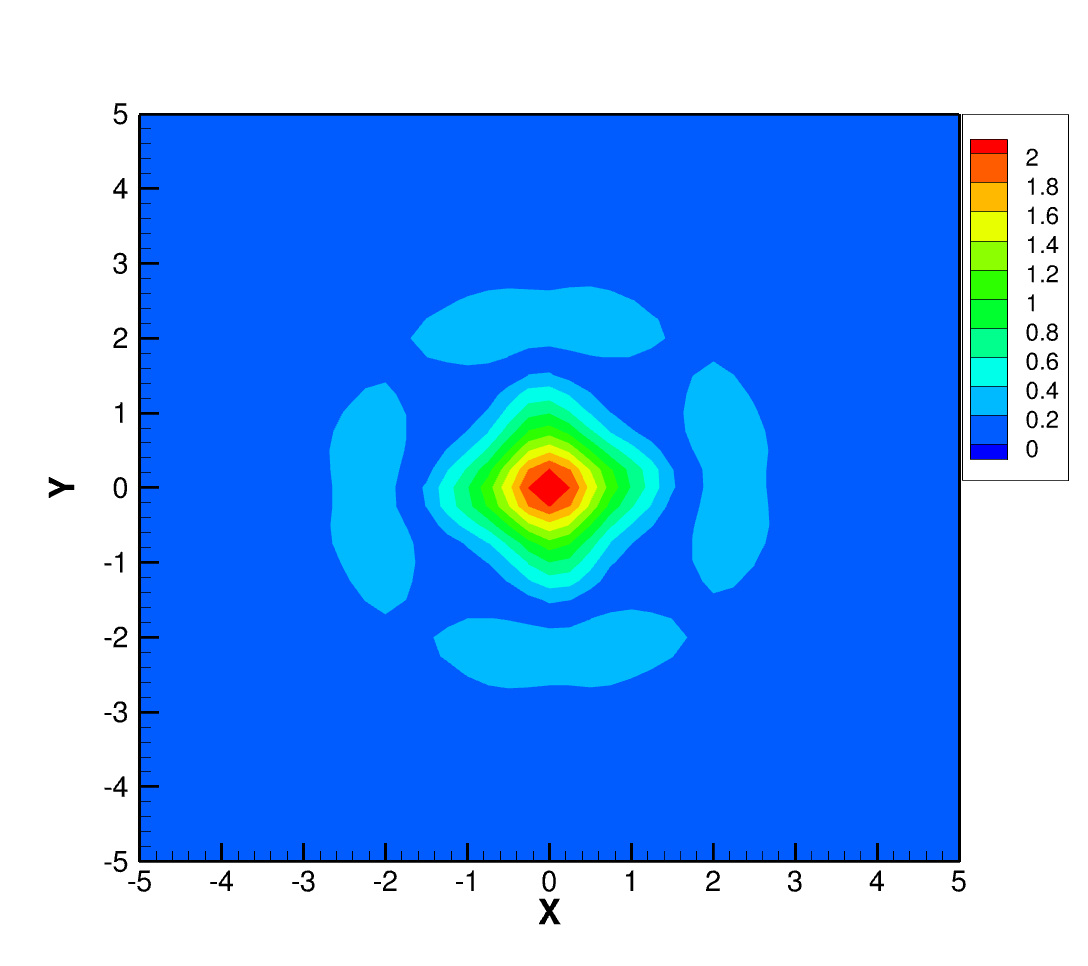
\includegraphics[clip=true, trim= 1.5cm 1.25cm 0.25cm 0.5cm,width=0.325\linewidth]{./figures/vortex3d/viscous/m1}}              
     \subfigure[EDDY at $z=1$]{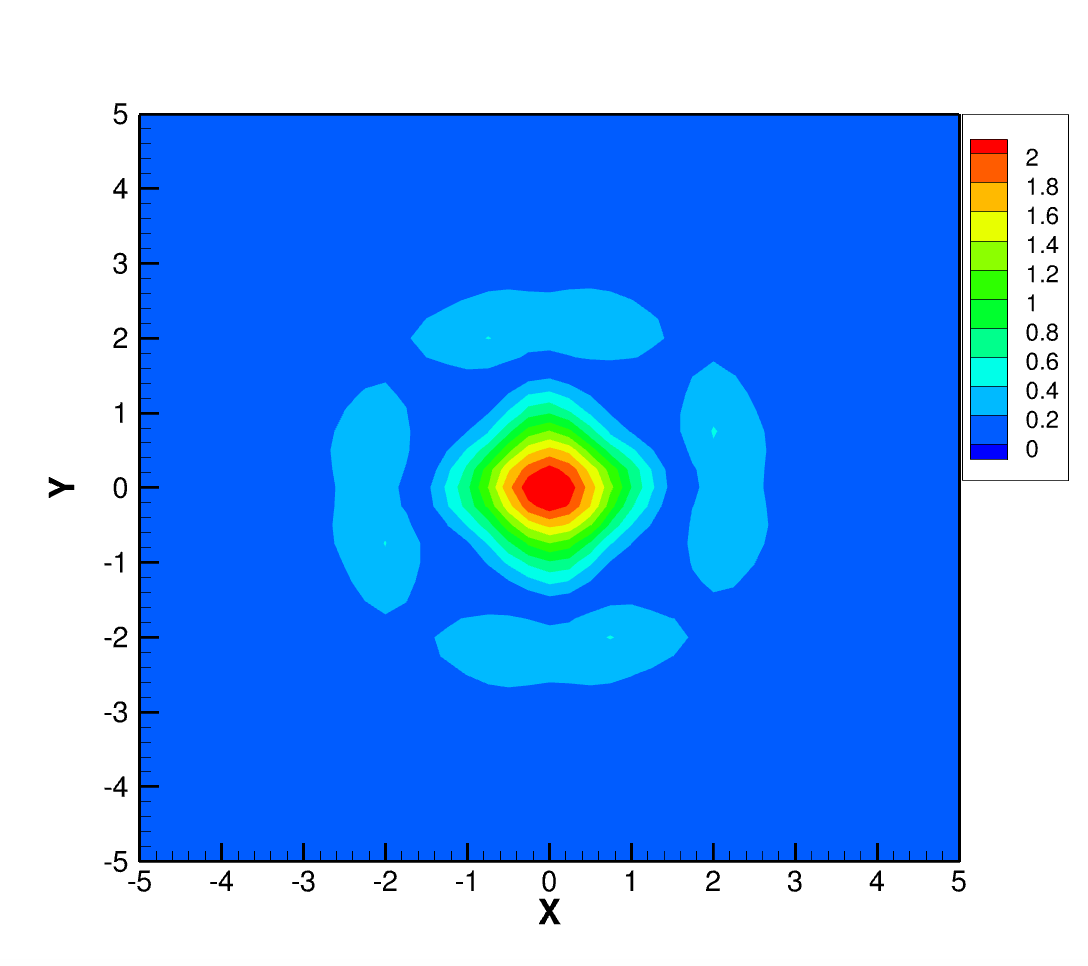
\includegraphics[clip=true, trim= 1.5cm 1.25cm 0.25cm 0.5cm,width=0.325\linewidth]{./figures/vortex3d/viscous/e1}}
     \subfigure[EDDY-P at $z=1$]{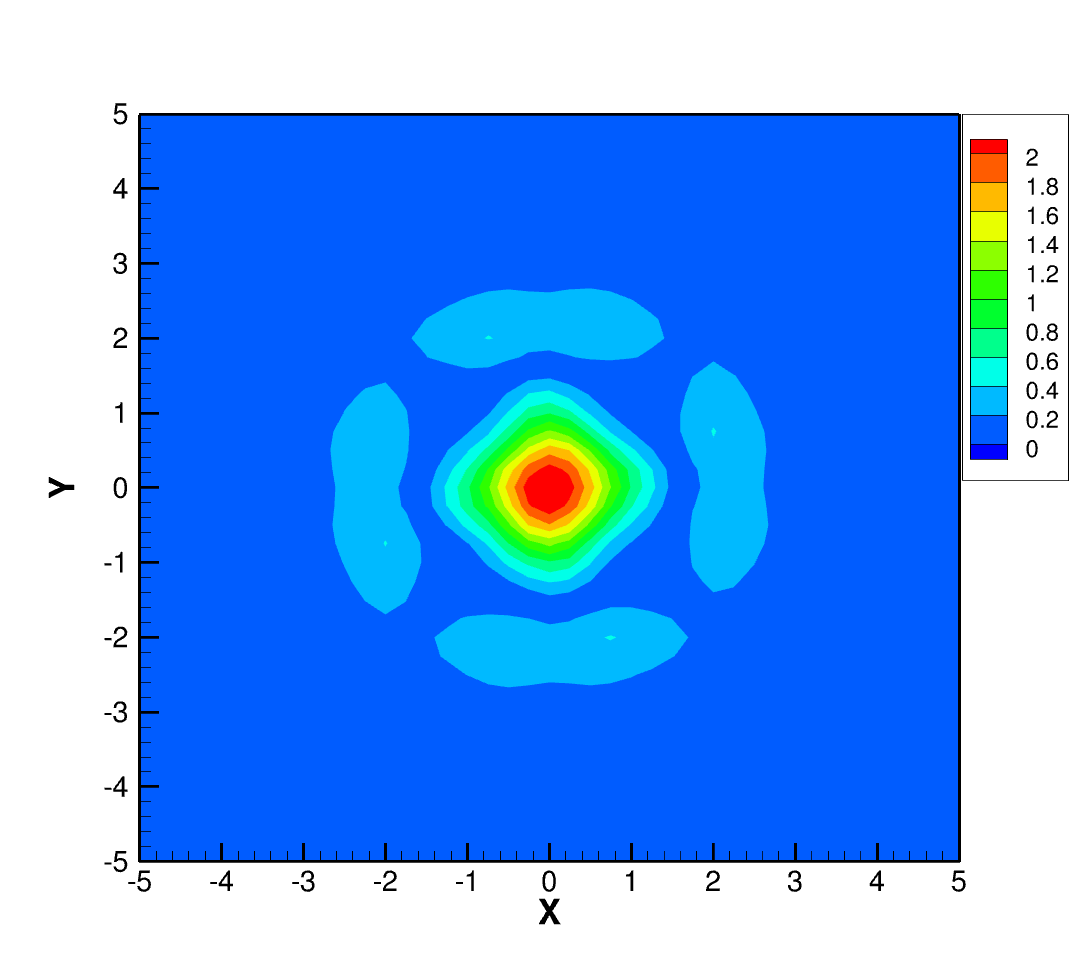
\includegraphics[clip=true, trim= 1.5cm 1.25cm 0.25cm 0.5cm,width=0.325\linewidth]{./figures/vortex3d/viscous/ep1}}
     \subfigure[MUSCL at $z=2$]{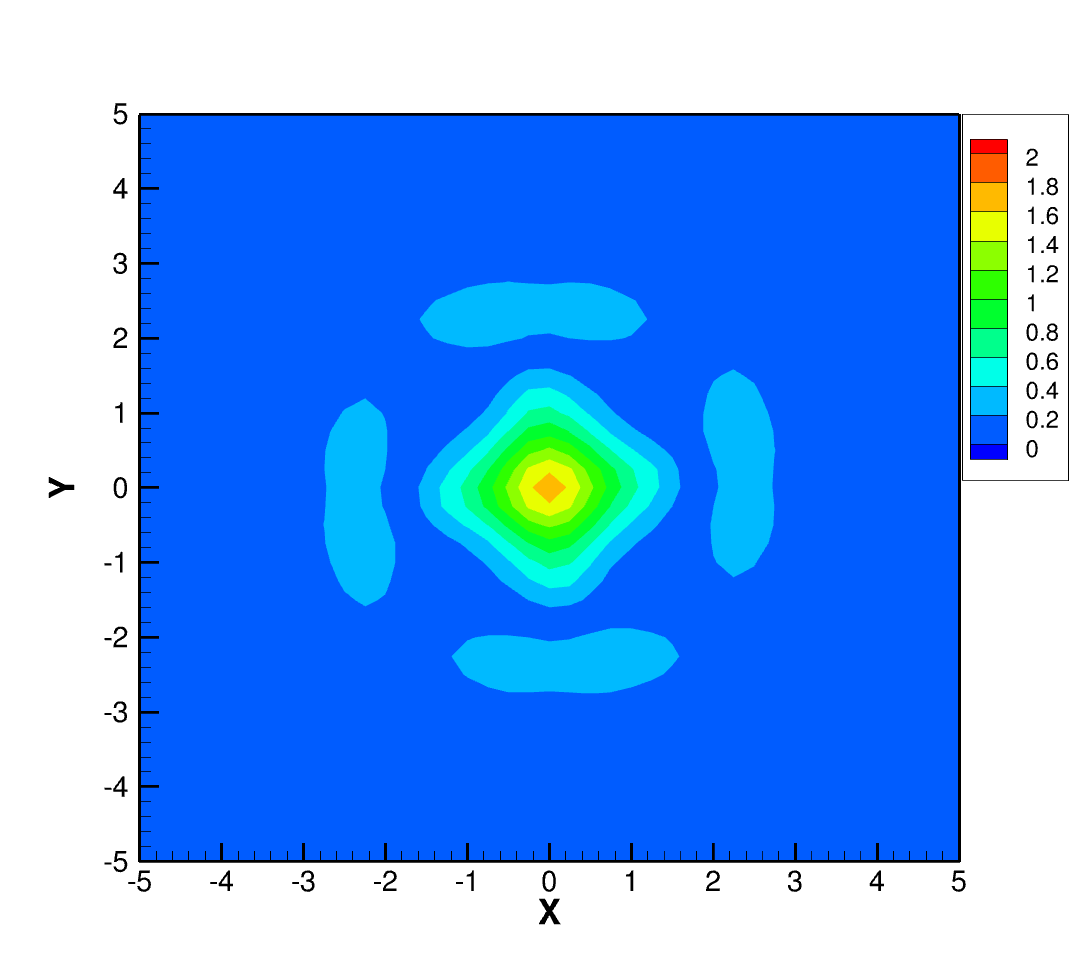
\includegraphics[clip=true, trim= 1.5cm 1.25cm 0.25cm 0.5cm,width=0.325\linewidth]{./figures/vortex3d/viscous/m2}}              
     \subfigure[EDDY at $z=2$]{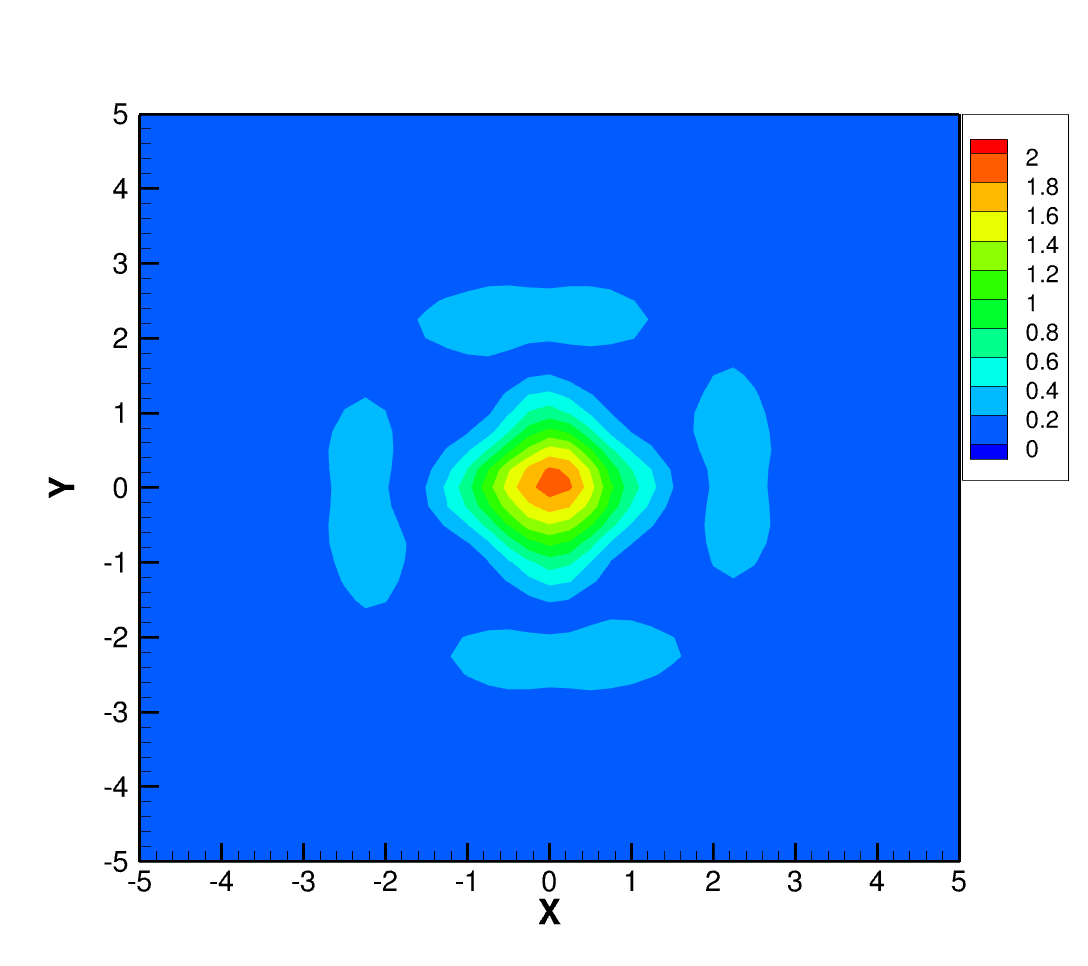
\includegraphics[clip=true, trim= 1.5cm 1.25cm 0.25cm 0.5cm,width=0.325\linewidth]{./figures/vortex3d/viscous/e2}}
     \subfigure[EDDY-P at $z=2$]{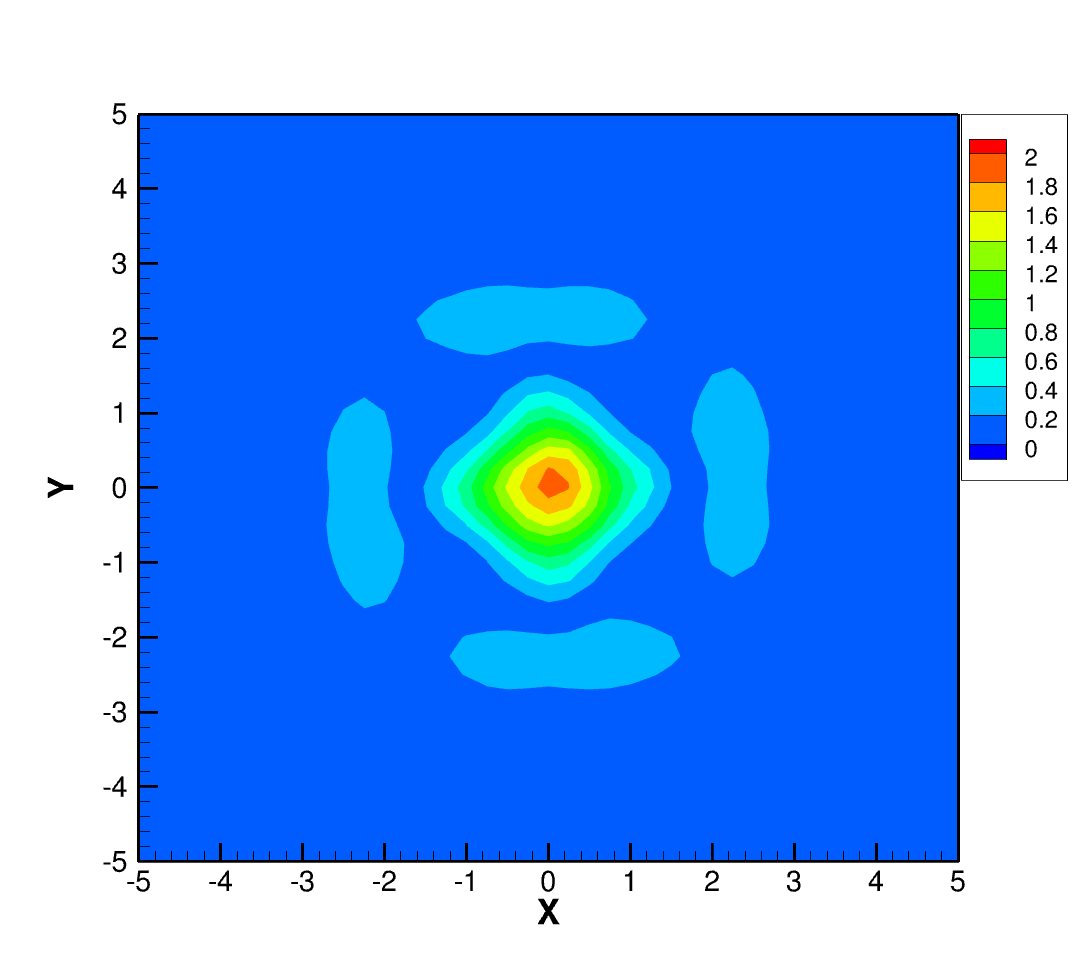
\includegraphics[clip=true, trim= 1.5cm 1.25cm 0.25cm 0.5cm,width=0.325\linewidth]{./figures/vortex3d/viscous/ep2}} 
     \subfigure[MUSCL at $z=3$]{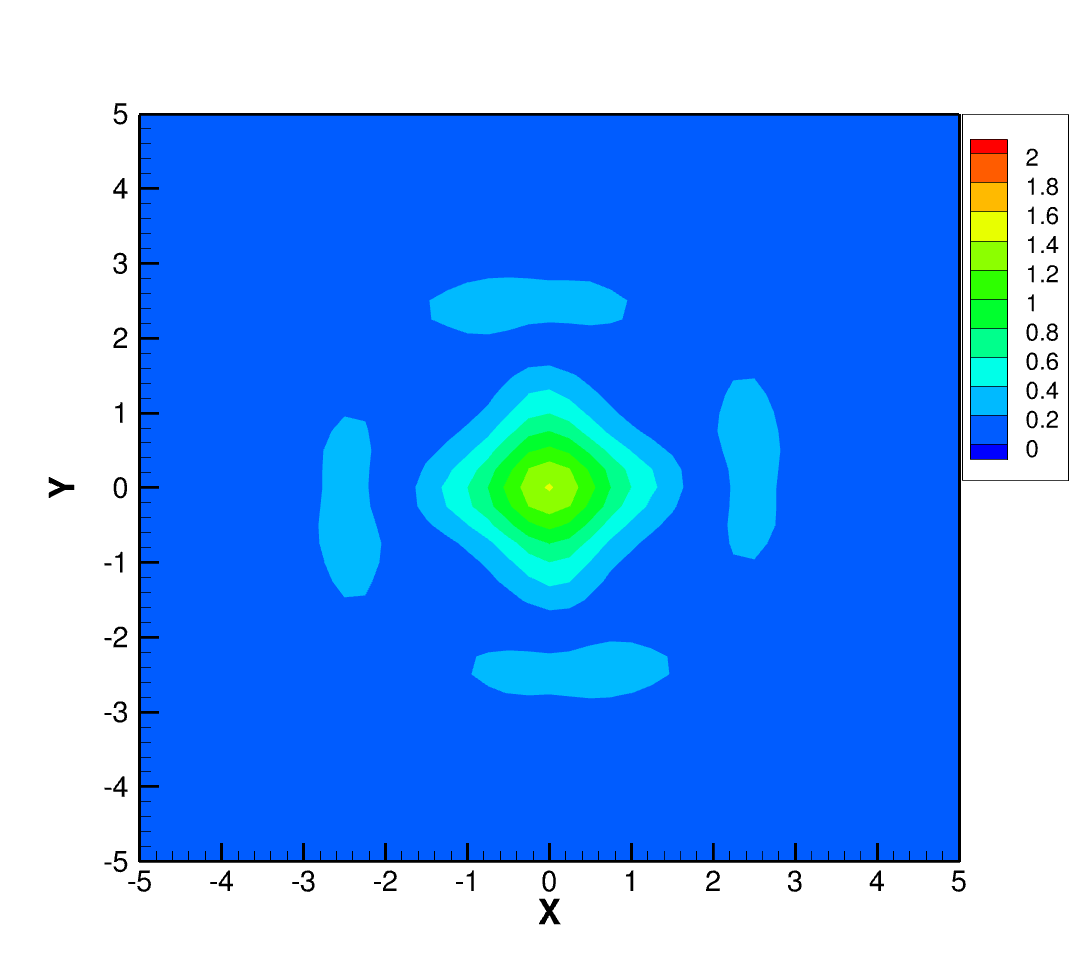
\includegraphics[clip=true, trim= 1.5cm 1.25cm 0.25cm 0.5cm,width=0.325\linewidth]{./figures/vortex3d/viscous/m3}}              
     \subfigure[EDDY at $z=3$]{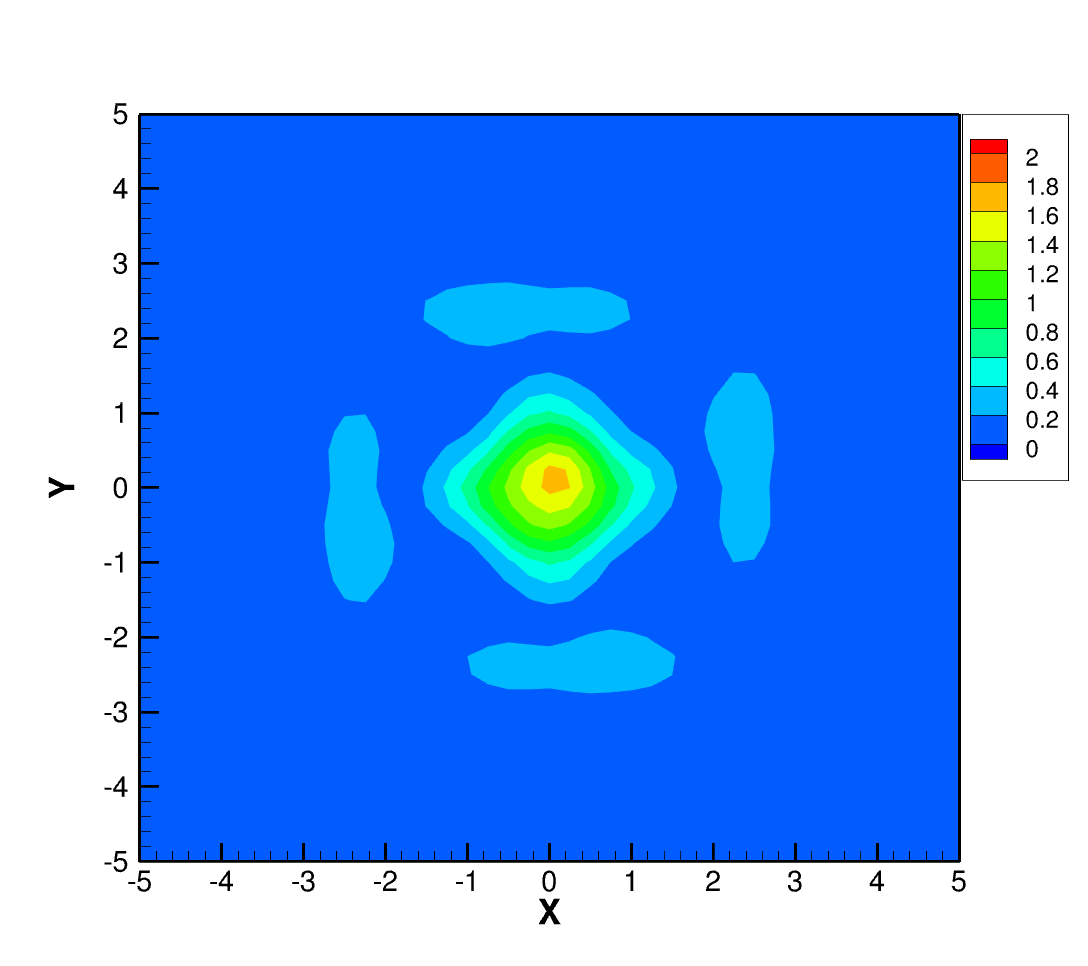
\includegraphics[clip=true, trim= 1.5cm 1.25cm 0.25cm 0.5cm,width=0.325\linewidth]{./figures/vortex3d/viscous/e3}}
     \subfigure[EDDY-P at $z=3$]{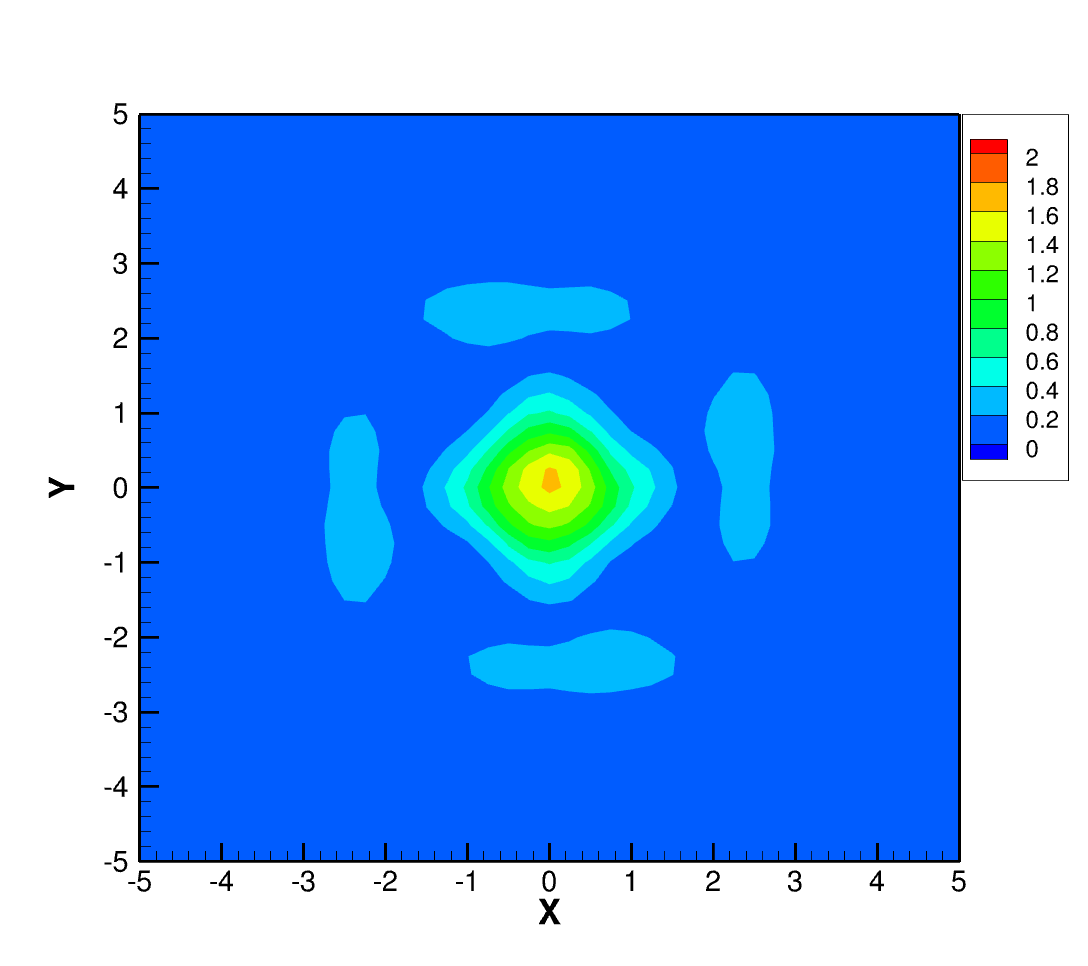
\includegraphics[clip=true, trim= 1.5cm 1.25cm 0.25cm 0.5cm,width=0.325\linewidth]{./figures/vortex3d/viscous/ep3}}                               
     \caption{Vorticity contours at different locations for three schemes.}
     \label{vortv}
\end{figure}
%%%%%%%%%%%%%%%%%%%%%%%%%%%%%%%%%%%%%%%%%%%%%%%%%%%%%%%%%%%%%%%%
%%%%%%%%%%%%%%%%%%%%%%%%%%%%%%%%%%%%%%%%%%%%%%%%%%%%%%%%%%%%%%%%
%%%%%%%%%%%%%%%%%%%%%%%%%%%%%%%%%%%%%%%%%%%%%%%%%%%%%%%%%%%%%%%%
%\begin{figure}[t]  
%\centering
%     \subfigure[]{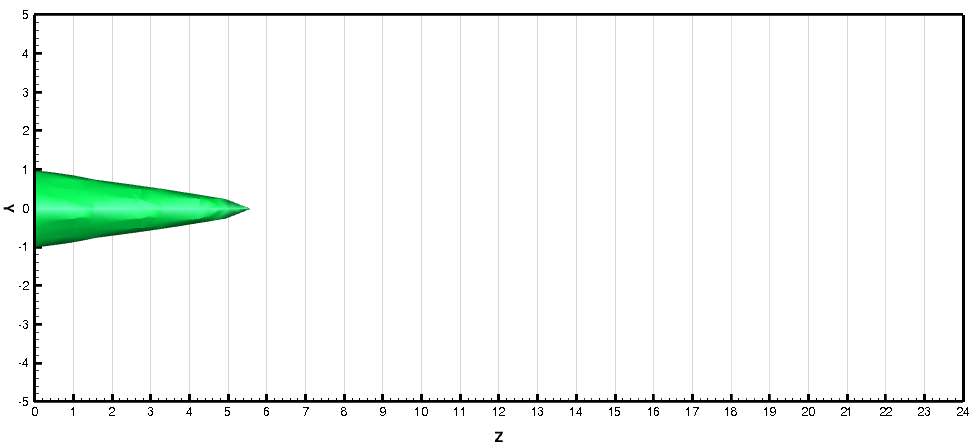
\includegraphics[clip=true, trim= 0.0cm 0.0cm 0.0cm 0.0cm,width=0.99\linewidth]{./figures/vortex3d/viscous/1}}               
%     \subfigure[]{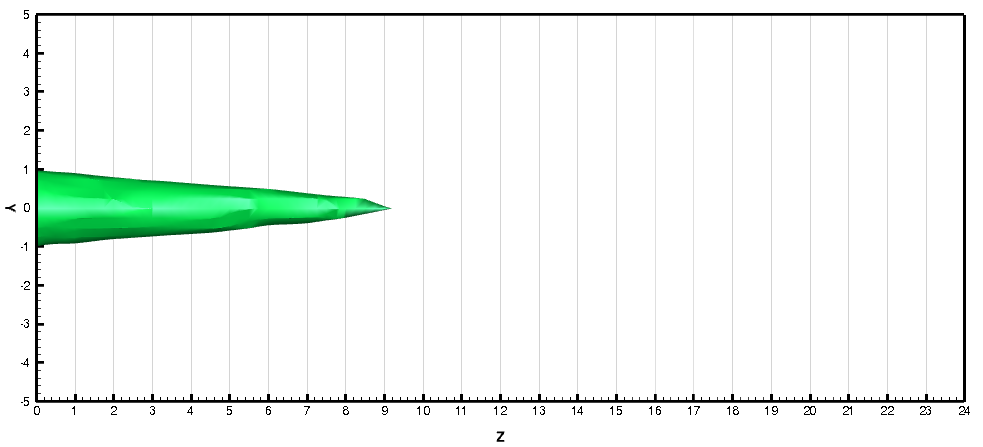
\includegraphics[clip=true, trim= 0.0cm 0.0cm 0.0cm 0.0cm,width=0.99\linewidth]{./figures/vortex3d/viscous/2}} 
%     \subfigure[]{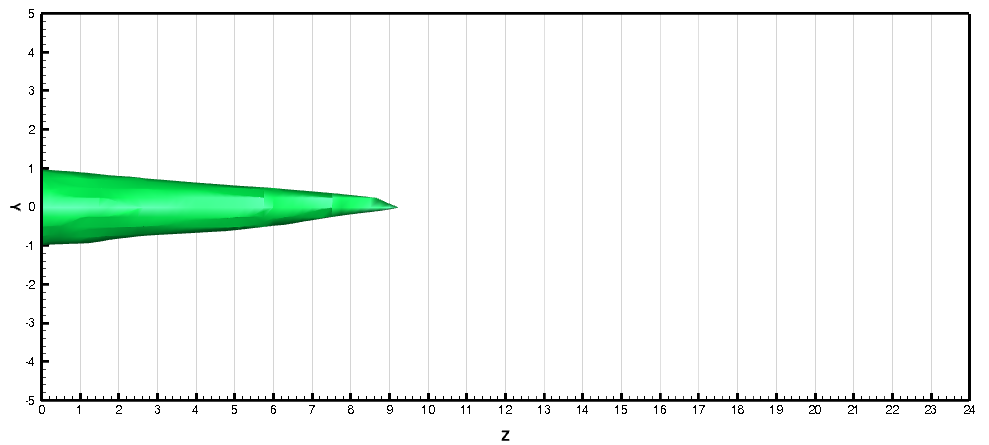
\includegraphics[clip=true, trim= 0.0cm 0.0cm 0.0cm 0.0cm,width=0.99\linewidth]{./figures/vortex3d/viscous/3}}               
%     \caption{Isosurface of vorticity magnitude computed by three schemes at $t=20$. (a)MUSCL (b)EDDY (c)EDDY-P.}
%     \label{iso}
%\end{figure}
%%%%%%%%%%%%%%%%%%%%%%%%%%%%%%%%%%%%%%%%%%%%%%%%%%%%%%%%%%%%%%%%
%%%%%%%%%%%%%%%%%%%%%%%%%%%%%%%%%%%%%%%%%%%%%%%%%%%%%%%%%%%%%%%%
%%%%%%%%%%%%%%%%%%%%%%%%%%%%%%%%%%%%%%%%%%%%%%%%%%%%%%%%%%%%%%%%
\begin{figure*}[t]  
\centering
     \subfigure[]{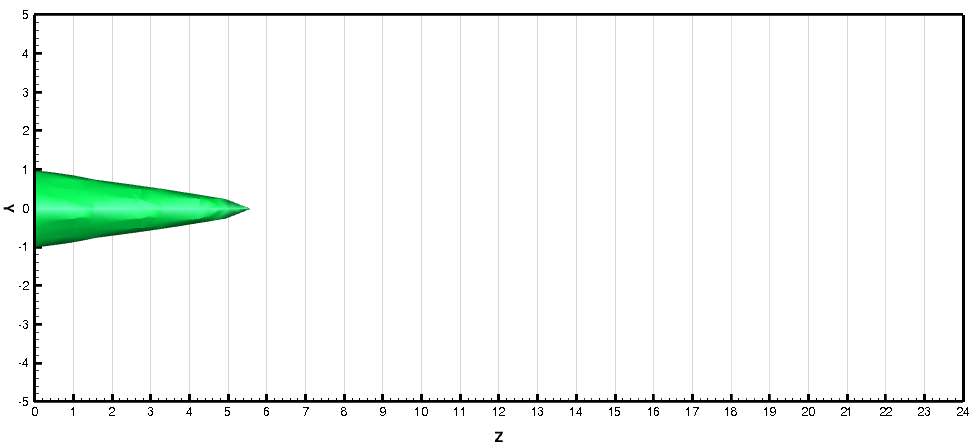
\includegraphics[clip=true, trim= 0.0cm 0.0cm 0.0cm 0.0cm,width=0.325\linewidth]{./figures/vortex3d/viscous/1}}               
     \subfigure[]{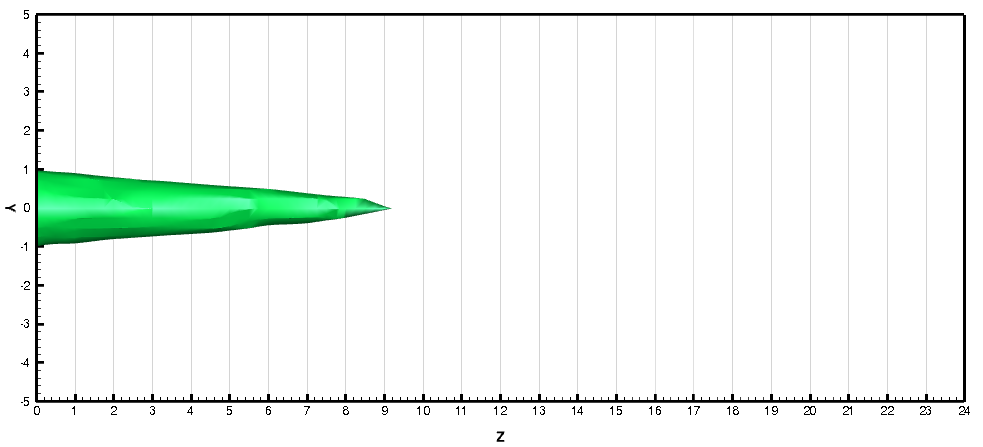
\includegraphics[clip=true, trim= 0.0cm 0.0cm 0.0cm 0.0cm,width=0.325\linewidth]{./figures/vortex3d/viscous/2}} 
     \subfigure[]{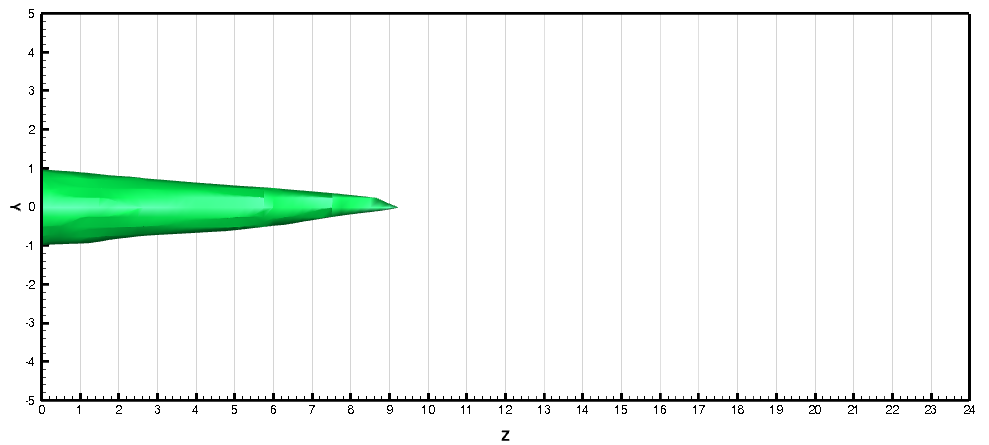
\includegraphics[clip=true, trim= 0.0cm 0.0cm 0.0cm 0.0cm,width=0.325\linewidth]{./figures/vortex3d/viscous/3}}               
     \caption{Isosurface of vorticity magnitude computed by three schemes at $t=20$. (a)MUSCL (b)EDDY (c)EDDY-P.}
     \label{iso}
\end{figure*}




\subsection{BulbT Test Case}
The BulbT project was initiated at the ``Laboratoire de Machines Hydrauliques'' (LAMH) of Laval University, and aimed at investigating the flow phenomena in a bulb turbine \cite{vu2014cfd}. The turbine model consists of an intake, a bulb and a draft tube, as illustrated in Fig.~\ref{bulbt}. 
%%%%%%%%%%%%%%%%%%%%%%%%%%%%%%%%%%%%%%%%%%%%%%%%%%%%%%%%%%%
\begin{figure}[t]  
\centering
     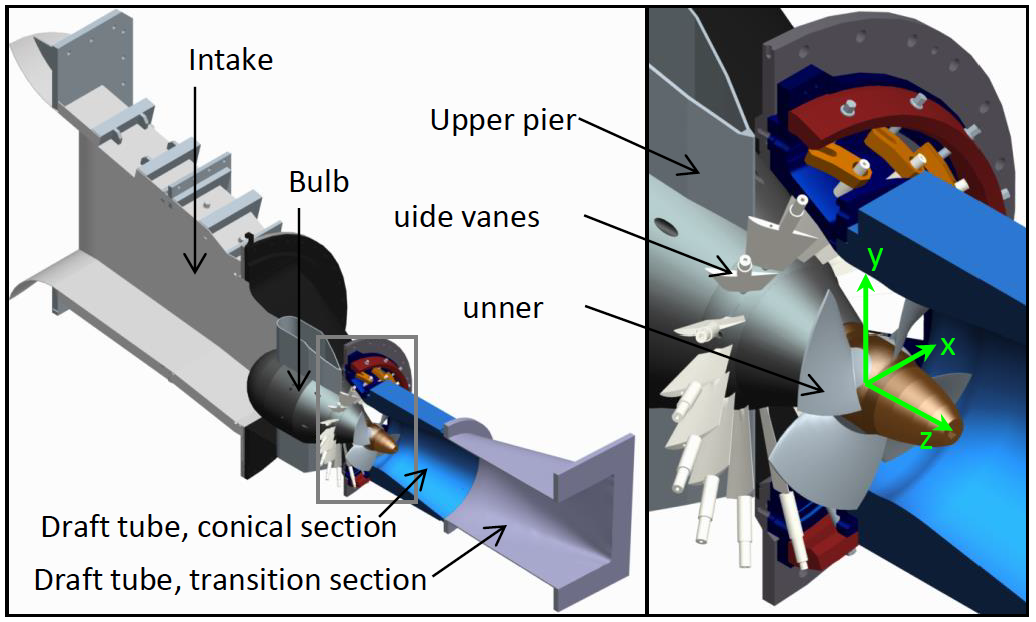
\includegraphics[clip=true, trim= 0.0cm 0.0cm 0.0cm 0.0cm,width=0.99\linewidth]{./figures/bulbt/bulbt}                            
     \caption{Turbine model of BulbT \cite{vuillemard2014experimental}.}
     \label{bulbt}
\end{figure} 
%%%%%%%%%%%%%%%%%%%%%%%%%%%%%%%%%%%%%%%%%%%%%%%%%%%%%%%%%%%
\begin{figure}[t] 
\centering
     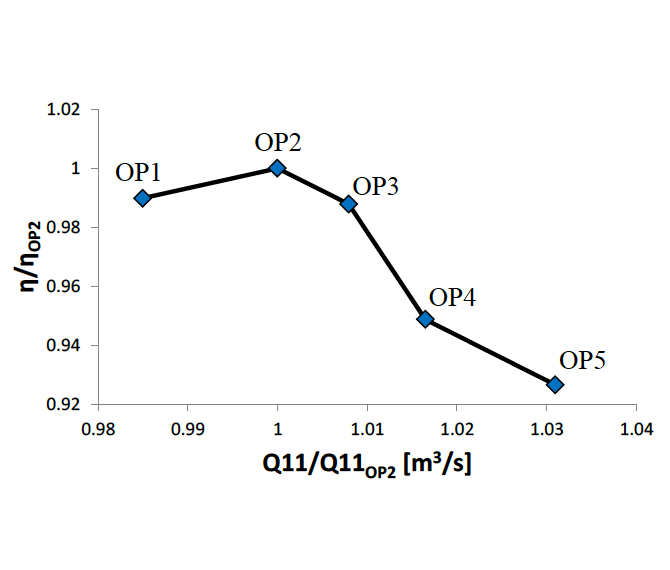
\includegraphics[clip=true, trim= 0.0cm 3.0cm 0.0cm 3.0cm,width=0.99\linewidth]{./figures/bulbt/bulbt-op}                  
     \caption{Operating points of BulbT \cite{vuillemard2014experimental}.}
     \label{bulbt-op}
\end{figure}
%%%%%%%%%%%%%%%%%%%%%%%%%%%%%%%%%%%%%%%%%%%%%%%%%%%%%%%%%%%
%%%%%%%%%%%%%%%%%%%%%%%%%%%%%%%%%%%%%%%%%%%%%%%%%%%%%%%%%%%

The experiments were conducted at five Operating Points (OP) as shown in Fig.~\ref{bulbt-op}. OP2 is the one closest to the best efficiency point, and the flow phenomenon is less complex compared to other OPs. Therefore, in this work, OP2 is chosen for validating the proposed schemes.
%%%%%%%%%%%%%%%%%%%%%%%%%%%%%%%%%%%%%%%%%%%%%%%%%%%%%%%%%%%
\begin{figure}[t]  
\centering
     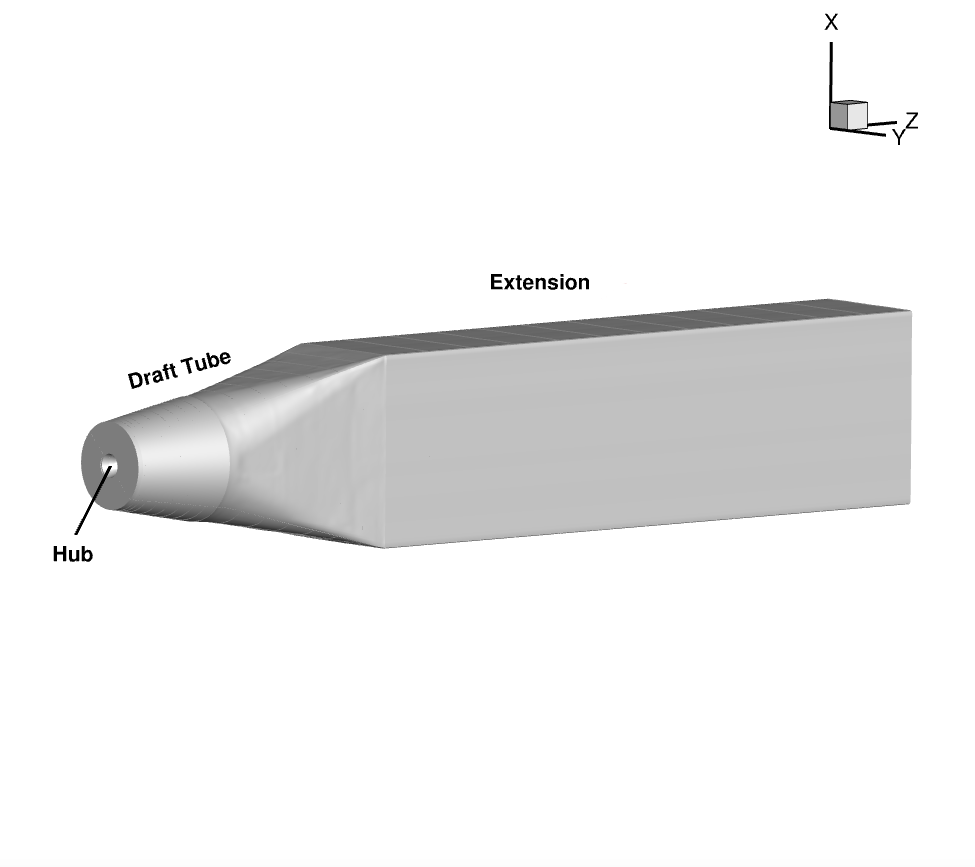
\includegraphics[clip=true, trim= 1.75cm 6.5cm 1.75cm 0.0cm,width=0.99\linewidth]{./figures/bulbt/geometry}                            
     \caption{Geometry of the grid.}
     \label{grid}
\end{figure}
%%%%%%%%%%%%%%%%%%%%%%%%%%%%%%%%%%%%%%%%%%%%%%%%%%%%%%%%%%%

The numerical simulations were performed on three consecutively refined grids, which consist of 3M, 14M and 50M cells respectively. The grid only consists of the hub, the draft tube and an extension as shown in Fig.~\ref{grid}. No-slip boundary condition is applied to all solid walls on the rotating hub and the stationary draft tube, while slip boundary condition is imposed on the solid walls of the extension. The inlet profile is extracted from a numerical simulation conducted with the complete turbine. At the outlet, a zero pressure boundary condition is imposed. The numerical simulations were performed with the baseline MUSCL scheme, the original and extended eddy-preserving limiter scheme. The dissipation of all three schemes were scaled down with a factor of $\alpha=0.375$ in computing the convective flux,
\begin{align} 
\mathbf{F}_{i+\frac{1}{2}} =\frac{1}{2}( \mathbf{F}(\mathbf{W}_{i+\frac{1}{2}}^{L})+\mathbf{F}(\mathbf{W}_{i+\frac{1}{2}}^{R})-\alpha \mathbf{P}^{-1} \lambda (\mathbf{W}_{i+\frac{1}{2}}^{R}-\mathbf{W}_{i+\frac{1}{2}}^{L})),
\label{rusanov}
\end{align}
where $\lambda$ is the spectral radius of the preconditioned Jacobian. The numerical results computed by the three schemes are denoted by ``MUSCL'', ``EDDY'', and ``EDDY-P'' respectively.
%%%%%%%%%%%%%%%%%%%%%%%%%%%%%%%%%%%%%%%%%%%%%%%%%%%%%%%%%%%
%%%%%%%%%%%%%%%%%%%%%%%%%%%%%%%%%%%%%%%%%%%%%%%%%%%%%%%%%%%
\begin{figure}[t]  
\centering      
     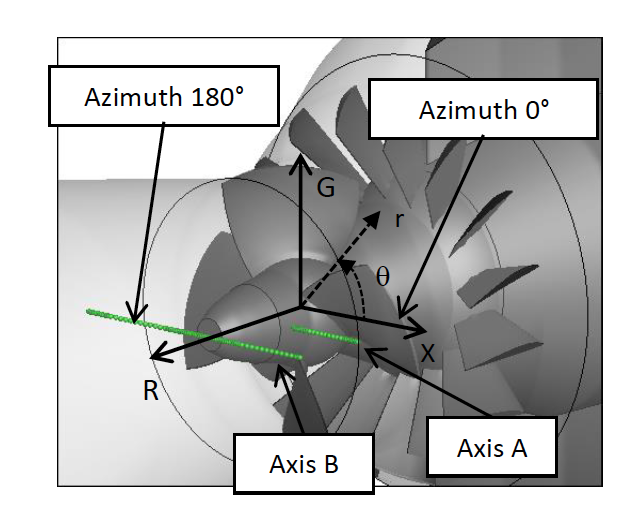
\includegraphics[clip=true, trim= 0.0cm 0.0cm 0.0cm 1.0cm,width=0.99\linewidth]{./figures/bulbt/Location4B}                  
     \caption{Location of 4BY0 \cite{vuillemard2014experimental}.}
     \label{plane4BY0}
\end{figure}
%%%%%%%%%%%%%%%%%%%%%%%%%%%%%%%%%%%%%%%%%%%%%%%%%%%%%%%%%%%

In the experiment, the axial and circumferential velocity profiles were measured by the Laser Doppler Velocimetry (LDV) at 4BY0, which is the green line labeled as Axis B in Fig.~\ref{plane4BY0}. As shown in Fig.~\ref{w} and Fig.~\ref{v}, in general, the agreement against the experimental data improves as the grid is refined. On each grid, the velocity profiles computed by all schemes are almost identical. However, zoom-in views of the velocity profiles show some differences in the central region. As shown in Fig.~\ref{zw}, in the experiment, there is a backflow region in the centre of the axial velocity profile. The MUSCL scheme shows poor predictions of the backflow region on all grids, while the EDDY and EDDY-P schemes can resolve the backflow region, and the predictions improve towards the experimental data as grid was refined. As for the experimental circumferential velocity, it first accelerates from the centre point in the direction of the runner rotation gently to a local maximum, which represents a forced vortex induced by the rotating hub. It then decelerates to zero, where the flow rotational direction is reversed. The circumferential velocity then subsequently accelerates in the reversed direction to a local maximum at approximately $x=\pm 0.023$ and then decelerates, which forms a shear flow here. In Fig.~\ref{zv}, all schemes do not predict the circumferential velocity very well in the central region on the 3M grid, but on the 14M and 50M grids, the EDDY and EDDY-P schemes outperform the MUSCL scheme significantly in predicting the locations as well as the magnitudes of the local maximums. 
%%%%%%%%%%%%%%%%%%%%%%%%%%%%%%%%%%%%%%%%%%%%%%%%%%%%%%%%%%%
%%%%%%%%%%%%%%%%%%%%%%%%%%%%%%%%%%%%%%%%%%%%%%%%%%%%%%%%%%%

The results for the turbulent kinetic energy (TKE) are plotted in Fig.~\ref{tke} and Fig.~\ref{ztke}. There are two peaks in the experiment, which corresponds to the shear flows at approximately $x=\pm 0.023$. Overall, the TKE profiles were underpredicted by all schemes in most of the region. Incorrect TKE peaks appear in the central region, which are mainly due to the deviation of the computed velocity profiles. As the grid was refined, the incorrect TKE peak at the central core reduces while the two side peaks edge upwards, showing a clear improving trend towards the experimental data. On each grid, compared to the MUSCL scheme, the EDDY and EDDY-P schemes predict slightly higher values at the two side peaks and lower values in the central core region, which leads to better agreement against the experimental data. 
%%%%%%%%%%%%%%%%%%%%%%%%%%%%%%%%%%%%%%%%%%%%%%%%%%%%%%%%%%%
%%%%%%%%%%%%%%%%%%%%%%%%%%%%%%%%%%%%%%%%%%%%%%%%%%%%%%%%%%%

The pressure profiles at 4BY0 are compared in Fig.~\ref{p}. The numerical result computed by the EDDY-P scheme on the 50M grid is employed as a reference, due to the lack of an experimental distribution of pressure across the cross-section of the draft tube, and denoted by ``EDDY-P-50M''. The EDDY-P scheme was used as the reference for two reasons; first, as the grid is refined, all schemes tend towards the results of the EDDY-P scheme on the 50M grid; and second, the EDDY-P pressure distribution seems more invariant to the grid refinement. The relative $L^{2}$ norms of difference against ``EDDY-P-50M'' for all schemes on all grids are shown in Table. \ref{table2}. On the 3M grid, due to the mispredicted gradients of the circumferencial velocity near the central region, all three schemes produce incorrect peaks in the pressure profile. On the 14M grid, the incorrect peaks of EDDY and EDDY-P are almost removed, and the prediction by the MUSCL is also improved. Moreover, compared to the prediction of EDDY, the prediction of EDDY-P is closer to the reference profile EDDY-P-50M, which shows that the dissipation of the scheme is further reduced. On the 50M grid, the peak for MUSCL continues to diminish, and the predictions of EDDY and EDDY-P almost equivalent. In summary, the EDDY and EDDY-P schemes produced better pressure profiles than the MUSCL scheme, and the EDDY-P is less dissipative than EDDY as expected. 
%%%%%%%%%%%%%%%%%%%%%%%%%%%%%%%%%%%%%%%%%%%%%%%%%%%%%%%%%%%

The profiles of the vorticity magnitude at 4BY0 are plotted in Fig.~\ref{vo}. Due to lack of an experimental radial velocity profile, the experimental vorticity magnitude was computed with the assumption that the flow is uniform in the circumferential direction. Three peaks are found in the experimental profile. The central peak represents the forced vortex induced by the rotating hub, while the two side peaks represent the shear flows at approximately $x=\pm 0.023$, where the circumferential velocity accelerates to a local maximum and then decelerates. On the 3M grid, all schemes overpredict the vorticity magnitude in the centre, due to the mispredicted gradients of circumferential velocity, as shown in Fig.~\ref{v}(a). On the 14M and 50M grids, the MUSCL scheme still overpredicts the peak in the centre, while the EDDY and EDDY-P schemes only slightly underpredict the peak. It is also notable that as the grid was refined, the two side peaks due to the shear flows were captured.

%%%%%%%%%%%%%%%%%%%%%%%%%%%%%%%%%%%%%%%%%%%%%%%%%%%%%%%%%%%
The comparisons demonstrate that the original and extended eddy-preserving limiter schemes are capable of producing better predictions for velocity, TKE and pressure profiles than the baseline MUSCL scheme, and the extended eddy-preserving limiter scheme has a lower dissipation for the prediction of pressure than the original eddy-preserving limiter scheme.
%%%%%%%%%%%%%%%%%%%%%%%%%%%%%%%%%%%%%%%%%%%%%%%%%%%%%%%%%%%%%%%%
%%%%%%%%%%%%%%%%%%%%%%%%%%%%%%%%%%%%%%%%%%%%%%%%%%%%%%%%%%%%%%%%
%%%%%%%%%%%%%%%%%%%%%%%%%%%%%%%%%%%%%%%%%%%%%%%%%%%%%%%%%%%%%%%%
%%%%%%%%%%%%%%%%%%%%%%%%%%%%%%%%%%%%%%%%%%%%%%%%%%%%%%%%%%%%%%%%
%%%%%%%%%%%%%%%%%%%%%%%%%%%%%%%%%%%%%%%%%%%%%%%%%%%%%%%%%%%%%%%%
\begin{figure}[t]  
\centering
%\begin{minipage}{.99\textwidth}
\centering
     \subfigure[]{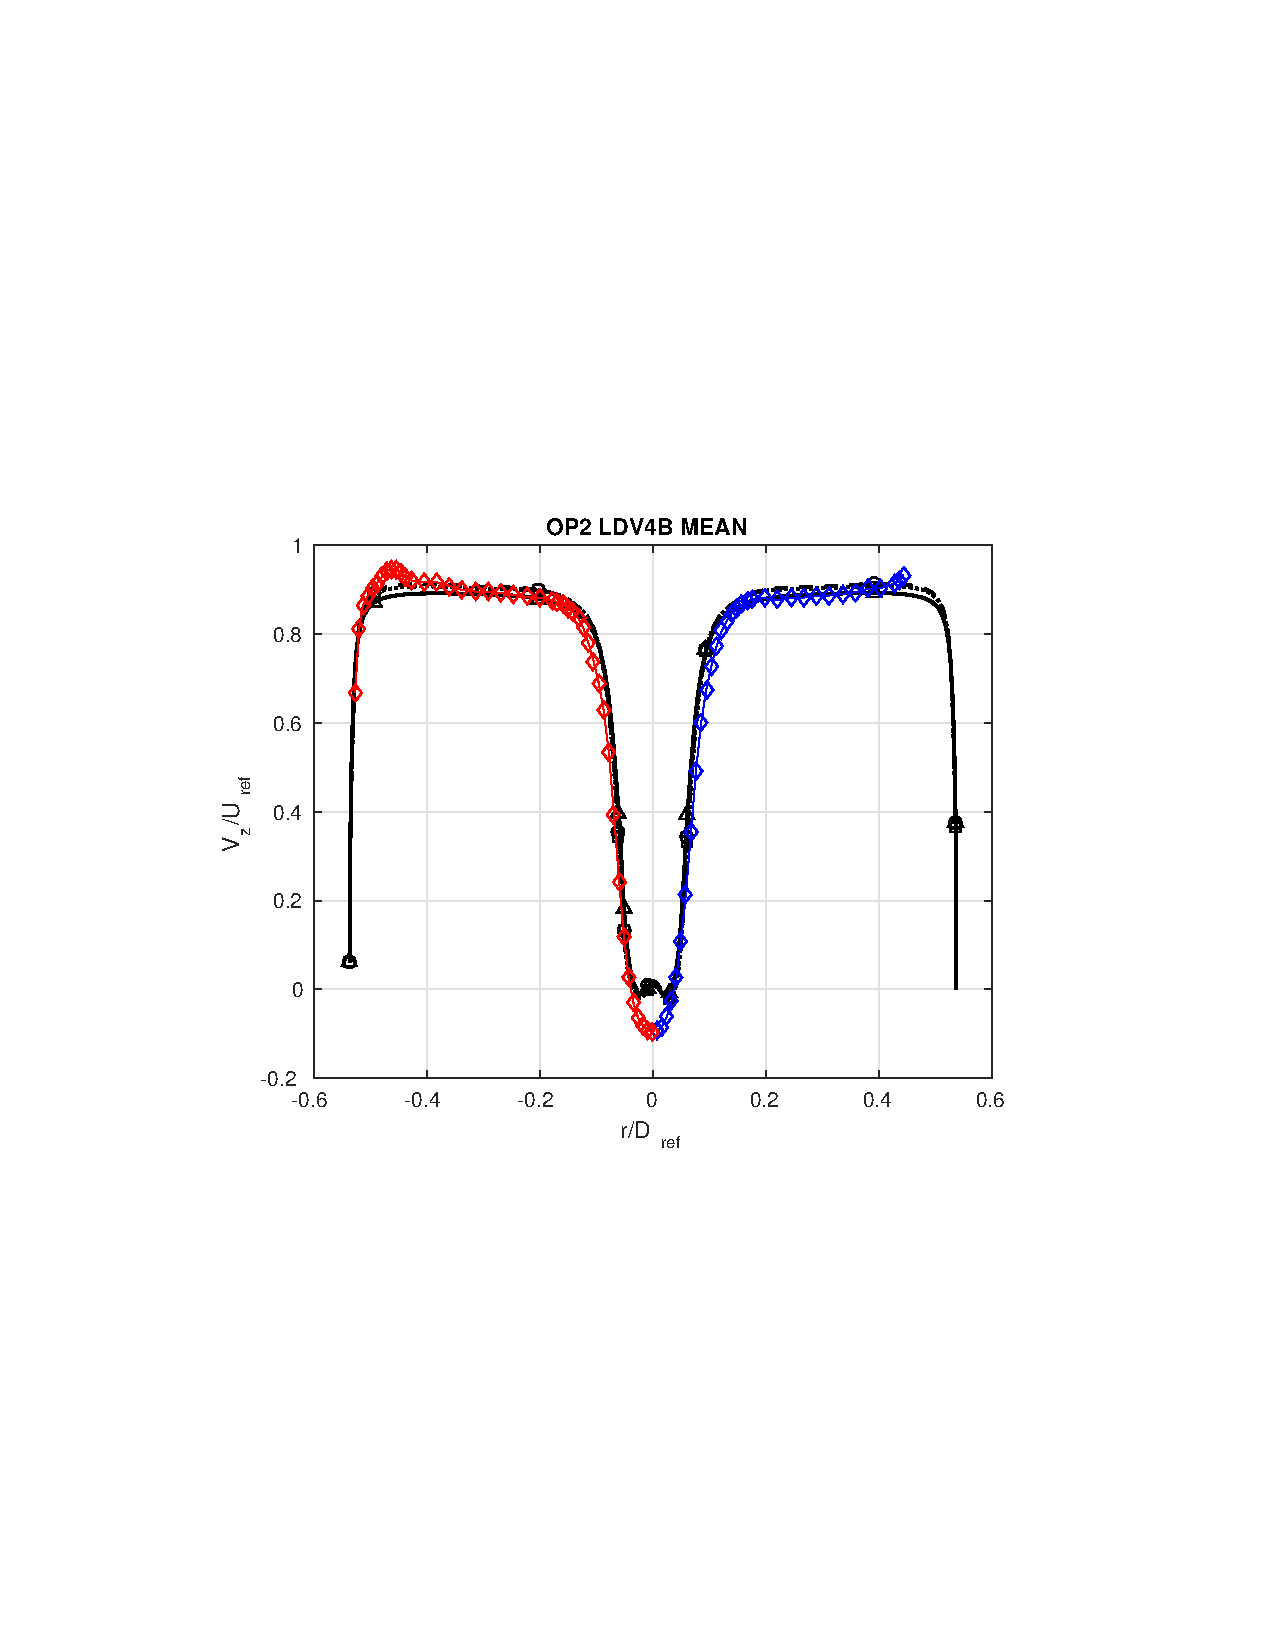
\includegraphics[clip=true, trim= 3.0cm 8.0cm 4.0cm 8.0cm,width=0.98\linewidth]{./figures/bulbt/4BY0/3m/multi_plan4BY0_BulbT_op2_uncert_X_w}} \\             
     \subfigure[]{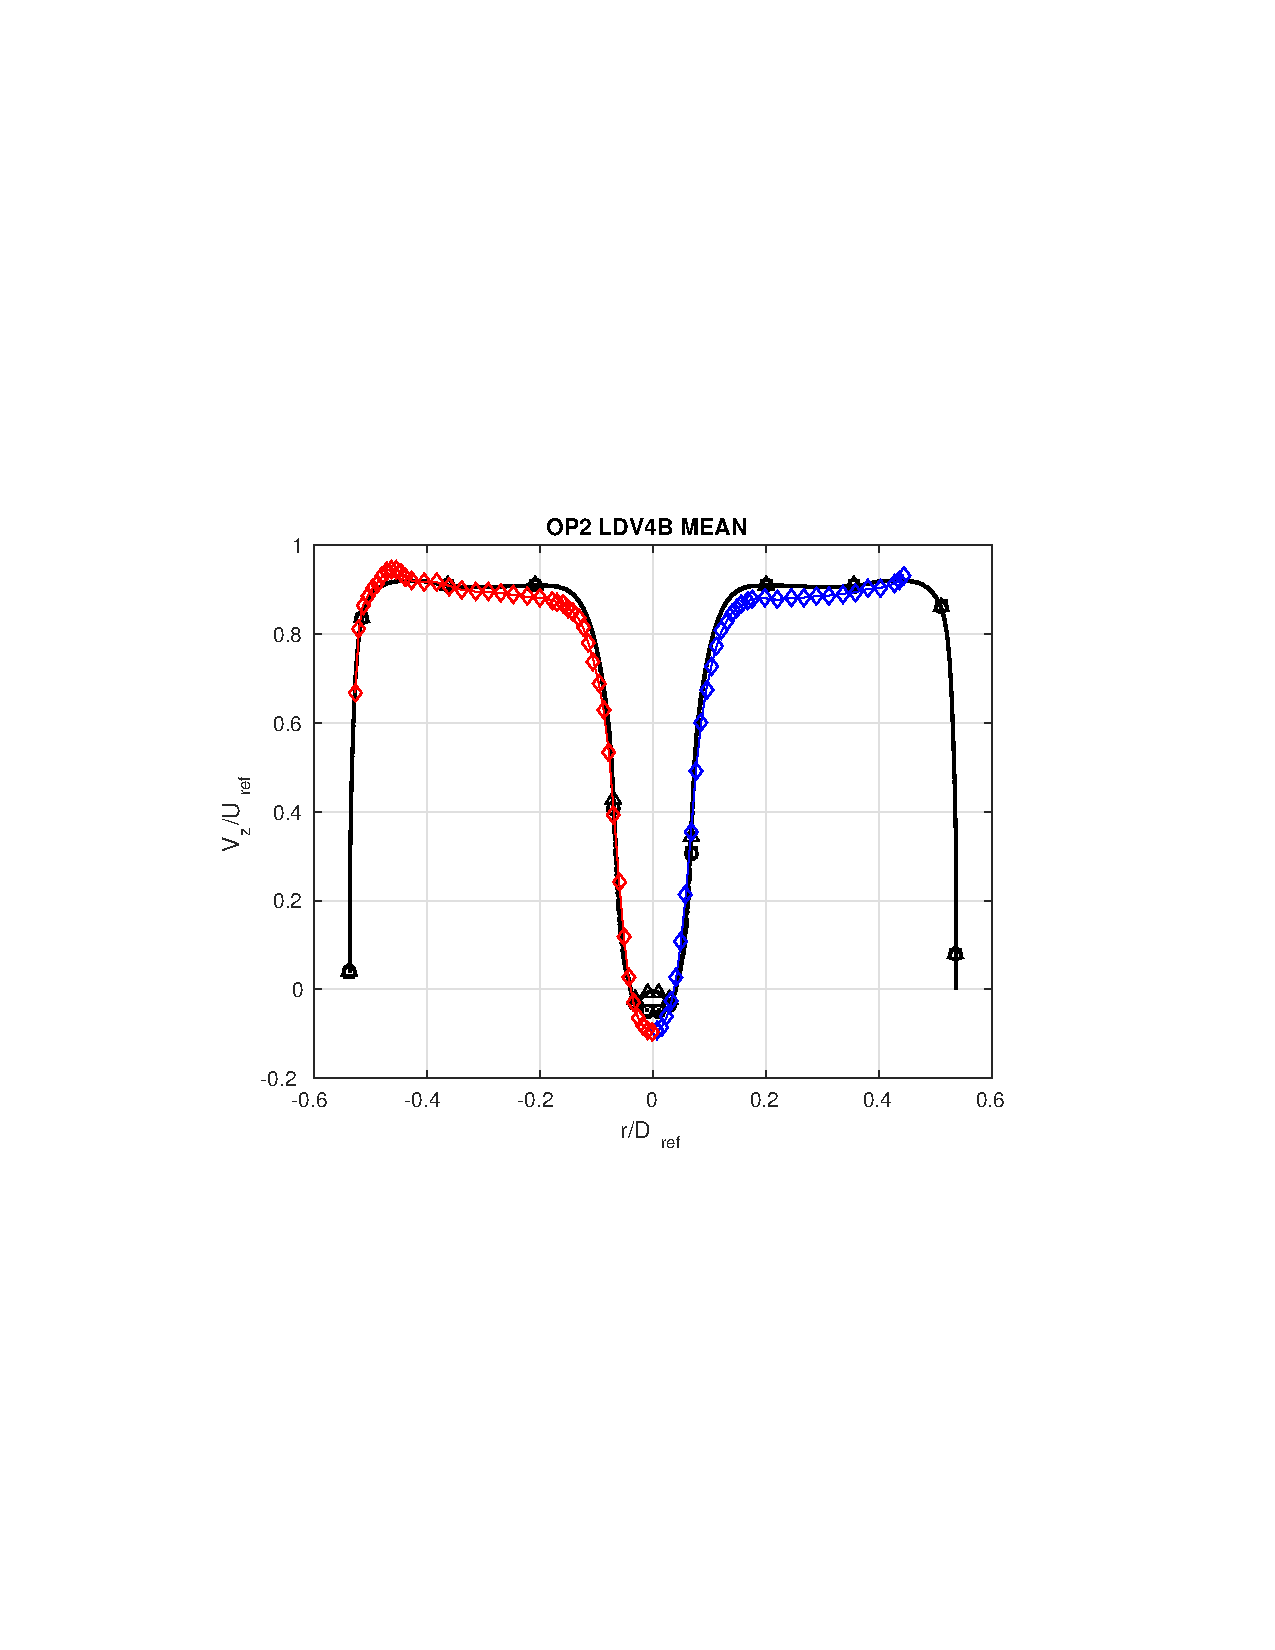
\includegraphics[clip=true, trim= 3.0cm 8.0cm 4.0cm 8.0cm,width=0.98\linewidth]{./figures/bulbt/4BY0/14m/multi_plan4BY0_BulbT_op2_uncert_X_w}} \\
     \subfigure[]{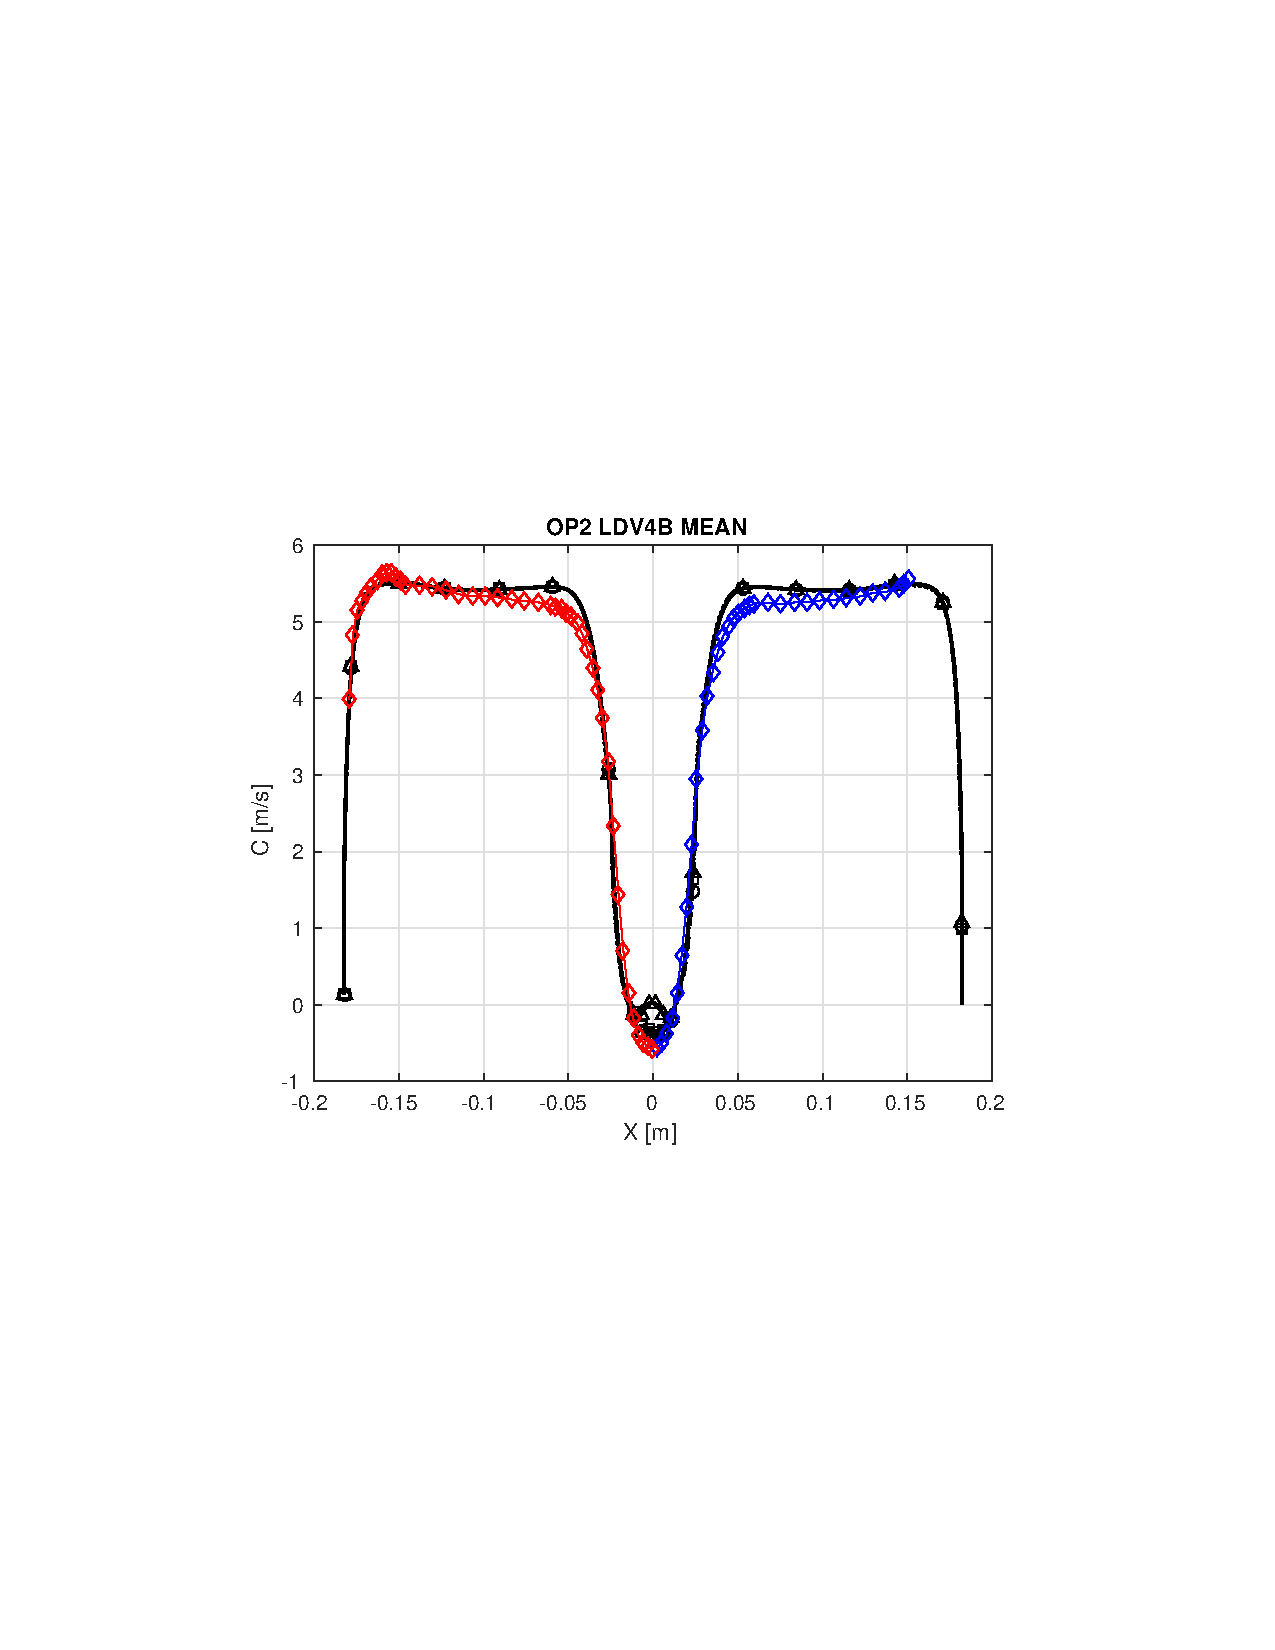
\includegraphics[clip=true, trim= 3.0cm 8.0cm 4.0cm 8.0cm,width=0.98\linewidth]{./figures/bulbt/4BY0/50m/multi_plan4BY0_BulbT_op2_uncert_X_w}}       
     \caption{Axial velocity profiles at plane 4BY0 on (a)3M (b)14M (c)50M grid. (MUSCL: \mline; EDDY: \eline; EDDY-P: \epline; EXP Cz Az0: \bluediam; EXP Cz Az180: \reddiam.)}
     \label{w} 
%     \end{minipage}          
\end{figure}
%%%%%%%%%%%%%%%%%%%%%%%%%%%%%%%%%%%%%%%%%%%%%%%%%%%%%%%%%%%%%%%%
\begin{figure}[t]  
\centering
%\begin{minipage}{.99\textwidth}
\centering
     \subfigure[]{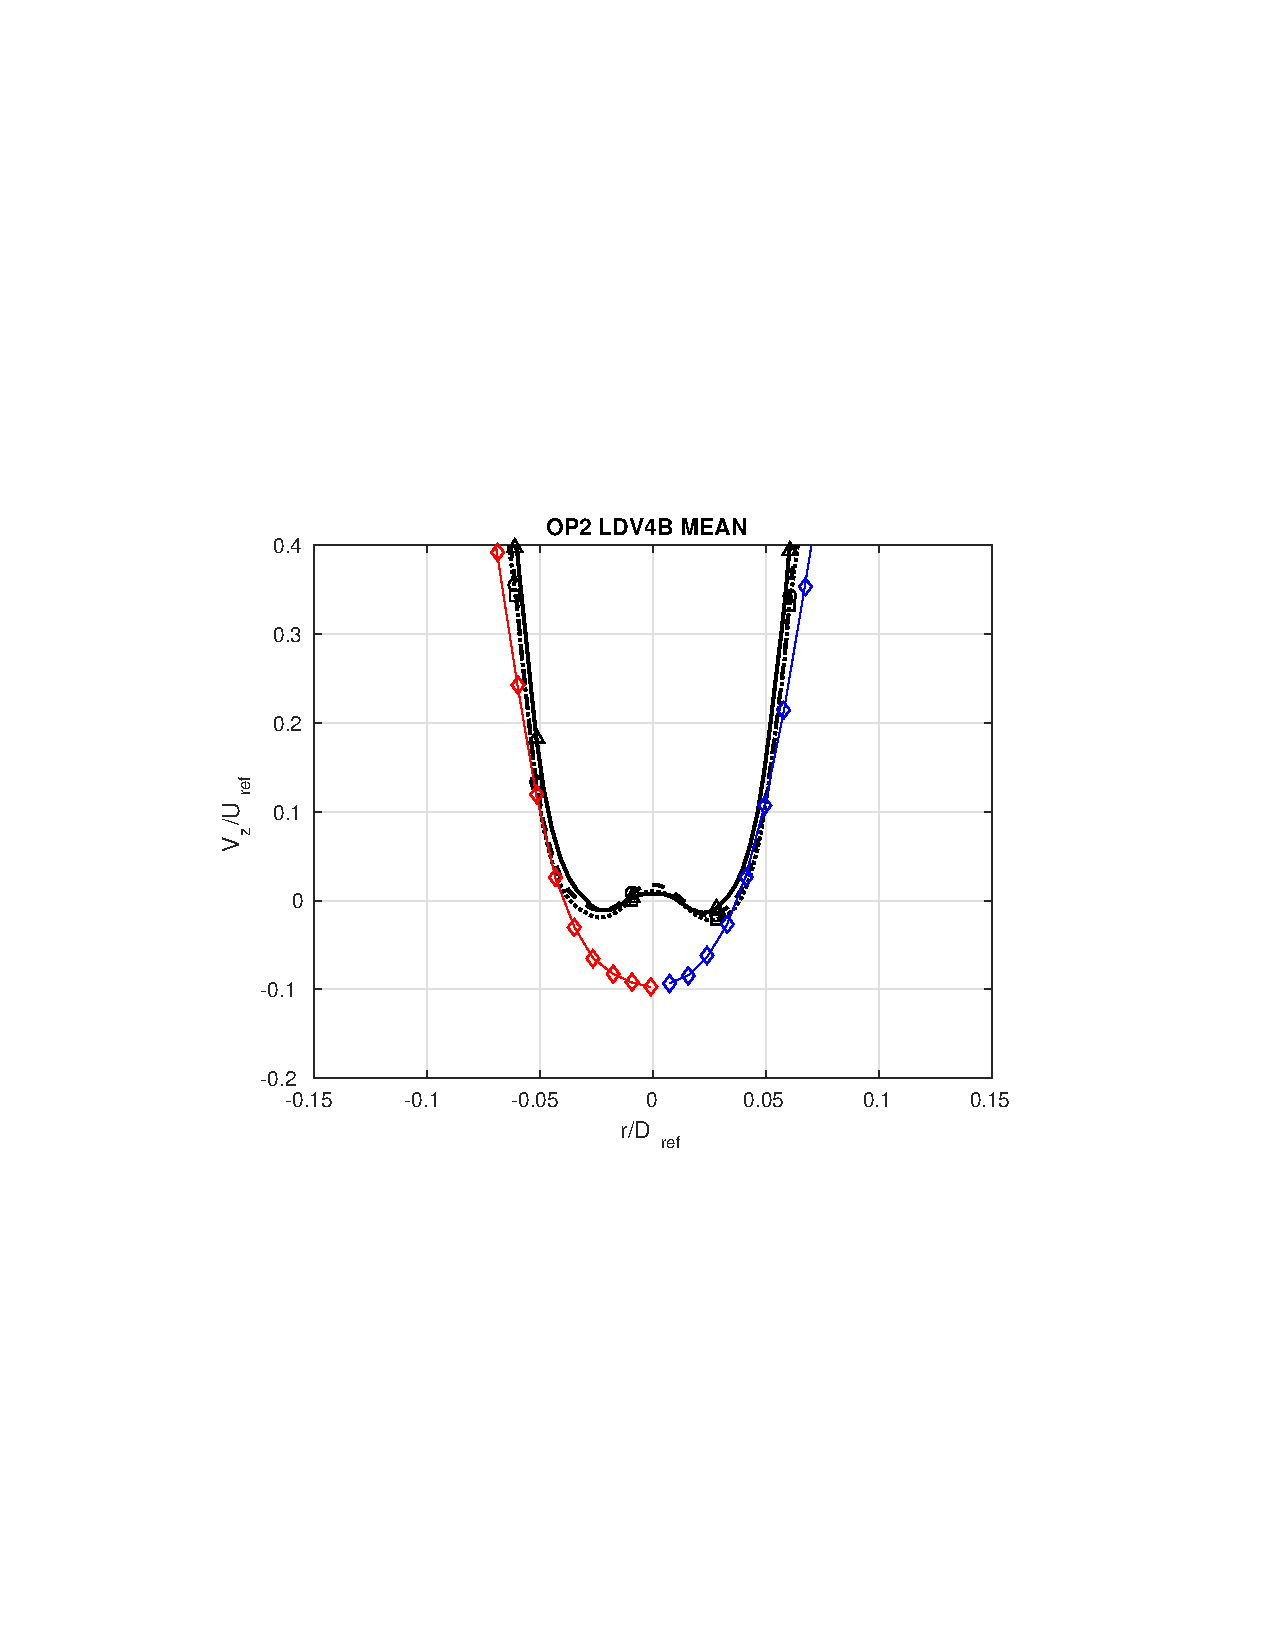
\includegraphics[clip=true, trim= 3.0cm 8.0cm 4.0cm 8.0cm,width=0.98\linewidth]{./figures/bulbt/4BY0/3m/zoom_multi_plan4BY0_BulbT_op2_uncert_X_w}} \\             
     \subfigure[]{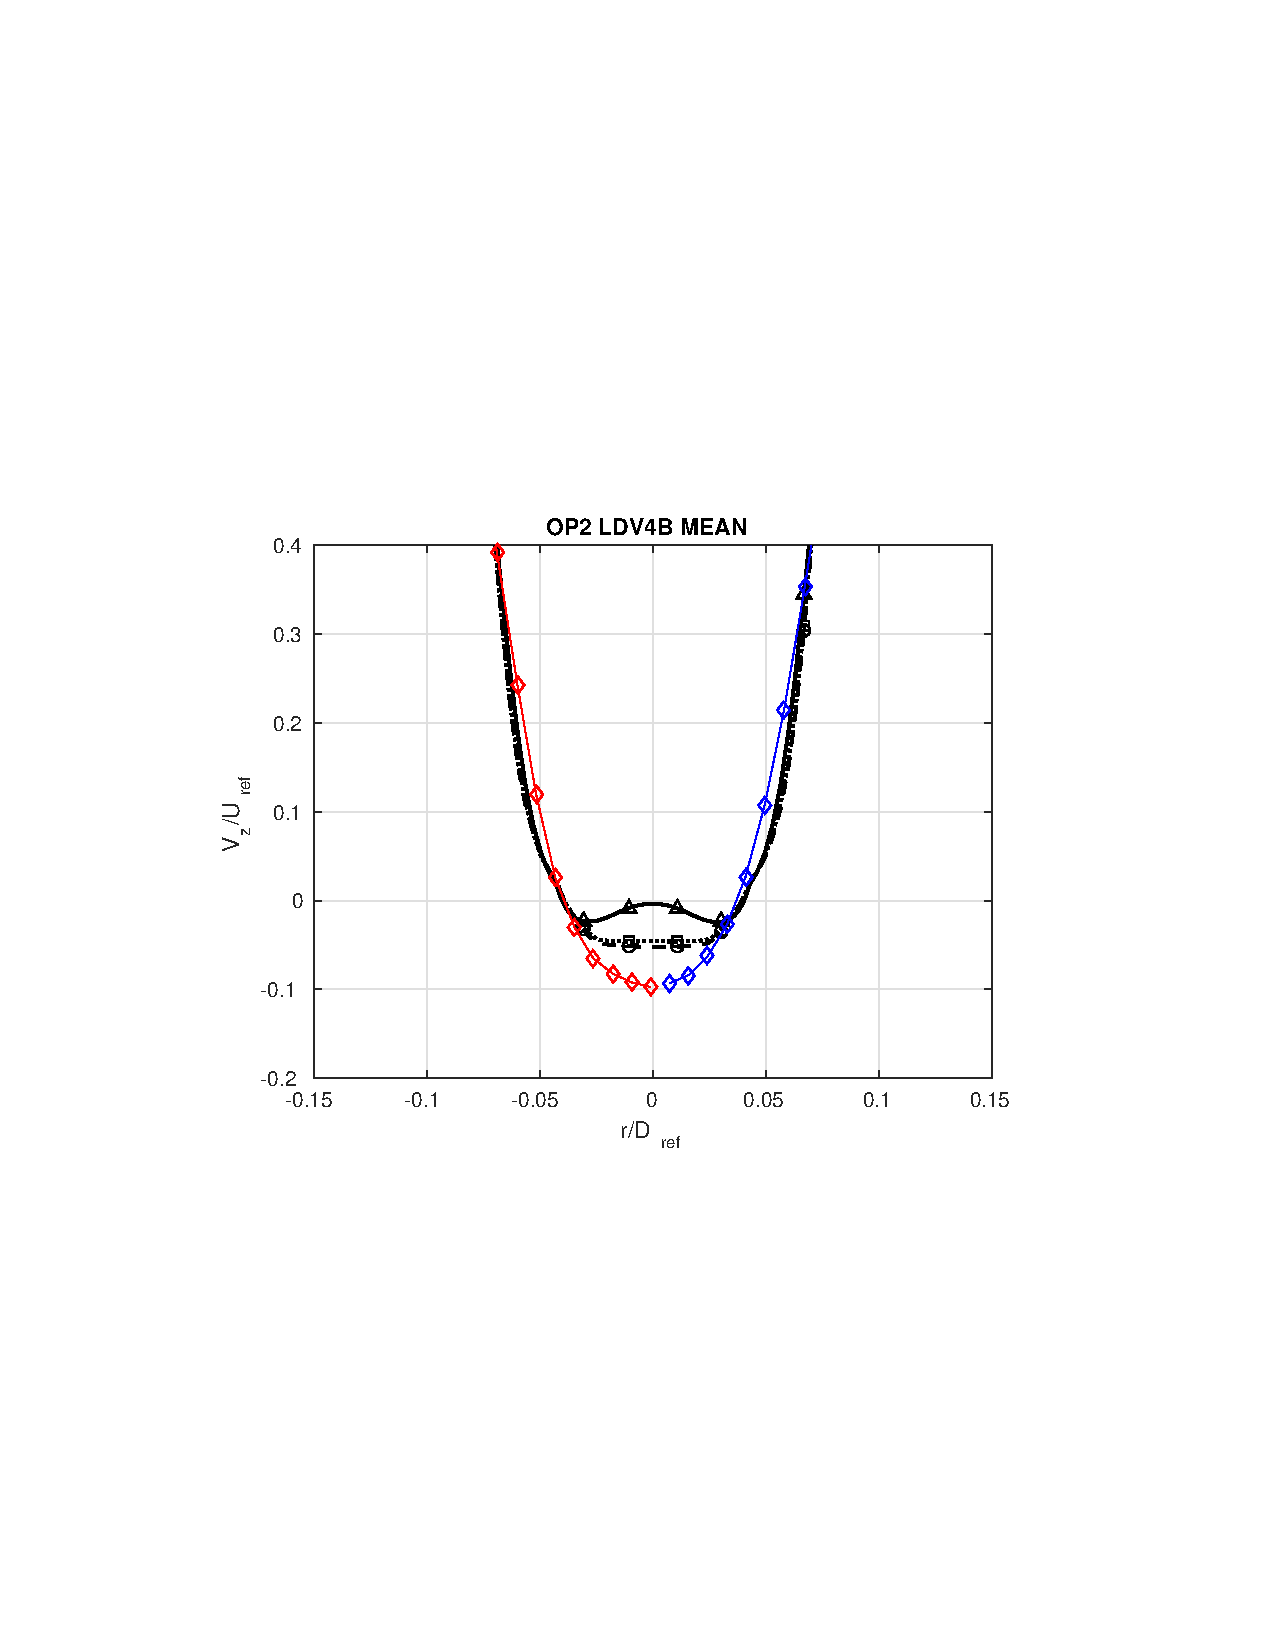
\includegraphics[clip=true, trim= 3.0cm 8.0cm 4.0cm 8.0cm,width=0.98\linewidth]{./figures/bulbt/4BY0/14m/zoom_multi_plan4BY0_BulbT_op2_uncert_X_w}} \\
     \subfigure[]{\includegraphics[clip=true, trim= 3.0cm 8.0cm 4.0cm 8.0cm,width=0.98\linewidth]{./figures/bulbt/4BY0/50m/zoom_multi_plan4BY0_BulbT_op2_uncert_X_w}}     
     \caption{Zoom-in view of axial velocity profiles at plane 4BY0 on (a)3M (b)14M (c)50M grid. (MUSCL: \mline; EDDY: \eline; EDDY-P: \epline; EXP Cz Az0: \bluediam; EXP Cz Az180: \reddiam.)}
     \label{zw} 
%     \end{minipage}          
\end{figure}
%%%%%%%%%%%%%%%%%%%%%%%%%%%%%%%%%%%%%%%%%%%%%%%%%%%%%%%%%%%%%%%%
%%%%%%%%%%%%%%%%%%%%%%%%%%%%%%%%%%%%%%%%%%%%%%%%%%%%%%%%%%%%%%%%
\begin{figure}[t]  
\centering
%\begin{minipage}{.99\textwidth}
\centering
     \subfigure[]{\includegraphics[clip=true, trim= 3.0cm 8.0cm 4.0cm 8.0cm,width=0.98\linewidth]{./figures/bulbt/4BY0/3m/multi_plan4BY0_BulbT_op2_uncert_X_v}} \\             
     \subfigure[]{\includegraphics[clip=true, trim= 3.0cm 8.0cm 4.0cm 8.0cm,width=0.98\linewidth]{./figures/bulbt/4BY0/14m/multi_plan4BY0_BulbT_op2_uncert_X_v}} \\
     \subfigure[]{\includegraphics[clip=true, trim= 3.0cm 8.0cm 4.0cm 8.0cm,width=0.98\linewidth]{./figures/bulbt/4BY0/50m/multi_plan4BY0_BulbT_op2_uncert_X_v}}     
     \caption{Circumferential velocity profiles at plane 4BY0 on (a)3M (b)14M (c)50M grid. (MUSCL: \mline; EDDY: \eline; EDDY-P: \epline; EXP Cy Az0: \bluecrx; EXP Cy Az180: \redcrx.)}
     \label{v} 
%     \end{minipage}          
\end{figure}
%%%%%%%%%%%%%%%%%%%%%%%%%%%%%%%%%%%%%%%%%%%%%%%%%%%%%%%%%%%%%%%%
\begin{figure}[t]  
\centering
%\begin{minipage}{.99\textwidth}
\centering
     \subfigure[]{\includegraphics[clip=true, trim= 3.0cm 8.0cm 4.0cm 8.0cm,width=0.98\linewidth]{./figures/bulbt/4BY0/3m/zoom_multi_plan4BY0_BulbT_op2_uncert_X_v}} \\             
     \subfigure[]{\includegraphics[clip=true, trim= 3.0cm 8.0cm 4.0cm 8.0cm,width=0.98\linewidth]{./figures/bulbt/4BY0/14m/zoom_multi_plan4BY0_BulbT_op2_uncert_X_v}} \\
     \subfigure[]{\includegraphics[clip=true, trim= 3.0cm 8.0cm 4.0cm 8.0cm,width=0.98\linewidth]{./figures/bulbt/4BY0/50m/zoom_multi_plan4BY0_BulbT_op2_uncert_X_v}}        
     \caption{Zoom-in view of circumferential velocity profiles at plane 4BY0 on (a)3M (b)14M (c)50M grid. (MUSCL: \mline; EDDY: \eline; EDDY-P: \epline; EXP Cy Az0: \bluecrx; EXP Cy Az180: \redcrx.)}
     \label{zv} 
%     \end{minipage}          
\end{figure}
%%%%%%%%%%%%%%%%%%%%%%%%%%%%%%%%%%%%%%%%%%%%%%%%%%%%%%%%%%%%%%%%
%%%%%%%%%%%%%%%%%%%%%%%%%%%%%%%%%%%%%%%%%%%%%%%%%%%%%%%%%%%%%%%%
\begin{figure}[t]  
\centering
%\begin{minipage}{.99\textwidth}
\centering
     \subfigure[]{\includegraphics[clip=true, trim= 3.0cm 8.0cm 4.0cm 8.0cm,width=0.98\linewidth]{./figures/bulbt/4BY0/3m/multi_plan4BY0_BulbT_op2_Tke_X}} \\             
     \subfigure[]{\includegraphics[clip=true, trim= 3.0cm 8.0cm 4.0cm 8.0cm,width=0.98\linewidth]{./figures/bulbt/4BY0/14m/multi_plan4BY0_BulbT_op2_Tke_X}} \\
     \subfigure[]{\includegraphics[clip=true, trim= 3.0cm 8.0cm 4.0cm 8.0cm,width=0.98\linewidth]{./figures/bulbt/4BY0/50m/multi_plan4BY0_BulbT_op2_Tke_X}}        
     \caption{TKE profiles at plane 4BY0 on (a)3M (b)14M (c)50M grid.  (MUSCL: \mline; EDDY: \eline; EDDY-P: \epline; EXP TKE Az0: \bluediam; EXP TKE Az180: \reddiam.)}
     \label{tke} 
%     \end{minipage}          
\end{figure}
%%%%%%%%%%%%%%%%%%%%%%%%%%%%%%%%%%%%%%%%%%%%%%%%%%%%%%%%%%%%%%%%
\begin{figure}[t]  
\centering
%\begin{minipage}{.99\textwidth}
\centering
     \subfigure[]{\includegraphics[clip=true, trim= 3.0cm 8.0cm 4.0cm 8.0cm,width=0.98\linewidth]{./figures/bulbt/4BY0/3m/zoom_multi_plan4BY0_BulbT_op2_Tke_X}} \\             
     \subfigure[]{\includegraphics[clip=true, trim= 3.0cm 8.0cm 4.0cm 8.0cm,width=0.98\linewidth]{./figures/bulbt/4BY0/14m/zoom_multi_plan4BY0_BulbT_op2_Tke_X}} \\
     \subfigure[]{\includegraphics[clip=true, trim= 3.0cm 8.0cm 4.0cm 8.0cm,width=0.98\linewidth]{./figures/bulbt/4BY0/50m/zoom_multi_plan4BY0_BulbT_op2_Tke_X}}       
     \caption{Zoom-in view of TKE profiles at plane 4BY0 on (a)3M (b)14M (c)50M grid. (MUSCL: \mline; EDDY: \eline; EDDY-P: \epline; EXP TKE Az0: \bluediam; EXP TKE Az180: \reddiam.)}
     \label{ztke} 
%     \end{minipage}          
\end{figure}
%%%%%%%%%%%%%%%%%%%%%%%%%%%%%%%%%%%%%%%%%%%%%%%%%%%%%%%%%%%%%%%%
%%%%%%%%%%%%%%%%%%%%%%%%%%%%%%%%%%%%%%%%%%%%%%%%%%%%%%%%%%%%%%%%
%%%%%%%%%%%%%%%%%%%%%%%%%%%%%%%%%%%%%%%%%%%%%%%%%%%%%%%%%%%%%%%%
%%%%%%%%%%%%%%%%%%%%%%%%%%%%%%%%%%%%%%%%%%%%%%%%%%%%%%%%%%%%%%%%
\begin{figure}[t]  
\centering
%\begin{minipage}{.99\textwidth}
\centering
     \subfigure[]{\includegraphics[clip=true, trim= 1.25cm 1.25cm 3.25cm 3.25cm,width=0.98\linewidth]{./figures/bulbt/P/3m}} \\             
     \subfigure[]{\includegraphics[clip=true, trim= 1.25cm 1.25cm 3.25cm 3.25cm,width=0.98\linewidth]{./figures/bulbt/P/14m}} \\
     \subfigure[]{\includegraphics[clip=true, trim= 1.25cm 1.25cm 3.25cm 3.25cm,width=0.98\linewidth]{./figures/bulbt/P/50m}}     
     \caption{Pressure profiles at plane 4BY0 on (a)3M (b)14M (c)50M grid.}
     \label{p}     
%     \end{minipage}          
\end{figure}
%%%%%%%%%%%%%%%%%%%%%%%%%%%%%%%%%%%%%%%%%%%%%%%%%%%%%%%%%%%%%%%%
%%%%%%%%%%%%%%%%%%%%%%%%%%%%%%%%%%%%%%%%%%%%%%%%%%%%%%%%%%%%%%%%
%%%%%%%%%%%%%%%%%%%%%%%%%%%%%%%%%%%%%%%%%%%%%%%%%%%%%%%%%%%%%%%%
%%%%%%%%%%%%%%%%%%%%%%%%%%%%%%%%%%%%%%%%%%%%%%%%%%%%%%%%%%%%%%%%
\begin{figure}[t]  
\centering
%\begin{minipage}{.99\textwidth}
\centering
     \subfigure[]{\includegraphics[clip=true, trim= 1.25cm 1.25cm 3.25cm 3.25cm,width=0.98\linewidth]{./figures/bulbt/4by0vo/3m}} \\            
     \subfigure[]{\includegraphics[clip=true, trim= 1.25cm 1.25cm 3.25cm 3.25cm,width=0.98\linewidth]{./figures/bulbt/4by0vo/14m}} \\
     \subfigure[]{\includegraphics[clip=true, trim= 1.25cm 1.25cm 3.25cm 3.25cm,width=0.98\linewidth]{./figures/bulbt/4by0vo/50m}}        
     \caption{Vorticity magnitude at plane 4BY0 on (a)3M (b)14M (c)50M grid. (MUSCL: \mline; EDDY: \eline; EDDY-P: \epline; EXP: \exact.)}
     \label{vo} 
%     \end{minipage}          
\end{figure}
%%%%%%%%%%%%%%%%%%%%%%%%%%%%%%%%%%%%%%%%%%%%%%%%%%%%%%%%%%%%%%%%
%\FloatBarrier
\begin{table}[t]
\caption{Relative $L^{2}$ norms of difference for pressure profiles.}
\begin{center}
\label{table2}
\begin{tabular}{c l l l}
\hline
Scheme & 3M     & 14M    & 50M    \\ 
\hline
MUSCL  & 0.2872 & 0.0953 & 0.0458 \\ 
EDDY   & 0.2105 & 0.0776 & 0.0166 \\ 
EDDY-P & 0.0750 & 0.0743 & 0.0000 \\
\hline 
\end{tabular}
\end{center}
\end{table}
%%%%%%%%%%%%%%%%%%%%%%%%%%%%%%%%%%%%%%%%%%%%%%%%%%%%%%%%%%%%%%%%












































%%%%%%%%%%%%%%%%%%%%%%%%%%%%%%%%%%%%%%%%%%%%%%%%%%%%%%%%%%%%%%%%%%
%%\begin{figure}[!htb]  
%%\centering
%%\begin{minipage}{.99\textwidth}
%%\centering
%%     \subfigure[]{\includegraphics[clip=true, trim= 3.0cm 8.0cm 4.0cm 8.0cm,width=0.98\linewidth]{./figures/bulbt/4BY0/3m/multi_plan4BY0_BulbT_op2_uncert_X}} \\             
%%     \subfigure[]{\includegraphics[clip=true, trim= 3.0cm 8.0cm 4.0cm 8.0cm,width=0.98\linewidth]{./figures/bulbt/4BY0/14m/multi_plan4BY0_BulbT_op2_uncert_X}} \\
%%     \subfigure[]{\includegraphics[clip=true, trim= 3.0cm 8.0cm 4.0cm 8.0cm,width=0.98\linewidth]{./figures/bulbt/4BY0/50m/multi_plan4BY0_BulbT_op2_uncert_X}}  \\       
%%     \caption{Velocity profiles at plane 4BY0 on (a)3M (b)14M (c)50M grid. (MUSCL: \mline; EDDY: \eline; EDDY-P: \epline; EXP Cz Az0: \bluediam; EXP Cz Az180: \reddiam; EXP Cy Az0: \bluecrx; EXP Cy Az180: \redcrx.)}
%%     \label{u} 
%%     \end{minipage}          
%%\end{figure}
%%%%%%%%%%%%%%%%%%%%%%%%%%%%%%%%%%%%%%%%%%%%%%%%%%%%%%%%%%%%%%%%%%
%%\begin{figure}[!htb]  
%%\centering
%%\begin{minipage}{.99\textwidth}
%%\centering
%%     \subfigure[]{\includegraphics[clip=true, trim= 3.0cm 8.0cm 4.0cm 8.0cm,width=0.98\linewidth]{./figures/bulbt/4BY0/3m/zoom_multi_plan4BY0_BulbT_op2_uncert_X}} \\             
%%     \subfigure[]{\includegraphics[clip=true, trim= 3.0cm 8.0cm 4.0cm 8.0cm,width=0.98\linewidth]{./figures/bulbt/4BY0/14m/zoom_multi_plan4BY0_BulbT_op2_uncert_X}} \\
%%     \subfigure[]{\includegraphics[clip=true, trim= 3.0cm 8.0cm 4.0cm 8.0cm,width=0.98\linewidth]{./figures/bulbt/4BY0/50m/zoom_multi_plan4BY0_BulbT_op2_uncert_X}} \\        
%%     \caption{Zoom-in view of velocity profiles at plane 4BY0 on (a)3M (b)14M (c)50M grid. (MUSCL: \mline; EDDY: \eline; EDDY-P: \epline; EXP Cz Az0: \bluediam; EXP Cz Az180: \reddiam; EXP Cy Az0: \bluecrx; EXP Cy Az180: \redcrx.)}
%%     \label{zu} 
%%     \end{minipage}          
%%\end{figure}
%%%%%%%%%%%%%%%%%%%%%%%%%%%%%%%%%%%%%%%%%%%%%%%%%%%%%%%%%%%%%%%%%%
%%%%%%%%%%%%%%%%%%%%%%
%\begin{figure}[!htb]  
%\centering
%\begin{minipage}{.99\textwidth}
%     \subfigure[]{\includegraphics[clip=true, trim= 3.0cm 8.0cm 4.0cm 8.0cm,width=0.32\linewidth]{./figures/bulbt/4BY0/3m/multi_plan4BY0_BulbT_op2_uncert_X}}              
%     \subfigure[]{\includegraphics[clip=true, trim= 3.0cm 8.0cm 4.0cm 8.0cm,width=0.32\linewidth]{./figures/bulbt/4BY0/14m/multi_plan4BY0_BulbT_op2_uncert_X}} 
%     \subfigure[]{\includegraphics[clip=true, trim= 3.0cm 8.0cm 4.0cm 8.0cm,width=0.32\linewidth]{./figures/bulbt/4BY0/50m/multi_plan4BY0_BulbT_op2_uncert_X}}         
%     \caption{Velocity profiles at plane 4BY0 on (a)3M (b)14M (c)50M grid. (MUSCL: \mline; EDDY: \eline; EDDY-P: \epline; EXP Cz Az0: \bluediam; EXP Cz Az180: \reddiam; EXP Cy Az0: \bluecrx; EXP Cy Az180: \redcrx.)}
%     \label{u} 
%     \end{minipage}          
%\end{figure}
%%%%%%%%%%%%%%%%%%%%%%%%%%%%%%%%%%%%%%%%%%%%%%%%%%%%%%%%%%%%%%%%%
%\begin{figure}[!htb]  
%\centering
%\begin{minipage}{.99\textwidth}
%     \subfigure[]{\includegraphics[clip=true, trim= 3.0cm 8.0cm 4.0cm 8.0cm,width=0.32\linewidth]{./figures/bulbt/4BY0/3m/zoom_multi_plan4BY0_BulbT_op2_uncert_X}}              
%     \subfigure[]{\includegraphics[clip=true, trim= 3.0cm 8.0cm 4.0cm 8.0cm,width=0.32\linewidth]{./figures/bulbt/4BY0/14m/zoom_multi_plan4BY0_BulbT_op2_uncert_X}} 
%     \subfigure[]{\includegraphics[clip=true, trim= 3.0cm 8.0cm 4.0cm 8.0cm,width=0.32\linewidth]{./figures/bulbt/4BY0/50m/zoom_multi_plan4BY0_BulbT_op2_uncert_X}}         
%     \caption{Zoom-in view of velocity profiles at plane 4BY0 on (a)3M (b)14M (c)50M grid. (MUSCL: \mline; EDDY: \eline; EDDY-P: \epline; EXP Cz Az0: \bluediam; EXP Cz Az180: \reddiam; EXP Cy Az0: \bluecrx; EXP Cy Az180: \redcrx.)}
%     \label{zu} 
%     \end{minipage}          
%\end{figure}
%%%%%%%%%%%%%%%%%%%%%%%%%%%%%%%%%%%%%%%%%%%%%%%%%%%%%%%%%%%%%%%%%
%%%%%%%%%%%%%%%%%%%%%%%%%%%%%%%%%%%%%%%%%%%%%%%%%%%%%%%%%%%%%%%%%
%\begin{figure}[!htb]  
%\centering
%\begin{minipage}{.99\textwidth}
%     \subfigure[]{\includegraphics[clip=true, trim= 3.0cm 8.0cm 4.0cm 8.0cm,width=0.32\linewidth]{./figures/bulbt/4BY0/3m/multi_plan4BY0_BulbT_op2_Tke_X}}              
%     \subfigure[]{\includegraphics[clip=true, trim= 3.0cm 8.0cm 4.0cm 8.0cm,width=0.32\linewidth]{./figures/bulbt/4BY0/14m/multi_plan4BY0_BulbT_op2_Tke_X}} 
%     \subfigure[]{\includegraphics[clip=true, trim= 3.0cm 8.0cm 4.0cm 8.0cm,width=0.32\linewidth]{./figures/bulbt/4BY0/50m/multi_plan4BY0_BulbT_op2_Tke_X}}         
%     \caption{TKE profiles at plane 4BY0 on (a)3M (b)14M (c)50M grid.  (MUSCL: \mline; EDDY: \eline; EDDY-P: \epline; EXP TKE Az0: \bluediam; EXP TKE Az180: \reddiam.)}
%     \label{tke} 
%     \end{minipage}          
%\end{figure}
%%%%%%%%%%%%%%%%%%%%%%%%%%%%%%%%%%%%%%%%%%%%%%%%%%%%%%%%%%%%%%%%%
%\begin{figure}[!htb]  
%\centering
%\begin{minipage}{.99\textwidth}
%     \subfigure[]{\includegraphics[clip=true, trim= 3.0cm 8.0cm 4.0cm 8.0cm,width=0.32\linewidth]{./figures/bulbt/4BY0/3m/zoom_multi_plan4BY0_BulbT_op2_Tke_X}}              
%     \subfigure[]{\includegraphics[clip=true, trim= 3.0cm 8.0cm 4.0cm 8.0cm,width=0.32\linewidth]{./figures/bulbt/4BY0/14m/zoom_multi_plan4BY0_BulbT_op2_Tke_X}} 
%     \subfigure[]{\includegraphics[clip=true, trim= 3.0cm 8.0cm 4.0cm 8.0cm,width=0.32\linewidth]{./figures/bulbt/4BY0/50m/zoom_multi_plan4BY0_BulbT_op2_Tke_X}}         
%     \caption{Zoom-in view of TKE profiles at plane 4BY0 on (a)3M (b)14M (c)50M grid. (MUSCL: \mline; EDDY: \eline; EDDY-P: \epline; EXP TKE Az0: \bluediam; EXP TKE Az180: \reddiam.)}
%     \label{ztke} 
%     \end{minipage}          
%\end{figure}
%%%%%%%%%%%%%%%%%%%%%%%%%%%%%%%%%%%%%%%%%%%%%%%%%%%%%%%%%%%%%%%%%
%%%%%%%%%%%%%%%%%%%%%%%%%%%%%%%%%%%%%%%%%%%%%%%%%%%%%%%%%%%%%%%%%
%%%%%%%%%%%%%%%%%%%%%%%%%%%%%%%%%%%%%%%%%%%%%%%%%%%%%%%%%%%%%%%%%
%%%%%%%%%%%%%%%%%%%%%%%%%%%%%%%%%%%%%%%%%%%%%%%%%%%%%%%%%%%%%%%%%
%\begin{figure}[!htbp]  
%\centering
%\begin{minipage}{.99\textwidth}
%     \subfigure[]{\includegraphics[clip=true, trim= 1.25cm 1.25cm 3.25cm 3.5cm,width=0.32\linewidth]{./figures/bulbt/P/3m2}}              
%     \subfigure[]{\includegraphics[clip=true, trim= 1.25cm 1.25cm 3.25cm 3.5cm,width=0.32\linewidth]{./figures/bulbt/P/14m2}} 
%     \subfigure[]{\includegraphics[clip=true, trim= 1.25cm 1.25cm 3.25cm 3.5cm,width=0.32\linewidth]{./figures/bulbt/P/50m2}}         
%     \caption{Pressure profiles at plane 4BY0 on (a)3M (b)14M (c)50M grid.}
%     \label{p}     
%     \end{minipage}          
%\end{figure}
%%%%%%%%%%%%%%%%%%%%%%%%%%%%%%%%%%%%%%%%%%%%%%%%%%%%%%%%%%%%%%%%%
%%%%%%%%%%%%%%%%%%%%%%%%%%%%%%%%%%%%%%%%%%%%%%%%%%%%%%%%%%%%%%%%%
%\begin{table}[!htbp]
%\centering
%\caption{Relative $L^{2}$ norms of difference for pressure profiles.}
%\label{table2}
%\begin{tabular}{|c|c|c|c|}
%\hline
%            & 3M     & 14M    & 50M    \\ \hline
%MUSCL  & 0.2813 & 0.2049 & 0.0875 \\ \hline
%EDDY   & 0.0895 & 0.0719 & 0.0646 \\ \hline
%EDDY-P & 0.0502 & 0.0182 & 0.0000 \\ \hline
%\end{tabular}
%\end{table}
%%%%%%%%%%%%%%%%%%%%%%%%%%%%%%%%%%%%%%%%%%%%%%%%%%%%%%%%%%%%%%%%%
%%%%%%%%%%%%%%%%%%%%%%%%%%%%%%%%%%%%%%%%%%%%%%%%%%%%%%%%%%%%%%%%%
%\begin{figure}[!htbp]  
%\centering
%\begin{minipage}{.99\textwidth}
%     \subfigure[]{\includegraphics[clip=true, trim= 1.25cm 1.25cm 3.25cm 3.25cm,width=0.32\linewidth]{./figures/bulbt/4by0vo/3m}}              
%     \subfigure[]{\includegraphics[clip=true, trim= 1.25cm 1.25cm 3.25cm 3.25cm,width=0.32\linewidth]{./figures/bulbt/4by0vo/14m}} 
%     \subfigure[]{\includegraphics[clip=true, trim= 1.25cm 1.25cm 3.25cm 3.25cm,width=0.32\linewidth]{./figures/bulbt/4by0vo/50m}}         
%     \caption{Vorticity magnitude at plane 4BY0 on (a)3M (b)14M (c)50M grid. (MUSCL: \mline; EDDY: \eline; EDDY-P: \epline; EXP: \exact.)}
%     \label{vo} 
%     \end{minipage}          
%\end{figure}






%\begin{figure}[!htb]  
%\begin{minipage}{.49\textwidth}
%\centering
%     \includegraphics[clip=true, trim= 0.0cm 0.0cm 0.0cm 0.0cm,width=0.89\linewidth]{./figures/bulbt}                            
%     \caption{Turbine model of BulbT \cite{vuillemard2014experimental}.}
%     \label{bulbt} 
%\end{minipage}
%\begin{minipage}{.49\textwidth}
%     \includegraphics[clip=true, trim= 0.0cm 3.0cm 0.0cm 3.0cm,width=0.89\linewidth]{./figures/bulbt-op}                  
%     \caption{Operating points of BulbT \cite{vuillemard2014experimental}.}
%     \label{bulbt-op}
%\end{minipage}              
%\end{figure}
%%%%%%%%%%%%%%%%%%%%%%%%%%%%%%%%%%%%%%%%%%%%%%%%%%%%%%%%%%%%
%\begin{figure}[!htb]  
%\begin{minipage}{.49\textwidth}
%\centering
%     \includegraphics[clip=true, trim= 1.75cm 6.5cm 1.75cm 0.0cm,width=0.89\linewidth]{./figures/geometry}                            
%     \caption{Geometry of the grid.}
%     \label{grid} 
%\end{minipage}
%\begin{minipage}{.49\textwidth}
%     \includegraphics[clip=true, trim= 0.0cm 0.0cm 0.0cm 1.0cm,width=0.89\linewidth]{./figures/Location4B}                  
%     \caption{Location of 4BY0 \cite{vuillemard2014experimental}.}
%     \label{plane4BY0}
%\end{minipage}              
%\end{figure}


%%%%%%%%%%%%%%%%%%%%%%%%%%%%%%%%%%%%%%%%%%%%%%%%%%%%%%%%%%%%%%%%%%%%%%%
%%%%%%%%%%%%%%%%%%%%%%%%%%%%%%%%%%%%%%%%%%%%%%%%%%%%%%%%%%%%%%%%%%%%%%
\section{Conclusions}
The eddy-preserving limiter scheme has been extended by employing a new limiting algorithm for the interpolation of pressure. The conventional van Albada limiter is inactivated in the interpolation of pressure at smooth extrema. Numerical simulations of three dimensional vortex advection and the BulbT test cases were performed. Based on the comparisons, it is concluded that the original and extended eddy-preserving limiter schemes are less dissipative and capable of producing better predictions than the baseline MUSCL scheme, and the extended eddy-preserving limiter scheme has slightly improved over the original eddy-preserving limiter scheme. {\color{red} Results from the BulbT case demonstrated that the eddy-preserving limiters provided for better capture of the axial and circumferential velocities within the counter-rotating zone downstream of the hub at a lower grid resolution when compared to the baseline conventional van Albada limiter. The accurate trends are primarily influenced by the reduction of the artificial dissipation in regions of high vorticity, which in turn reduces the production of the turbulence kinetic energy. Furthermore, the extended eddy-preserving limiter provided for an improved pressure distribution.

We note that several areas related to this work remain to be explored. Inaccurate results within highly turbulent regions is sometimes faulted on the choice of turbulence model or insufficient grid resolution.  However, the results in this work allude to the fact that the numerical scheme still plays a very important role on the proper resolution of turbulent flow. We intend to further demonstrate this observation, with alternate turbulence models. In addition, the role of limiters for unsteady flows should be considered, primarily DES and LES turbulence models.}

%%%%%%%%%%%%%%%%%%%%%%%%%%%%%%%%%%%%%%%%%%%%%%%%%%%%%%%%%%%%%%%%%%%%%%
\begin{acknowledgment}
The authors would like to thank the Natural Sciences and Engineering Research Council of Canada (NSERC) Collaborative Research and Development Program and industrial partner Hydro Quebec for the funding under grant number CRDPJ 452312 - 13. The authors would also like to acknowledge the valuable contributions of Drs. Giroux, Page, Magnan, Cupillard and Morissette.
\end{acknowledgment}
\FloatBarrier
%%%%%%%%%%%%%%%%%%%%%%%%%%%%%%%%%%%%%%%%%%%%%%%%%%%%%%%%%%%%%%%%%%%%%%
% The bibliography is stored in an external database file
% in the BibTeX format (file_name.bib).  The bibliography is
% created by the following command and it will appear in this
% position in the document. You may, of course, create your
% own bibliography by using thebibliography environment as in
%
% \begin{thebibliography}{12}
% ...
% \bibitem{itemreference} D. E. Knudsen.
% {\em 1966 World Bnus Almanac.}
% {Permafrost Press, Novosibirsk.}
% ...
% \end{thebibliography}

% Here's where you specify the bibliography style file.
% The full file name for the bibliography style file 
% used for an ASME paper is asmems4.bst.
\bibliographystyle{asmems4}

% Here's where you specify the bibliography database file.
% The full file name of the bibliography database for this
% article is asme2e.bib. The name for your database is up
% to you.
\bibliography{2018eddyjournal}
%\bibliography{asme2e}

%%%%%%%%%%%%%%%%%%%%%%%%%%%%%%%%%%%%%%%%%%%%%%%%%%%%%%%%%%%%%%%%%%%%%%
%\appendix       %%% starting appendix
%\section*{Appendix A: Head of First Appendix}
%Avoid Appendices if possible.
%
%%%%%%%%%%%%%%%%%%%%%%%%%%%%%%%%%%%%%%%%%%%%%%%%%%%%%%%%%%%%%%%%%%%%%%%
%\section*{Appendix B: Head of Second Appendix}
%\subsection*{Subsection head in appendix}
%The equation counter is not reset in an appendix and the numbers will
%follow one continual sequence from the beginning of the article to the very end as shown in the following example.
%\begin{equation}
%a = b + c.
%\end{equation}

\end{document}
